\documentclass[]{book}
\usepackage{lmodern}
\usepackage{amssymb,amsmath}
\usepackage{ifxetex,ifluatex}
\usepackage{fixltx2e} % provides \textsubscript
\ifnum 0\ifxetex 1\fi\ifluatex 1\fi=0 % if pdftex
  \usepackage[T1]{fontenc}
  \usepackage[utf8]{inputenc}
\else % if luatex or xelatex
  \ifxetex
    \usepackage{mathspec}
  \else
    \usepackage{fontspec}
  \fi
  \defaultfontfeatures{Ligatures=TeX,Scale=MatchLowercase}
\fi
% use upquote if available, for straight quotes in verbatim environments
\IfFileExists{upquote.sty}{\usepackage{upquote}}{}
% use microtype if available
\IfFileExists{microtype.sty}{%
\usepackage{microtype}
\UseMicrotypeSet[protrusion]{basicmath} % disable protrusion for tt fonts
}{}
\usepackage[margin=1in]{geometry}
\usepackage{hyperref}
\hypersetup{unicode=true,
            pdftitle={Statistik},
            pdfauthor={Thomas Petersen},
            pdfborder={0 0 0},
            breaklinks=true}
\urlstyle{same}  % don't use monospace font for urls
\usepackage{natbib}
\bibliographystyle{apalike}
\usepackage{color}
\usepackage{fancyvrb}
\newcommand{\VerbBar}{|}
\newcommand{\VERB}{\Verb[commandchars=\\\{\}]}
\DefineVerbatimEnvironment{Highlighting}{Verbatim}{commandchars=\\\{\}}
% Add ',fontsize=\small' for more characters per line
\usepackage{framed}
\definecolor{shadecolor}{RGB}{248,248,248}
\newenvironment{Shaded}{\begin{snugshade}}{\end{snugshade}}
\newcommand{\AlertTok}[1]{\textcolor[rgb]{0.94,0.16,0.16}{#1}}
\newcommand{\AnnotationTok}[1]{\textcolor[rgb]{0.56,0.35,0.01}{\textbf{\textit{#1}}}}
\newcommand{\AttributeTok}[1]{\textcolor[rgb]{0.77,0.63,0.00}{#1}}
\newcommand{\BaseNTok}[1]{\textcolor[rgb]{0.00,0.00,0.81}{#1}}
\newcommand{\BuiltInTok}[1]{#1}
\newcommand{\CharTok}[1]{\textcolor[rgb]{0.31,0.60,0.02}{#1}}
\newcommand{\CommentTok}[1]{\textcolor[rgb]{0.56,0.35,0.01}{\textit{#1}}}
\newcommand{\CommentVarTok}[1]{\textcolor[rgb]{0.56,0.35,0.01}{\textbf{\textit{#1}}}}
\newcommand{\ConstantTok}[1]{\textcolor[rgb]{0.00,0.00,0.00}{#1}}
\newcommand{\ControlFlowTok}[1]{\textcolor[rgb]{0.13,0.29,0.53}{\textbf{#1}}}
\newcommand{\DataTypeTok}[1]{\textcolor[rgb]{0.13,0.29,0.53}{#1}}
\newcommand{\DecValTok}[1]{\textcolor[rgb]{0.00,0.00,0.81}{#1}}
\newcommand{\DocumentationTok}[1]{\textcolor[rgb]{0.56,0.35,0.01}{\textbf{\textit{#1}}}}
\newcommand{\ErrorTok}[1]{\textcolor[rgb]{0.64,0.00,0.00}{\textbf{#1}}}
\newcommand{\ExtensionTok}[1]{#1}
\newcommand{\FloatTok}[1]{\textcolor[rgb]{0.00,0.00,0.81}{#1}}
\newcommand{\FunctionTok}[1]{\textcolor[rgb]{0.00,0.00,0.00}{#1}}
\newcommand{\ImportTok}[1]{#1}
\newcommand{\InformationTok}[1]{\textcolor[rgb]{0.56,0.35,0.01}{\textbf{\textit{#1}}}}
\newcommand{\KeywordTok}[1]{\textcolor[rgb]{0.13,0.29,0.53}{\textbf{#1}}}
\newcommand{\NormalTok}[1]{#1}
\newcommand{\OperatorTok}[1]{\textcolor[rgb]{0.81,0.36,0.00}{\textbf{#1}}}
\newcommand{\OtherTok}[1]{\textcolor[rgb]{0.56,0.35,0.01}{#1}}
\newcommand{\PreprocessorTok}[1]{\textcolor[rgb]{0.56,0.35,0.01}{\textit{#1}}}
\newcommand{\RegionMarkerTok}[1]{#1}
\newcommand{\SpecialCharTok}[1]{\textcolor[rgb]{0.00,0.00,0.00}{#1}}
\newcommand{\SpecialStringTok}[1]{\textcolor[rgb]{0.31,0.60,0.02}{#1}}
\newcommand{\StringTok}[1]{\textcolor[rgb]{0.31,0.60,0.02}{#1}}
\newcommand{\VariableTok}[1]{\textcolor[rgb]{0.00,0.00,0.00}{#1}}
\newcommand{\VerbatimStringTok}[1]{\textcolor[rgb]{0.31,0.60,0.02}{#1}}
\newcommand{\WarningTok}[1]{\textcolor[rgb]{0.56,0.35,0.01}{\textbf{\textit{#1}}}}
\usepackage{longtable,booktabs}
\usepackage{graphicx,grffile}
\makeatletter
\def\maxwidth{\ifdim\Gin@nat@width>\linewidth\linewidth\else\Gin@nat@width\fi}
\def\maxheight{\ifdim\Gin@nat@height>\textheight\textheight\else\Gin@nat@height\fi}
\makeatother
% Scale images if necessary, so that they will not overflow the page
% margins by default, and it is still possible to overwrite the defaults
% using explicit options in \includegraphics[width, height, ...]{}
\setkeys{Gin}{width=\maxwidth,height=\maxheight,keepaspectratio}
\IfFileExists{parskip.sty}{%
\usepackage{parskip}
}{% else
\setlength{\parindent}{0pt}
\setlength{\parskip}{6pt plus 2pt minus 1pt}
}
\setlength{\emergencystretch}{3em}  % prevent overfull lines
\providecommand{\tightlist}{%
  \setlength{\itemsep}{0pt}\setlength{\parskip}{0pt}}
\setcounter{secnumdepth}{5}
% Redefines (sub)paragraphs to behave more like sections
\ifx\paragraph\undefined\else
\let\oldparagraph\paragraph
\renewcommand{\paragraph}[1]{\oldparagraph{#1}\mbox{}}
\fi
\ifx\subparagraph\undefined\else
\let\oldsubparagraph\subparagraph
\renewcommand{\subparagraph}[1]{\oldsubparagraph{#1}\mbox{}}
\fi

%%% Use protect on footnotes to avoid problems with footnotes in titles
\let\rmarkdownfootnote\footnote%
\def\footnote{\protect\rmarkdownfootnote}

%%% Change title format to be more compact
\usepackage{titling}

% Create subtitle command for use in maketitle
\providecommand{\subtitle}[1]{
  \posttitle{
    \begin{center}\large#1\end{center}
    }
}

\setlength{\droptitle}{-2em}

  \title{Statistik}
    \pretitle{\vspace{\droptitle}\centering\huge}
  \posttitle{\par}
    \author{Thomas Petersen}
    \preauthor{\centering\large\emph}
  \postauthor{\par}
      \predate{\centering\large\emph}
  \postdate{\par}
    \date{2019-04-28}

\usepackage{booktabs}
\usepackage{amsthm}
\makeatletter
\def\thm@space@setup{%
  \thm@preskip=8pt plus 2pt minus 4pt
  \thm@postskip=\thm@preskip
}
\makeatother

\begin{document}
\maketitle

{
\setcounter{tocdepth}{1}
\tableofcontents
}
\hypertarget{section}{%
\chapter*{}\label{section}}
\addcontentsline{toc}{chapter}{}

\hypertarget{Settings}{}

\hypertarget{TopBar}{}
\hypertarget{Sentry_label}{}
\protect\hypertarget{Sentry_label_span}{}{Adgang}\protect\hypertarget{downArrow}{}{}

\hypertarget{magicGroup}{}
\hypertarget{messages}{}
.

\leavevmode\hypertarget{Sentry_emailDiv}{}%

\hypertarget{Sentry_passwordDiv}{}
{
}

\hypertarget{Sentry_HIDpasswordDiv}{}
{
}

\hypertarget{unHideDiv}{}
\protect\hypertarget{forgotSpan}{}{Glemt?}
\protect\hypertarget{unHideSpan}{}{Vis}

\hypertarget{buttonDiv}{}
Login her!

\hypertarget{psistDiv}{}

\hypertarget{psistDiv}{}
\protect\hypertarget{psistSpan}{}{Husk mig}

\hypertarget{goInside}{}
\protect\hypertarget{goInsideSpan}{}{.}

\hypertarget{signUp}{}
\hypertarget{psistDiv}{}

\hypertarget{signUp}{}
\hypertarget{psistDiv}{}

\hypertarget{signUp}{}
Profil/Afmeld

\hypertarget{psistDiv}{}

\hypertarget{logOut}{}
{Log ud}

\hypertarget{xbox}{}

\hypertarget{Sentry_noJSLogin}{}
{Javascript Required}

\hypertarget{Sentry_loggingIn}{}

\hypertarget{Sentry_In}{}
For testing.

You must have JavaScript enabled in order to log in.

Video sådan køber du adgang.

Video sådan logger du ind.

Use \texttt{gitbook} to convert the \texttt{text} in markdown
syntax to HTML.

\hypertarget{indledning}{%
\chapter{Indledning}\label{indledning}}

Dette er undervisningsmateriale og opgaver til faget statistik, for erhvervsakademierne.

Orley Ashenfelter en Princeton økonom udviklede i 1980'erne en statistik model til forudsigelse af vinpriser baseret på nedbør, solskinstimer og andre klimadata. Hele den etablerede vinverden var i oprør, ved en præsentation i Christie's vinafdeling, blev han buhet ud. Robert Parker den verdenskendte vinkender udtalte ``Det svarer til en filmanmelder der ikke ser filmen, men udelukkende baserer sin anmeldelse på instruktøren og skuespilleren''. Orley udtalte, lang tid før det var muligt for vinseksperterne, at 1989 Bordeux ville blive århundredets vin, uanset den kun havde ligget 3 måneder på fade. Flere analyser har siden vist Orleys model er langt mere præcis eksperterne. Meget få vinkendere har anerkendt kvaliteten af Orleys model, men deres forecasts ligger nu langt tættere på modellens forudsigelser.

Bogen er opbygget med en del praktiske eksempler.

Der er i nogle afsnit knapper med spørgsmål og svar, man kan klikke på disse og se om man kan nå frem til de rigtige løsninger.

Bogen er bygget op så kapitlerne beskriver fanerne i Freestat programmet. Man kan se og hente excelfiler direkte ved at klikke på links.

I alle brancher i den finansielle sektor spiller statistik en rolle.

Bankerne sammensætter investeringsporteføljer, der minimerer risikoen (variansen), ved aktiver der har lav eller negativ samvariation (kovarians). Cykliske aktier som FL Smidth har fx. lav samvariation med en ikke cyklisk aktie som Novo.

Forsikringsselskaberne beregner præmier for forsikringstageren, baseret på statistike sandsynligheder for at en hændelse indtræffer. Modellerne kan være meget specifikke, en indboforsikring kan fx. være baseret på ikke bare postnummer, boligform, men også etage.

Finansielle virksomheder underlagt finanstilsynet, bruger modeller til beregning af risiko baseret på statistisk analyse.

Mægleren beregner udbudspriser, udfra en multipel lineær regressionsmodel, der indeholder variable som størrelse, energimærke, tagtype etc.

\hypertarget{freestat-basisversion}{%
\section{Freestat basisversion}\label{freestat-basisversion}}

Man kan få beregnet deskriptorerne i et utal af programmer heriblandt Freestat basis et gratis program, der kan hentes ved at \href{https://www.dropbox.com/s/th8q95lf864npie/FREESTATfin.xlsx?dl=1}{klikke her.} Freestat basis, kan gennemføre de mest almindelige statistiske analyser.

\hypertarget{freestat-fuld-version}{%
\section{Freestat fuld version}\label{freestat-fuld-version}}

Har du købt adgang til premium abbonnementet, er der en del ekstra analyser, derfor bør du hente Freestat premium versionen. Seneste version af programmet kan \href{https://www.dropbox.com/s/a2jztexbxfzcli0/FREESTAT.xlsx?dl=1}{hentes her.}

Du kan finde flere resourcer bagerst i bogen under materialer ved at \href{https://s.tepedu.dk/materialer.html}{klikke her.}

Der findes opgaver quizzes og yderligere resourcer på \href{http://www.edutest.dk}{www.edutest.dk}

Min gode ven Benjamin Tejlbjerg har lavet en super hjemmeside med gymnasie matematik og statistik \href{http://www.mathhx.dk/?q=node/117}{http://www.mathhx.dk}. Siden er gratis og god til at genopfriske basisbegreber indenfor statistik, vi kommer ikke i dybden med disse begreber her.

Denne online bog rettes og opdateres løbende med nye videoer opgaver og quizzes, der tages forbehold for tryk og tastefejl, men alle fejl eller uklarheder I måtte finde rettes med fluks. Forslag til forbedringer modtages med kyshånd.

\textbf{\emph{Noterne er kun til personligt brug. Alle rettigheder forbeholdes. Fotografisk eller anden gengivelse af eller kopiering eller anden udnyttelse, er uden forfatterens skriftlige samtykke forbudt ifølge dansk lov om ophavsret.}}

\hypertarget{datast-og-data}{%
\chapter{Datasæt og data}\label{datast-og-data}}

\hypertarget{Sentry_noJS}{}
Sentry Page Protection

\hypertarget{Sentry_redirecting}{}
Please Wait\ldots{}

\hypertarget{uni--bi--og-multivariate-datast}{%
\subsection{Uni- bi- og multivariate datasæt}\label{uni--bi--og-multivariate-datast}}

Datasæt er sæt af en eller flere variable:

\begin{itemize}
\tightlist
\item
  Univariate datasæt fx tider ved marathonløb\\
\item
  Bivariate datasæt fx tider ved marathonløb og køn
\item
  Multivariate datasæt fx tider ved marathonløb, køn, alder, medlem af sports klub
\end{itemize}

\hypertarget{kvalitative-variable}{%
\subsection{Kvalitative variable}\label{kvalitative-variable}}

Kvalitative variable er data vi ikke kan måle eller tælle. De antager værdier i form af navne eller labels:

\begin{itemize}
\tightlist
\item
  Kæledyr: kat, hund, marsvin
\item
  Køn: mand, kvinde
\item
  Favorit app: Angry Birds, Messenger, Audible, Tinder
\end{itemize}

\hypertarget{kvantitative-variable}{%
\subsection{Kvantitative variable}\label{kvantitative-variable}}

Kvantitative variable er målbare numeriske variable, vi deler disse op i \emph{kontinuerte} og \emph{diskrete} variable

\hypertarget{diskrete-variable}{%
\subsubsection{Diskrete variable}\label{diskrete-variable}}

Diskrete variable er fx.

\begin{itemize}
\tightlist
\item
  Antal biler der passerer en bro observeret over flere dage.
\item
  Dagsproduktionen af chokoladefrøer på Toms.
\item
  Antal personer der har iphones
\item
  Antallet af indbyggere i en by
\end{itemize}

\hypertarget{kontinuerte-variable}{%
\subsubsection{Kontinuerte variable}\label{kontinuerte-variable}}

Kontinuerte variable er fx.

\begin{itemize}
\tightlist
\item
  Antal ml. indhold i shampoo flasker
\item
  Aktiekurser for Intel
\item
  Vægten på værnepligtige
\item
  Højden på studerende
\end{itemize}

\hypertarget{skalatyper}{%
\subsection{Skalatyper}\label{skalatyper}}

Vi kan ydermere inddele variable efter skalatype hvor lavere betyder mindst restriktiv.

\begin{enumerate}
\def\labelenumi{\arabic{enumi}.}
\tightlist
\item
  Nominalskala, bruges til at måle kvalitative data (er der kun 2 mulige udfald kaldes variablen specielt binær eller dikotom), fx.

  \begin{itemize}
  \tightlist
  \item
    Køn Mand Kvinde\\
  \item
    Styresystem: IOS Android Windows Symbian Andet
  \item
    Race: Europæisk, Afrikansk, Asiatisk Andet
  \end{itemize}
\item
  Ordinalskala inddeler data efter en rangordning

  \begin{itemize}
  \tightlist
  \item
    Karakterer på 7 trins skalaen -3 00 02\ldots{}
  \item
    Moodys credit ratings Aaa Aa A Baa Ba B Caa Ca C
  \item
    Tilfredshed meget utilfreds, noget utilfreds, nogenlunde tilfreds, meget tilfreds
  \end{itemize}
\item
  Intervalskala man kan sammenligne afstande og forskelle, men der er intet meningsfuldt nulpunkt. Nul for en intervalskala variabel betyder således ikke fravær af den målte størrelse. Nul grader celsius betyder altså ikke fravær af temperatur (det absolutte nulpunkt 0 Kelvin, hvor alle molekyler og atomer er i grundtilstanden). En IQ på 0 betyder ikke fravær af intelligens.

  \begin{itemize}
  \tightlist
  \item
    Temperatur målt i Celsius
  \item
    Temperatur målt i Fahrenheit
  \item
    PH
  \item
    IQ
  \end{itemize}
\item
  Ratioskala

  \begin{itemize}
  \tightlist
  \item
    Beløb i lommen
  \item
    Højde på studerende
  \item
    Hastighed af biler ved vejkryds
  \item
    Indhold i Coca Cola flasker
  \end{itemize}
\end{enumerate}

``Statistics are used much like a drunk uses a lamppost: for support, not illumination.''\\
- Vin Scully

Interval- og ratioskalaer omtales som numeriske eller kontinuerte skalaer, disse er knyttet til kvantitative variable.\\
Nominal- og ordinalskalaer omtales ofte som kategorisk eller faktor, disse er knyttet til kvalitative variable.

En stikprøve af skalatype ratio kan fx. reduceres til ordinal, eller nominal. Temperatur målt i celsius kan fx. omskrives til en ordinal variabel: koldt normalt varmt, eller en nominal variabel: ekstrem temperatur eller normal temperatur.

Kategoriske skalaer kan yderligere reduceres til en dikotom skala, ved at sammenlægge kategorierne, til man kun har 2 kategorier.

Det er vanskeligere at ændre en nominal- ordinal- eller ratioskala til en intervalskala. At ændre variablen nominalskala variablen køn til ordinal giver fx. ikke mening.

\hypertarget{materialer}{%
\chapter{Materialer}\label{materialer}}

\begin{longtable}[]{@{}l@{}}
\toprule
MINDMAPS og Freestat\tabularnewline
\midrule
\endhead
\href{https://www.dropbox.com/s/a2jztexbxfzcli0/FREESTAT.xlsx?dl=1}{Hent Freestat premium her}\tabularnewline
\href{https://www.dropbox.com/s/th8q95lf864npie/FREESTATfin.xlsx?dl=1}{Hent Freestat basis her}\tabularnewline
\href{https://drive.google.com/uc?export=download\&id=0B1E7VnhxsDMlQ1Zhdjh5WTJ4bnM}{CPH Finansøkonom statistik mindmap}\tabularnewline
\bottomrule
\end{longtable}

\begin{center}\rule{0.5\linewidth}{\linethickness}\end{center}

\begin{longtable}[]{@{}l@{}}
\toprule
Skabeloner\tabularnewline
\midrule
\endhead
\href{https://www.dropbox.com/s/xygqhfe6wmxzntf/Skabelon\%20test\%20af\%20middelv\%C3\%A6rdi\%20\%CE\%BC.docx?dl=1}{Skabelon test af middelværdi}\tabularnewline
\href{https://www.dropbox.com/s/m3vmdo47f6ocza3/skabelon\%20test\%20af\%20standardafvigelse.docx?dl=1}{Skabelon test af standardafvigelse}\tabularnewline
\href{https://www.dropbox.com/s/vazc4t384xfw2vf/Skabelon\%20test\%20af\%20andel\%20p.docx?dl=1}{Skabelon test af andel p}\tabularnewline
\href{https://www.dropbox.com/s/wbu8gaasar0i991/Skabelon\%20test\%20af\%202\%20andele.docx?dl=1}{Skabelon test af 2 andele}\tabularnewline
\href{https://www.dropbox.com/s/9qv7i2xlt2ioiut/Skabeloner\%20test\%202\%20middelv\%C3\%A6rdier.docx?dl=1}{Skabeloner test 2 middelværdier}\tabularnewline
\href{https://www.dropbox.com/s/8ppxk89bapfh53p/Skabelon\%20Simpel\%20line\%C3\%A6r\%20regression.docx?dl=1}{Skabelon Simpel lineær regression}\tabularnewline
\href{https://www.dropbox.com/s/jghmkyl4ou66lim/Skabelon\%20Multipel\%20line\%C3\%A6r\%20regression\%20slutmodel.docx?dl=1}{Skabelon Multipel lineær regression}\tabularnewline
\href{https://www.dropbox.com/s/ectavp709wtmv6p/Skabelon\%20Goodness\%20of\%20fit\%20test.docx?dl=1}{Skabelon Goodness of fit test}\tabularnewline
\href{https://www.dropbox.com/s/gc0u8hdyrksa9jw/Skabelon\%20Chi\%20i\%20anden\%20test.docx?dl=1}{Skabelon Chi i anden test}\tabularnewline
\href{https://www.dropbox.com/s/9q9joeo1gv8ywky/Skabelon\%20ANOVA\%3AANAVA.docx?dl=1}{Skabelon ANOVA/ANAVA}\tabularnewline
\bottomrule
\end{longtable}

\begin{center}\rule{0.5\linewidth}{\linethickness}\end{center}

\begin{longtable}[]{@{}l@{}}
\toprule
Datasæt\tabularnewline
\midrule
\endhead
\href{https://drive.google.com/uc?export=download\&id=0B1E7VnhxsDMldkt1OUx6LTEyMXM}{2015-Januar-Data.xlsx}\tabularnewline
\href{https://drive.google.com/uc?export=download\&id=0B1E7VnhxsDMlRlVQcFBtdVlHZ1U}{AFFAIRS.xls data vedr. utroskab}\tabularnewline
\href{https://drive.google.com/uc?export=download\&id=0B1E7VnhxsDMlRENKWWxlNlBXbmM}{BANKDATA.xls data vedr. bankansattes uddannelse, køn og etnicitet}\tabularnewline
\href{https://drive.google.com/uc?export=download\&id=0B1E7VnhxsDMlUGdpNXZjWm1sNk0}{Debt.xlsx}\tabularnewline
\href{https://drive.google.com/uc?export=download\&id=0B1E7VnhxsDMlYTRWVWozb09PRTQ}{Forbes 400 2014 RICH US}\tabularnewline
\href{https://drive.google.com/uc?export=download\&id=0B1E7VnhxsDMlNEdtLUV3NFJTSkk}{Forbes-Global-2000 YEAR 2015}\tabularnewline
\href{https://drive.google.com/uc?export=download\&id=0B1E7VnhxsDMlNTkzeVJlQV81OHM}{FORD FOCUS}\tabularnewline
\href{https://drive.google.com/uc?export=download\&id=0B1E7VnhxsDMlQm51dXNjM3NmdE0}{Fortune-Global-500}\tabularnewline
\href{https://drive.google.com/uc?export=download\&id=0B1E7VnhxsDMlQUhPbEgxdmJhZTg}{GDP}\tabularnewline
\href{https://drive.google.com/uc?export=download\&id=0B1E7VnhxsDMlSVkweHBpT19GZjg}{GDP PER CAPITA USD}\tabularnewline
\href{https://drive.google.com/uc?export=download\&id=0B1E7VnhxsDMlamdFSkk4SWU4eWM}{GDP2015}\tabularnewline
\href{https://drive.google.com/uc?export=download\&id=0B1E7VnhxsDMlMTM1UUNMdzdoUm8}{HELBRED}\tabularnewline
\href{https://drive.google.com/uc?export=download\&id=0B1E7VnhxsDMlS3Y5ZUhROU9iNnM}{Hjemmesidedesigns besøgstider i millisekunder}\tabularnewline
\href{https://drive.google.com/uc?export=download\&id=0B1E7VnhxsDMlWlFNLTVoMEU1WHM}{IMDB stikprøve på 759 film}\tabularnewline
\href{https://drive.google.com/uc?export=download\&id=0B1E7VnhxsDMlalR4TGdjSkV0RzA}{KØNSROLLER}\tabularnewline
\href{https://drive.google.com/uc?export=download\&id=0B1E7VnhxsDMlSTFXM1pCMUtjc2M}{MEDIEFORBRUG}\tabularnewline
\href{https://drive.google.com/uc?export=download\&id=0B1E7VnhxsDMlOWNjUzlQd0s4TVE}{SOMMERHUSE LEJE RØMØ}\tabularnewline
\href{https://drive.google.com/uc?export=download\&id=0B1E7VnhxsDMlRURnNjk0UnJSYzQ}{Statkarakterer}\tabularnewline
\href{https://drive.google.com/uc?export=download\&id=0B1E7VnhxsDMlYWJOOG5yamNoOTQ}{TITANIC}\tabularnewline
\href{https://drive.google.com/uc?export=download\&id=0B1E7VnhxsDMlMFZJdm5QdXpGTGc}{TYVERI}\tabularnewline
\href{https://drive.google.com/uc?export=download\&id=0B1E7VnhxsDMlRDhUYUk4R0NwVFk}{usarrest}\tabularnewline
\href{https://drive.google.com/uc?export=download\&id=0B1E7VnhxsDMlVmxHTDltNk1VSG8}{VIRKSOMHEDER-DK}\tabularnewline
\href{https://drive.google.com/uc?export=download\&id=0B1E7VnhxsDMlYnFpbWp1YTBlLVE}{Yahooinvestexcel}\tabularnewline
\href{https://drive.google.com/uc?export=download\&id=0B1E7VnhxsDMldVZtS2tzV0RqVjQ}{USA afkast pr md}\tabularnewline
\href{https://drive.google.com/uc?export=download\&id=0B1E7VnhxsDMlekM5eVRYZkdUZnc}{Hjemmeopgave USA afkast}\tabularnewline
\href{https://drive.google.com/uc?export=download\&id=0B1E7VnhxsDMlSDNPZi1zSTlqNk0}{Hjemmeopgave USA afkast løsning}\tabularnewline
\bottomrule
\end{longtable}

\begin{center}\rule{0.5\linewidth}{\linethickness}\end{center}

\begin{longtable}[]{@{}l@{}}
\toprule
Finansøkonom valgfag statistik eksamensopgaver\tabularnewline
\midrule
\endhead
\href{https://www.dropbox.com/s/lpiglled5qdmtjh/2017\%20December\%20eksamensopgave\%20valgfag\%20statistik.pdf?dl=1}{2017 December eksamensopgave valgfag statistik}\tabularnewline
\href{https://www.dropbox.com/s/ki9mpbsn8jak84i/2017\%20December\%20-\%20Data.xlsx?dl=1}{2017 December data valgfag statistik}\tabularnewline
\href{https://www.dropbox.com/s/3wwbnvyxdz5z04h/2017\%20November\%20eksamensopgave\%20valgfag\%20statistik.pdf?dl=1}{2017 November eksamensopgave valgfag statistik}\tabularnewline
\href{https://www.dropbox.com/s/nqqyc5puaqjuoo7/2017\%20November\%20valgfag\%20statistik\%20-\%20Erstatninger.xlsx?dl=1}{2017 November data valgfag statistik}\tabularnewline
\href{https://www.dropbox.com/s/hc44wglho5tccgs/2017\%20Juni\%20eksamensopgave\%20valgfag\%20statistik.pdf?dl=1}{2017 Juni eksamensopgave valgfag statistik}\tabularnewline
\href{https://www.dropbox.com/s/73azkke4vnduzbk/2017\%20Juni\%20Data\%20-\%20Billeasing.xlsx?dl=1}{2017 Juni data valgfag statistik}\tabularnewline
\href{https://www.dropbox.com/s/psnsb67bw4v98a7/2017\%20Maj\%20eksamensopgave\%20valgfag\%20statistk.pdf?dl=1}{2017 Maj eksamensopgave valgfag statistik}\tabularnewline
\href{https://www.dropbox.com/s/7wpcnkdrjs9tetl/2017\%20Maj\%20Bank.xlsx?dl=1}{2017 Maj data valgfag statistik}\tabularnewline
\href{https://www.dropbox.com/s/4z84mj0mvx4xrql/2017\%20Maj\%20Valgfag\%2C\%20statistik\%20-\%20l\%C3\%B8sning.docx?dl=1}{2017 Maj løsningsforslag valgfag statistik}\tabularnewline
\bottomrule
\end{longtable}

\begin{center}\rule{0.5\linewidth}{\linethickness}\end{center}

\begin{longtable}[]{@{}l@{}}
\toprule
Finansøkonom statistik eksamensopgaver\tabularnewline
\midrule
\endhead
\href{https://drive.google.com/drive/folders/0B1E7VnhxsDMlUTJXLWowYjFNTzg?usp=sharing}{Mappe med gamle eksamensopgaver}\tabularnewline
\bottomrule
\end{longtable}

\begin{center}\rule{0.5\linewidth}{\linethickness}\end{center}

\begin{longtable}[]{@{}l@{}}
\toprule
Edutest\tabularnewline
\midrule
\endhead
\href{http://www.edutest.dk}{www.edutest.dk}\tabularnewline
\bottomrule
\end{longtable}

\begin{center}\rule{0.5\linewidth}{\linethickness}\end{center}

\begin{longtable}[]{@{}l@{}}
\toprule
Hjemmeside af Benjamin Tejlbjerg med gymnasie matematik og statistik\tabularnewline
\midrule
\endhead
\href{http://www.mathhx.dk/?q=node/117}{http://www.mathhx.dk}\tabularnewline
\bottomrule
\end{longtable}

\hypertarget{chi-i-anden-tests}{%
\chapter{Chi i anden tests}\label{chi-i-anden-tests}}

\hypertarget{Sentry_noJS}{}
Sentry Page Protection

\hypertarget{Sentry_redirecting}{}
Please Wait\ldots{}

\hypertarget{goodness-of-fit-test}{%
\section{Goodness of fit test}\label{goodness-of-fit-test}}

Goodnees of fit testen er en udvidelse af z-testet for en andel. Med test af andele kan man fx. undersøge om andelen af mænd er 60\% og kvinder 40\% i en population, vi tester altså fordelingen for en kvalitativ variabel med 2 mulige udfald. Med et goodness of fit test kan vi teste kvalitative variable med 2 eller flere mulige udfald, man kan fx. undersøge om fordelingen af boligform i en stikprøve kan antages at svare til fordelingen på regionsplan: 50\% ejer, 20\% andel og 30\% leje.

Vi tester vha. Chi i anden fordelingen. Teststørrelsen vi finder, udtrykker forskellen mellem det vi observerer i stikprøven og det vi tester under nulhypotesen.

Antag man simpelt tilfældigt har udtaget en stikprøve på 150 boliger, der indeholder 60 ejer- 40 andels- og 50 lejeboliger.

Hvis vi vil undersøge undersøge om fordelingen af boligform i stikprøven, kan antages at følge regionsfordelingen som er 50\% ejer, 20\% andel og 30\% leje, opstiller vi følgende hypoteser:

\[H_0:p_{ejer}=0.5\ p_{andel}=0.2\ p_{leje}=0.3\]\[H_1:Fordelingen\ af\ boliger\ fø\ lger\ ikke\ samme\ fordeling\ som\ i\ regionen\]

Teststørrelsen findes som:

\[\chi^2=\sum^k_{j=1}\frac{(O-E)^2}{E}\]

Hvor O er observerede værdier og E er forventede værdier det stammer fra expected på engelsk, k angiver antallet af mulige udfald for den kvalitative variabel.

For at beregne teststørrelsen bestemmer vi E, antallet af ejer, leje og andel vi ville forvente i en stikprøve på netop 150 boliger, der perfekt repræsenterede regionen.

ejer: \(0.5\cdot150=75\)
andel: \(0.2\cdot150=30\)
leje: \(0.3\cdot150=45\)

Vi kan nu udregne teststørrelsen som:

\[\chi^2=\frac{(60-75)^2}{75}+\frac{(40-30)^2}{30}+\frac{(50-45)^2}{45}=3+3\frac{1}{3}+\frac{5}{9}=6.8889\]

Vi sammenligner med chi i anden fordelingen med k-1=3-1=2 frihedsgrader \(\chi^2_2\), den kritiske værdi bliver 5.9915 hvilket giver p-værdien 0.0319, illustreret ved den gule hale i figuren nedenfor. Da teststørrelsen 6.89 er større end den kritiske værdi 5.99, får vi en p-værdi, der er mindre end 5\% signifikansniveauet. Vi tester her på 5\% signifikansniveau, dvs. 100\%-5\%=95\% konfidensniveau. Vi vælger 5\% signifikansniveau, når vi ikke har signifikans- eller konfidensniveauet, givet i opgaven. Vi forkaster nulhypotesen og konkluderer, fordelingen af boligtyper i populationen, er ikke identiske med fordelingen i regionen.

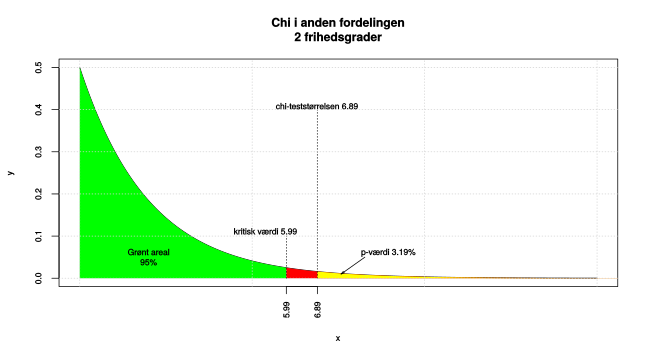
\includegraphics{_main_files/figure-latex/68-1.svg}

I Freestat tastes input i de hvide felter, hvilket resulterer i følgende resultat:

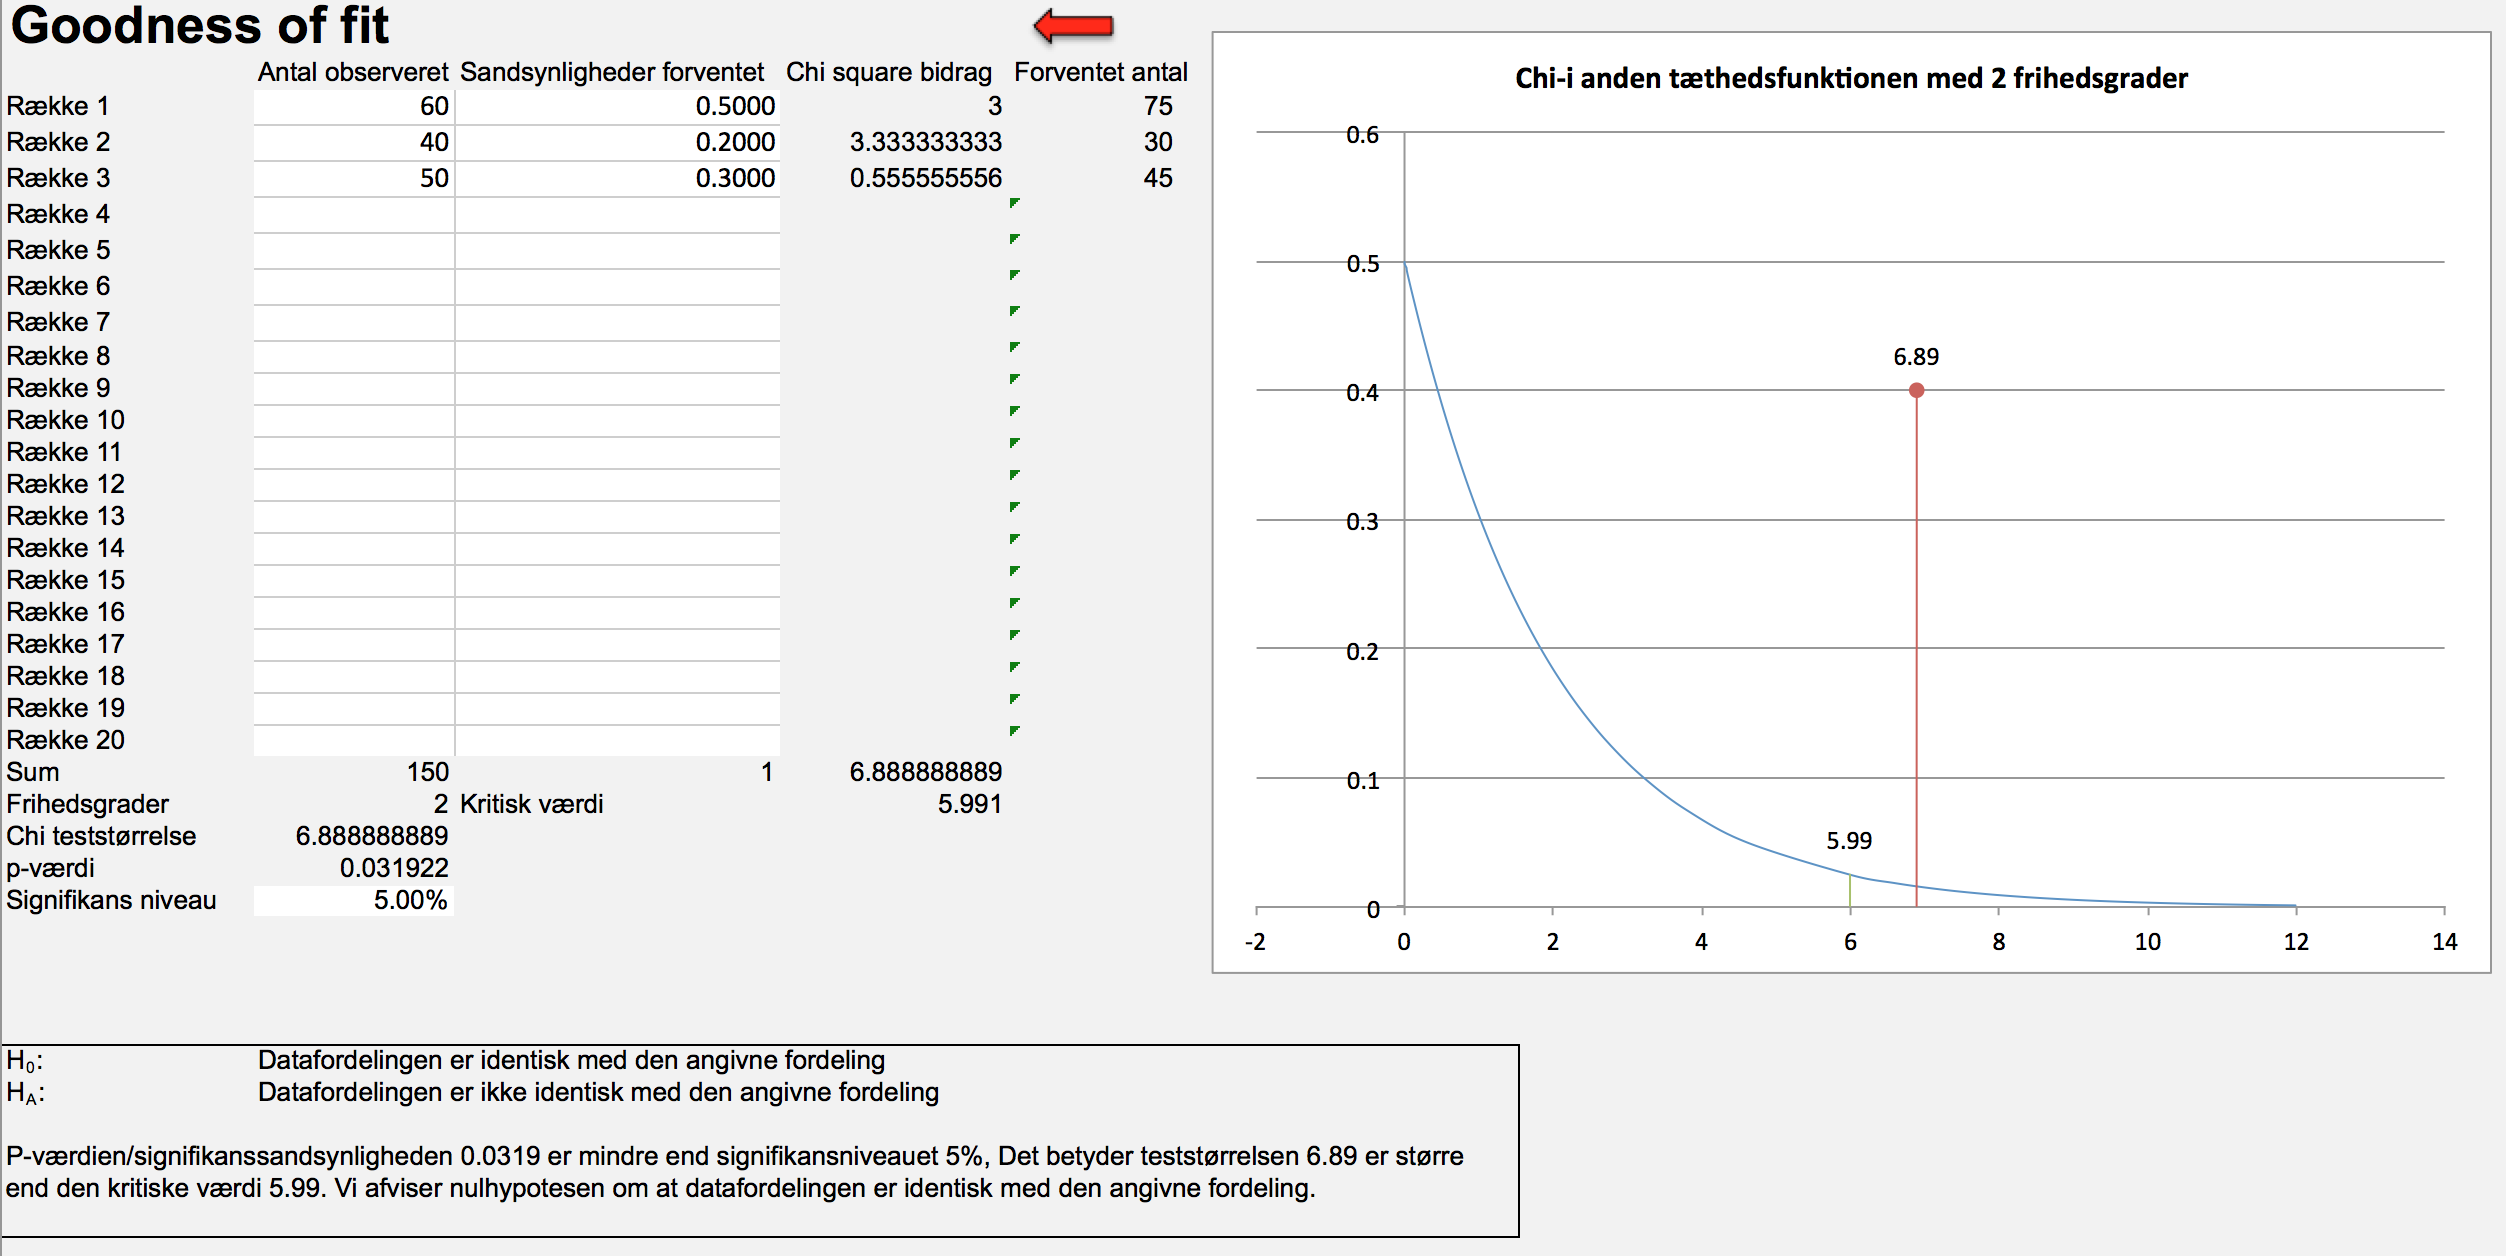
\includegraphics{img/gofbolig.png}

\hypertarget{forudstning}{%
\section{Forudsætning}\label{forudstning}}

En forudsætning for at goodness of fit testet er tilstrækkeligt præcist, er at de forventede værdier E er tilstrækkeligt store. Der er mange forskellige tolkninger, af størrelsen af E cellerne. Nogle nævner celleværdier skal være større end 3 andre 5, det bør under alle omstændigheder nævnes om forudsætningen synes opfyldt. Hvis de forventede værdier er meget små, kan man sammenlægge kategorier, der vil så være et tradeoff med detaljegraden af analysen. Hvis man sammenlægger bør man gøre dette, så det analytisk giver mening.

I eksemplet med boligtyper, havde vi forventede værdier E på hhv. 75, 30 og 45, her var forudsætningen altså opfyldt.

Spørgsmål datasæt karakterer
Undervisningsministeriet har et ønske om at karaktererne på landsplan bør normaliseres omkring 7, hvor der er følgende procentvise vægt på hver karakter

\begin{longtable}[]{@{}ll@{}}
\toprule
Karakter & Ønsket fordeling\tabularnewline
\midrule
\endhead
02 & 10\%\tabularnewline
4 & 25\%\tabularnewline
7 & 30\%\tabularnewline
10 & 25\%\tabularnewline
12 & 10\%\tabularnewline
\bottomrule
\end{longtable}

Der er intet krav til andelen af studerende der består, således drejer fordelingen sig udelukkende om bestået-karakterer.

\href{https://www.dropbox.com/s/mnsmu56cdkl8yyv/Statkarakterer.xlsx?dl=1}{Hent datasættet statkarakterer} for stikprøven for statistikstuderende , betragt kun de beståede studerende, kan populationen antages at følge de generelle retningslinjer?

Svar datasæt karakterer

Vi starter med at se på de beståede 37 studerende, optæl fx. vha. =countif eller =tælhvis i excel for at bestemme antallet af studerende med de respektive karakterer.

\begin{longtable}[]{@{}llll@{}}
\toprule
Karakter & Ønsket fordeling & Observeret antal & Observeret Frekvens\tabularnewline
\midrule
\endhead
02 & 10\% & 9 & 0.2432\tabularnewline
4 & 25\% & 6 & 0.1622\tabularnewline
7 & 30\% & 5 & 0.1351\tabularnewline
10 & 25\% & 12 & 0.3243\tabularnewline
12 & 10\% & 5 & 0.1351\tabularnewline
\bottomrule
\end{longtable}

Vi kan nu bestemme den forventede karakterfordeling hvis karaktererne følger den ønskede fordeling.

\begin{longtable}[]{@{}llll@{}}
\toprule
Karakter & Ønsket fordeling & Forventet antal & Chi i anden bidrag\tabularnewline
\midrule
\endhead
02 & 10\% & 3.7 & 7.5919\tabularnewline
4 & 25\% & 9.25 & 1.1419\tabularnewline
7 & 30\% & 11.1 & 3.3523\tabularnewline
10 & 25\% & 9.25 & 0.8176\tabularnewline
12 & 10\% & 3.7 & 0.4568\tabularnewline
\bottomrule
\end{longtable}

Bemærk forventede værdier er mindre end 5 men større end 3, der kan være problemer med præcisionen. Hvis man ønsker at sammenlægge kategorier giver det ikke mening at lægge 02 og 12 sammen, men gerne 02 og 4 eller 10 og 12. Summen af chi i anden bidrag giver teststørrelsen, dvs:

7.5919+1.1419+3.3523+0.8176=13.3604

Hvilket fører til p-værdien 0.0096 illustreret ved den gule hale herunder, da p-værdien er mindre end 5\% signifikansniveauet forkaster vi nulhypotesen, og konkluderer at statistikkarakterer på Finansøkonom ikke følger den ønskede fordeling. Vi kan ud fra chi i anden bidragene se hvilke karakterer der giver de største afvigelser. Store bidrag betyder store afvigelser mellem det observede og ønskede. Det største bidrag 7.5919 stammer fra 02 karakteren, her er den observerede karakter 9, mens den forventede værdi er 3.7. Der er altså flere studerende, end forventet der får 02. Bemærk for at vi kan udtale os om populationen finansøkonomer, fordres at stikprøven er repræsentativ for finansøkonomer. Stikprøven er ikke udtaget simpelt tilfældigt, da der er tale om 2 bestemte klasser, det kan derfor diskuteres om stikprøven er afspejler populationen korrekt.

\includegraphics{_main_files/figure-latex/gofstatkar-1.svg}

Freestat output bliver:

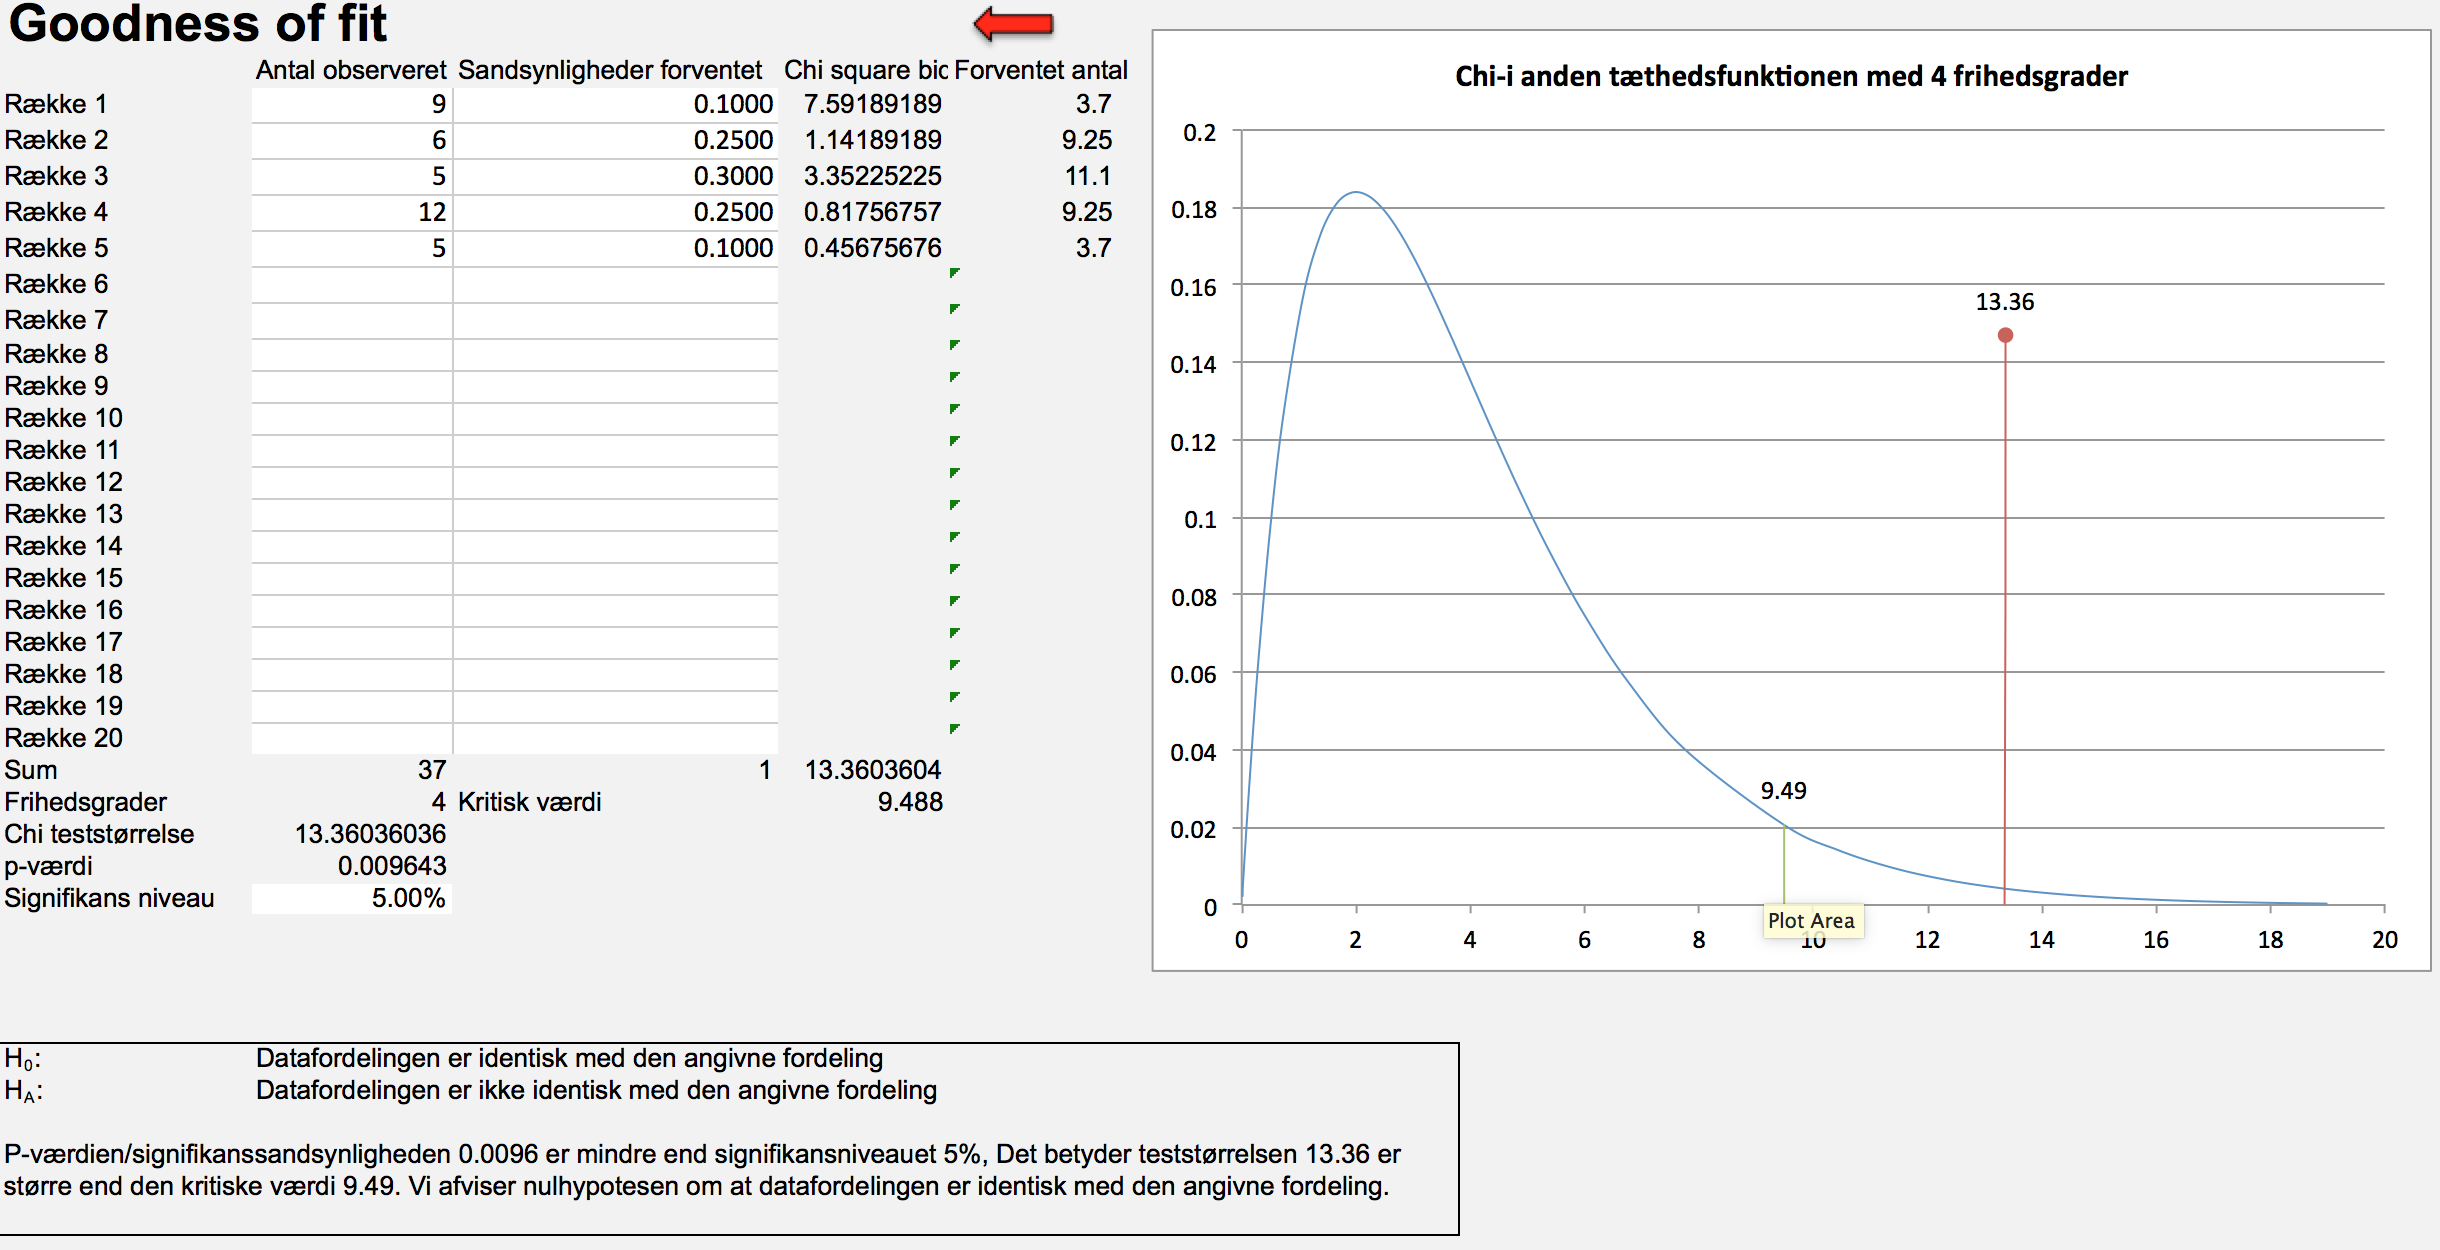
\includegraphics{img/gof.png}

\hypertarget{chi-i-anden-test}{%
\section{Chi i anden test}\label{chi-i-anden-test}}

\#\# Chi i anden test 2

Vi kan analysere kvalitative variable med 2 mulige udfald vha. test af 2 andele. Chi i anden testet er en udvidelse af test af 2 andele. Med chi i anden testen kan man sammenligne kvalitative variable med 2 eller flere mulige udfald. Vi kan benytte chi i anden testet til at undersøge om der er en sammenhæng mellem 2 inddelingskriterier som fx. køn og bestået/ikke bestået, køn og karakter, aldersgruppe og karakter.

Antag et forsikringsselskab har indsamlet data for kunders skadesanmeldelser fordelt på øst og vest for Storebælt. Forsikringsselskabet ønsker at undersøge om der er forskel i andelen af kunder der anmelder skader i Øst- og Vestdanmark. Følgende data er angivet

\begin{longtable}[]{@{}llll@{}}
\toprule
\textbf{\emph{Observeret}} & Ingen skader anmeldt & 1 eller flere skader & Total\tabularnewline
\midrule
\endhead
Østdanmark & 300 & 300 & 600\tabularnewline
Vestdanmark & 250 & 150 & 400\tabularnewline
Total & 550 & 450 & 1000\tabularnewline
\bottomrule
\end{longtable}

Vi kan teste om der er forskel på om der er forskel på andelen af anmeldte skader i Øst- og Vestdanmark vha. chi i anden testet. Vi har følgende hypoteser.

\[H_0: Der\ er\ uafhæ\ \ ngighed\ mellem\ ræ\ kke-\ og\ sø\ jlekriterierne\]\[H_1: Der\ er\ afhæ\ \ ngighed\ mellem\ ræ\ kke-\ og\ sø\ jlekriterierne\]

Eller mere præcist i dette tilfælde:

\[H_0: Der\ er\ uafhæ\ \ ngighed\ mellem\ landsdel\ og\ skadesanmeldelse\]\[H_1: Der\ er\ afhæ\ \ ngighed\ mellem\ landsdel\ og\ skadesanmeldelse\]

Hvis nulhypotesen forkastes påvirker landsdelen kunder kommer fra altså andelen af anmeldte skader.

\hypertarget{uafhngighed}{%
\subsection{Uafhængighed}\label{uafhngighed}}

Definitionen af uafhængighed mellem 2 hændelser A og B er at sandsynligheden for fælleshændelsen er lig med produktet af sandsynlighederne for enkelthændelserne som formel skriver vi:
\[P(A\cap B)=P(A)\cdot P(B)\]

Vores hændelse A kan fx. være kunden stammer fra Østdanmark, og hændelse B at kunden har ikke anmeldt skader. Vi får da følgende ligning:
\[P(Ø\ \ stdanmark\cap 0\ skader)=P(Ø\ \ stdanmark)\cdot P(0\ skader)\]
Vi kan omskrive dette til:
\[P(Ø\ \ stdanmark\cap0\ skader)=P(Ø\ \ stdanmark)\cdot P(0\ skader)\Leftrightarrow \frac{300}{1000}=\frac{600}{1000}\cdot \frac{550}{1000} \Leftrightarrow \]\[1000\cdot\frac{300}{1000}=1000\cdot \frac{600\cdot550}{1000\cdot1000} \Leftrightarrow 300= \frac{600\cdot550}{1000}\]
Her er venstresiden i ligningen jo den observerede celleværdi. Hvis der er uafhængighed under nulhypotesen, vil vi forvente at den observerede værdi, er lig med venstresiden, som vi kalder den forventede værdi. Hvis der er perfekt uafhængighed mellem landsdel og skadesanmeldelse, ville vi altså i hver celle forvente værdien:
\[\frac{ræ\ \ kkesum\cdot sø\ jlesum}{totalsum}\]

Vi får derfor følgende matrice.

\begin{longtable}[]{@{}llll@{}}
\toprule
\begin{minipage}[b]{0.09\columnwidth}\raggedright
\textbf{\emph{Forventet}}\strut
\end{minipage} & \begin{minipage}[b]{0.23\columnwidth}\raggedright
Ingen skader anmeldt\strut
\end{minipage} & \begin{minipage}[b]{0.28\columnwidth}\raggedright
1 eller flere skader\strut
\end{minipage} & \begin{minipage}[b]{0.28\columnwidth}\raggedright
Total\strut
\end{minipage}\tabularnewline
\midrule
\endhead
\begin{minipage}[t]{0.09\columnwidth}\raggedright
Østdanmark\strut
\end{minipage} & \begin{minipage}[t]{0.23\columnwidth}\raggedright
\(\frac{ræ\ \ kkesum\cdot sø\ jlesum}{totalsum}=\frac{600\cdot 550}{1000}=330\)\strut
\end{minipage} & \begin{minipage}[t]{0.28\columnwidth}\raggedright
\(\frac{ræ\ \ kkesum\cdot sø\ jlesum}{totalsum}=\frac{600\cdot 450}{1000}=270\)\strut
\end{minipage} & \begin{minipage}[t]{0.28\columnwidth}\raggedright
600\strut
\end{minipage}\tabularnewline
\begin{minipage}[t]{0.09\columnwidth}\raggedright
Vestdanmark\strut
\end{minipage} & \begin{minipage}[t]{0.23\columnwidth}\raggedright
\(\frac{ræ\ \ kkesum\cdot sø\ jlesum}{totalsum}=\frac{400\cdot 550}{1000}=220\)\strut
\end{minipage} & \begin{minipage}[t]{0.28\columnwidth}\raggedright
\(\frac{ræ\ \ kkesum\cdot sø\ jlesum}{totalsum}=\frac{400\cdot 450}{1000}=180\)\strut
\end{minipage} & \begin{minipage}[t]{0.28\columnwidth}\raggedright
400\strut
\end{minipage}\tabularnewline
\begin{minipage}[t]{0.09\columnwidth}\raggedright
Total\strut
\end{minipage} & \begin{minipage}[t]{0.23\columnwidth}\raggedright
550\strut
\end{minipage} & \begin{minipage}[t]{0.28\columnwidth}\raggedright
450\strut
\end{minipage} & \begin{minipage}[t]{0.28\columnwidth}\raggedright
1000\strut
\end{minipage}\tabularnewline
\bottomrule
\end{longtable}

Vi kan nu beregne chi i anden cellebidragene med samme formel som for goodness of fit testet:

\[\frac{(O-E)^2}{E}\]

\begin{longtable}[]{@{}llll@{}}
\toprule
\begin{minipage}[b]{0.09\columnwidth}\raggedright
\textbf{\emph{Chi celle bidrag}}\strut
\end{minipage} & \begin{minipage}[b]{0.23\columnwidth}\raggedright
Ingen skader anmeldt\strut
\end{minipage} & \begin{minipage}[b]{0.28\columnwidth}\raggedright
1 eller flere skader\strut
\end{minipage} & \begin{minipage}[b]{0.28\columnwidth}\raggedright
Total\strut
\end{minipage}\tabularnewline
\midrule
\endhead
\begin{minipage}[t]{0.09\columnwidth}\raggedright
Østdanmark\strut
\end{minipage} & \begin{minipage}[t]{0.23\columnwidth}\raggedright
\(\frac{(300-330)^2}{330}=2.7272727\)\strut
\end{minipage} & \begin{minipage}[t]{0.28\columnwidth}\raggedright
\(\frac{(300-270)^2}{270}=3.3333333\)\strut
\end{minipage} & \begin{minipage}[t]{0.28\columnwidth}\raggedright
\strut
\end{minipage}\tabularnewline
\begin{minipage}[t]{0.09\columnwidth}\raggedright
Vestdanmark\strut
\end{minipage} & \begin{minipage}[t]{0.23\columnwidth}\raggedright
\(\frac{(250-220)^2}{220}=4.0909091\)\strut
\end{minipage} & \begin{minipage}[t]{0.28\columnwidth}\raggedright
\(\frac{(150-180)^2}{180}=5\)\strut
\end{minipage} & \begin{minipage}[t]{0.28\columnwidth}\raggedright
\strut
\end{minipage}\tabularnewline
\begin{minipage}[t]{0.09\columnwidth}\raggedright
Total\strut
\end{minipage} & \begin{minipage}[t]{0.23\columnwidth}\raggedright
\strut
\end{minipage} & \begin{minipage}[t]{0.28\columnwidth}\raggedright
\strut
\end{minipage} & \begin{minipage}[t]{0.28\columnwidth}\raggedright
15.15\strut
\end{minipage}\tabularnewline
\bottomrule
\end{longtable}

Teststørrelsen bliver 15.15, denne bruger vi til at beregne p-værdien for testet af uafhængighed. Antallet af frihedsgrader for chi i anden fordelingen er antallet af rækkeinddelingskriterier Østdanmark og Vestdanmark minus 1, gange antallet af søjleinddelingskriterier 0 skader og flere end 0 skader minus 1, dvs. \[(r-1)\cdot(s-1)=(2-1)\cdot(2-1)=1\cdot1=1\]
Vi får p-værdien 0.000099, hvilket er klart mindre end signifikansniveauet på 5\%, arealet er så lille vi ikke kan se det på figuren nedenfor. Vi forkaster altså nulhypotesen og konstaterer der er afhængighed mellem landsdel og anmeldte skader. Landsdelen som kunden stammer fra, påvirker altså antallet af anmeldte skader. Vi kan nu se om der er chi i anden bidrag, der er meget store og dermed bidrager stæ til konklusionen om afhængighed. Der er ikke en voldsom forskel i størrelserne på chi i anden bidragene, men når vi ser på observeret mod forventet, ser vi at 150 anmelder skader, det var forventet at 180 personer fra Vestdanmark anmelder skader. Denne tendens er modsat for Østdanmark. Vestdanmark anmelder altså færre skader end Østdanmark.

Ligesom for goodness of fit testet, skal de forventede værdier have en vis størrelse for at vore konklusioner er præcise. Forudsætningen om forventede værdier større end 5 er opfyldt for alle celler.

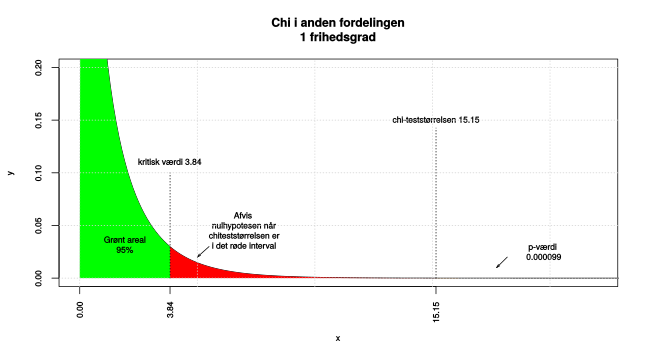
\includegraphics{_main_files/figure-latex/chi45-1.svg}

Freestat output bliver
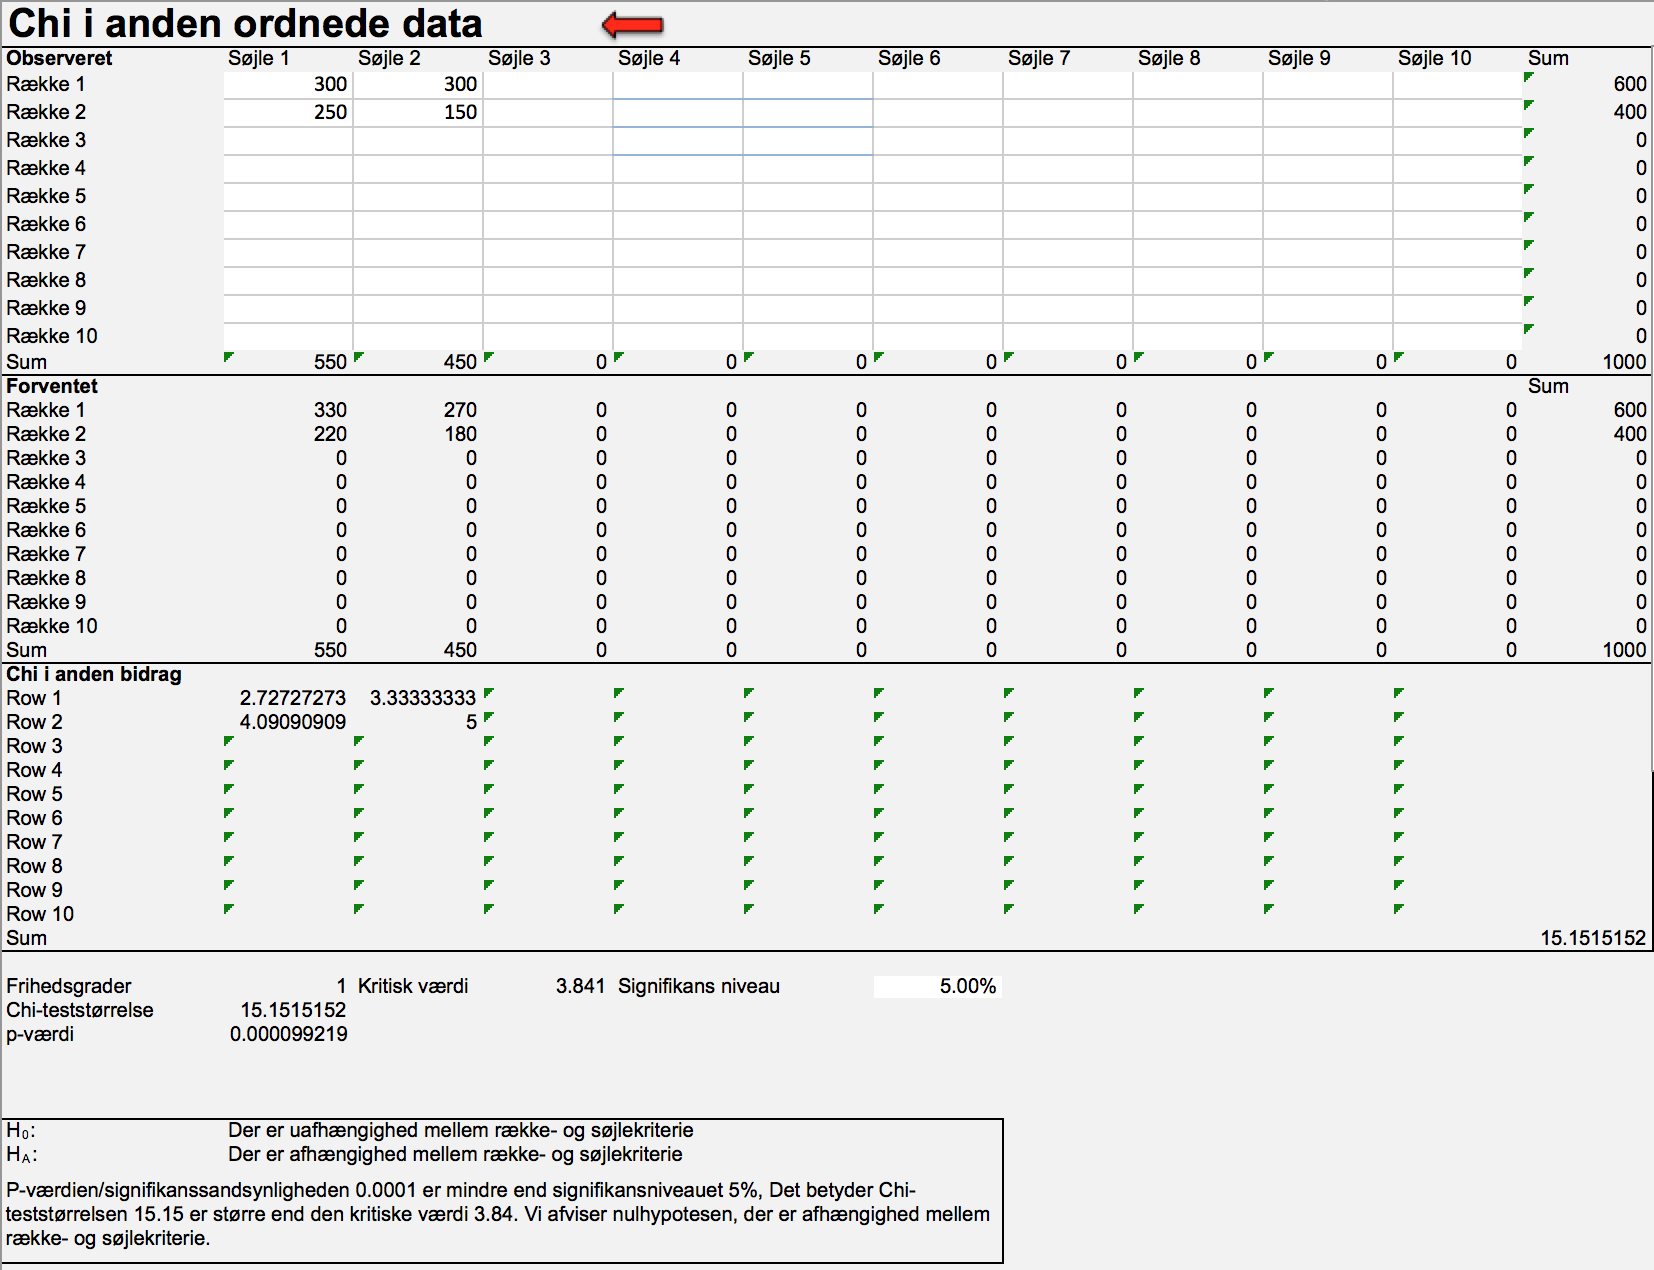
\includegraphics{img/chiskade.png}

\hypertarget{anmeldte-skader-fordelt-pa-regioner-og-antal-skader}{%
\subsection{Anmeldte skader fordelt på regioner og antal skader}\label{anmeldte-skader-fordelt-pa-regioner-og-antal-skader}}

Vi antager nu der foreligger mere specifikke data for undersøgelsen omkring geografisk placering og skadesanmeldelse.Vi har finere inddeling på region og antal skader.

\begin{longtable}[]{@{}lllll@{}}
\toprule
\textbf{\emph{Observeret}} & 0 skader & 1 skade & 2 eller flere skader & Total\tabularnewline
\midrule
\endhead
Hovedstaden & 150 & 125 & 50 & 325\tabularnewline
Sjælland & 150 & 100 & 25 & 275\tabularnewline
Syddanmark & 75 & 30 & 10 & 115\tabularnewline
Midtjylland & 75 & 40 & 10 & 125\tabularnewline
Nordjylland & 100 & 45 & 15 & 160\tabularnewline
Total & 550 & 340 & 110 & 1000\tabularnewline
\bottomrule
\end{longtable}

Vi kan teste om der er forskel på om der er forskel på andelen af anmeldte skader i Øst- og Vestdanmark vha. chi i anden testet. Vi har følgende hypoteser.

\[H_0: Der\ er\ uafhæ\ \ ngighed\ mellem\ region\ og\ antal skader\]\[H_1: Der\ er\ afhæ\ \ ngighed\ mellem\ region\ og\ antal skader\]

Hvis nulhypotesen forkastes påvirker regionen kunder kommer fra altså antallet af anmeldte skader.

Vi beregner de forventede værdier efter den sædvanlige formel:

\[\frac{ræ\ \ kkesum\cdot sø\ jlesum}{totalsum}\]

Hvilket giver følgende matrix

\begin{longtable}[]{@{}lllll@{}}
\toprule
\textbf{\emph{Forventet}} & 0 skader & 1 skade & 2 eller flere skader & Total\tabularnewline
\midrule
\endhead
Hovedstaden & 178.75 & 110.5 & 35.75 & 325\tabularnewline
Sjælland & 151.25 & 93.5 & 30.25 & 275\tabularnewline
Syddanmark & 63.25 & 39.1 & 12.65 & 115\tabularnewline
Midtjylland & 68.75 & 42.5 & 13.75 & 125\tabularnewline
Nordjylland & 88 & 54.4 & 17.6 & 160\tabularnewline
Total & 550 & 340 & 110 & 1000\tabularnewline
\bottomrule
\end{longtable}

Vi kan nu beregne chi i anden cellebidragene med samme formel som for goodness of fit testet:

\[\frac{(O-E)^2}{E}\]

\begin{longtable}[]{@{}lllll@{}}
\toprule
\textbf{\emph{Chi celle bidrag}} & 0 skader & 1 skade & 2 eller flere skader & Total\tabularnewline
\midrule
\endhead
Hovedstaden & 4.6241259 & 1.9027149 & 5.6800699 & 12.2069107\tabularnewline
Sjælland & 0.0103306 & 0.4518717 & 0.911157 & 1.3733593\tabularnewline
Syddanmark & 2.1828063 & 2.1179028 & 0.5551383 & 4.8558475\tabularnewline
Midtjylland & 0.5681818 & 0.1470588 & 1.0227273 & 1.7379679\tabularnewline
Nordjylland & 1.6363636 & 1.6242647 & 0.3840909 & 3.6447193\tabularnewline
Total & 9.0218082 & 6.2438129 & 8.5531835 & 23.8188046\tabularnewline
\bottomrule
\end{longtable}

Teststørrelsen bliver 23.82, denne bruger vi til at beregne p-værdien for testet af uafhængighed. Antallet af frihedsgrader bliver
\[(r-1)\cdot(s-1)=(5-1)\cdot(3-1)=4\cdot 2=8\]
Vi får p-værdien 0.002458, hvilket er klart mindre end signifikansniveauet på 5\%. Vi forkaster nulhypotesen og konstaterer, der er afhængighed mellem region og antal anmeldte skader. Regionen som kunden stammer fra, påvirker altså antallet af anmeldte skader. Vi kan se, der er chi i anden bidrag, der er store for region København, disse bidrager kraftigt til konklusionen om afhængighed. Københavnerne anmelder flere skader end forventet, dermed er der færre københavnere end forventet, der ikke anmelder skader.

Forudsætningen om forventede værdier større end 5 er opfyldt for alle celler.

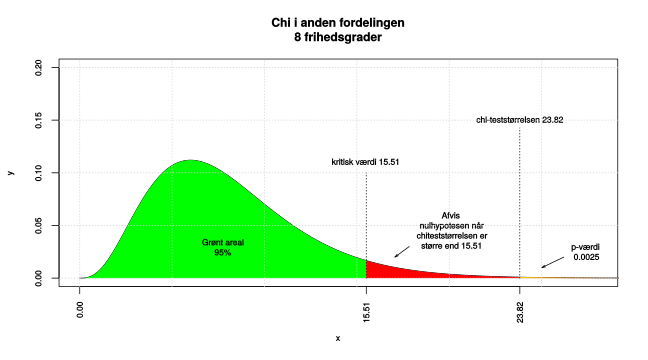
\includegraphics{_main_files/figure-latex/chi46-1.svg}

Freestat output bliver
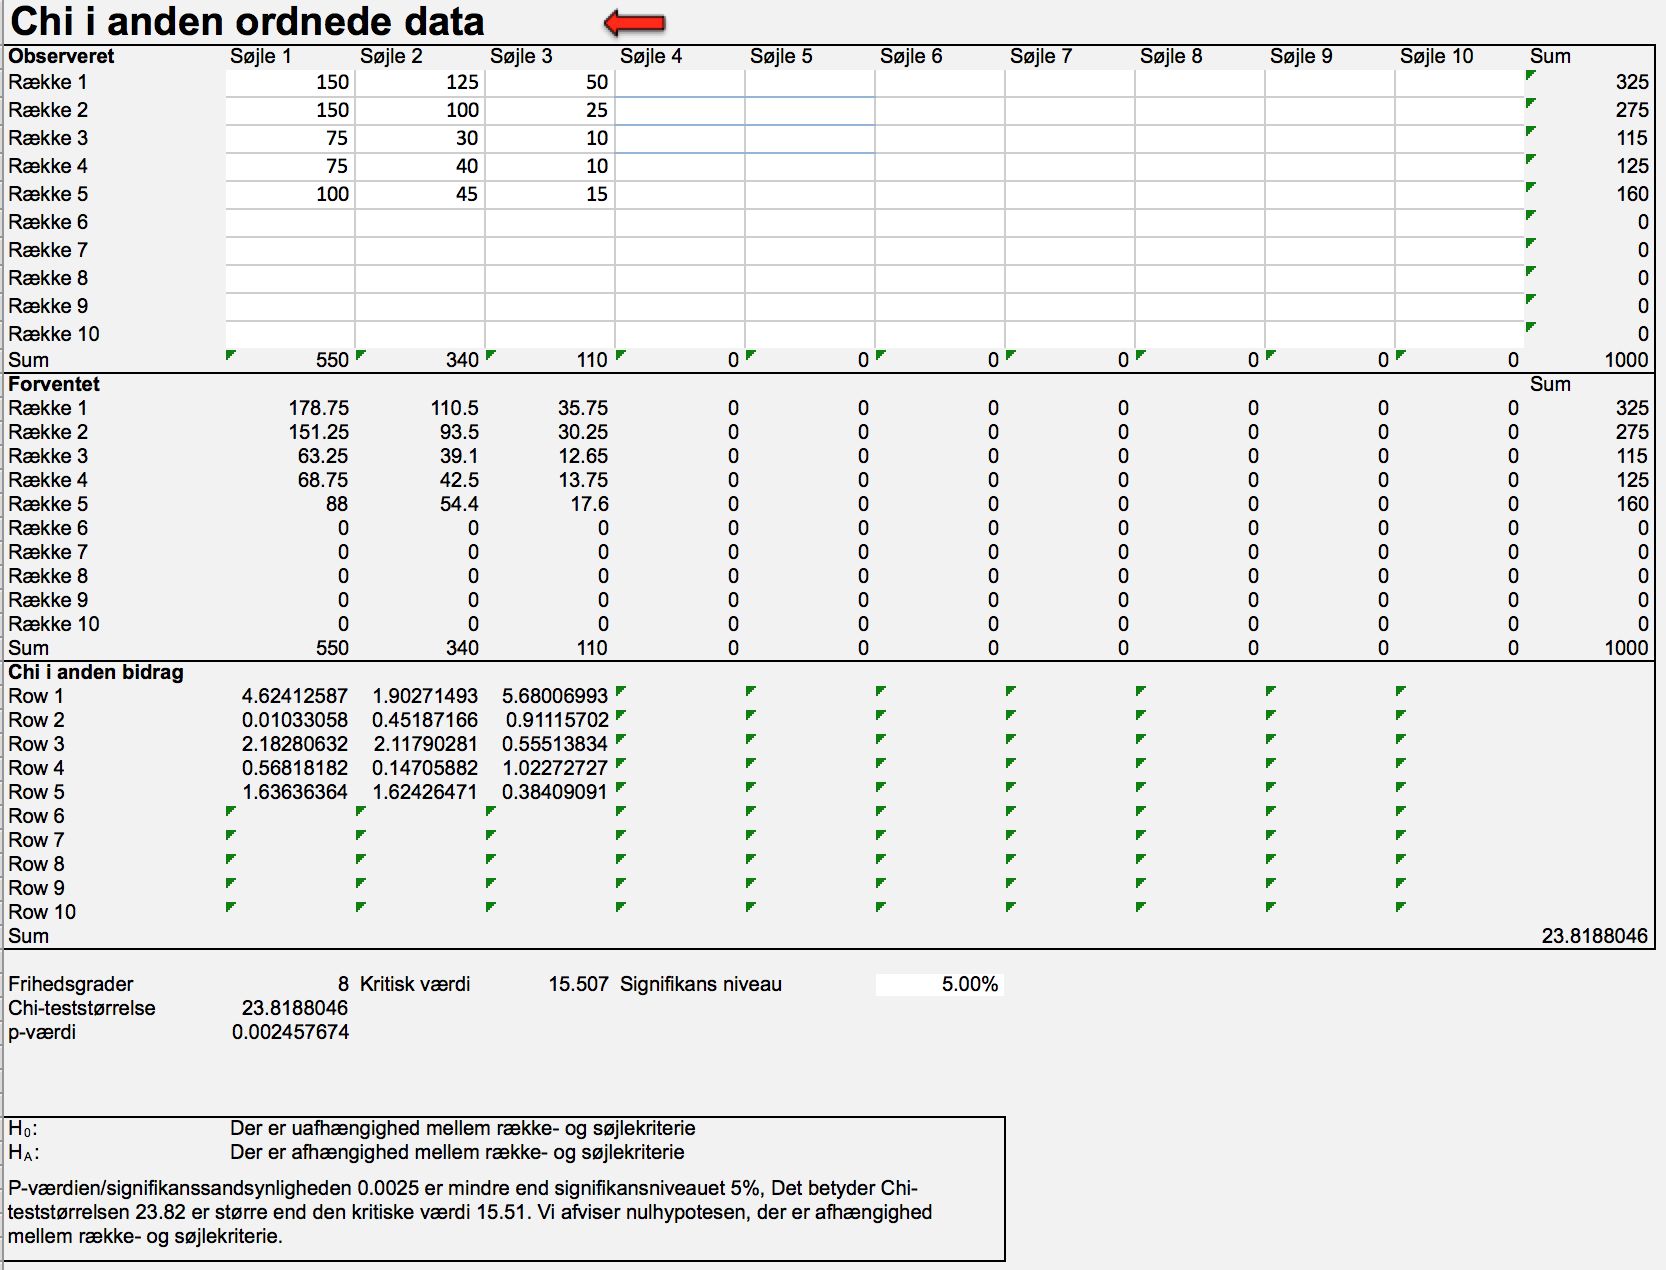
\includegraphics{img/chiskade2.png}

Spørgsmål Titanic

I 1912 forliste Titanic, vi har i filen oplysninger om passagererne. Har man har større chance for at overleve, hvis man er velhavende? Vi har ikke oplysninger om passagerernes formuer, men vi kan bruge oplysningerne om billetterne som en proxy for velstand. Variablen pclass angiver hvilken billet den pågældende passager havde, 1. klasse er dyrest. Variablen survived fortæller om en passager overlevede 1 eller døde 0. Data er i filen \href{https://drive.google.com/uc?export=download\&id=0B1E7VnhxsDMlYWJOOG5yamNoOTQ}{Titanic}.

Svar Titanic

Vi sorterer passagerer efter billet og om de har overlevet.

\begin{longtable}[]{@{}llll@{}}
\toprule
\textbf{\emph{Observeret}} & Døde & Overlevede & Total\tabularnewline
\midrule
\endhead
1. Klasse & 123 & 200 & 323\tabularnewline
2. Klasse & 158 & 119 & 277\tabularnewline
3. Klasse & 528 & 181 & 709\tabularnewline
Total & 809 & 500 & 1309\tabularnewline
\bottomrule
\end{longtable}

Vi kan teste om der er billettype betyder noget for overlevelse. Vi får følgende hypoteser:

\[H_0: Der\ er\ uafhæ\ \ ngighed\ mellem\ passagerklasse\ og\ overlevelse\]\[H_1: Der\ er\ afhæ\ \ ngighed\ mellem\ passagerklasse\ og\ overlevelse\]

Hvis nulhypotesen forkastes betyder passagerklasse noget for noget for overlevelsen

Vi beregner de forventede værdier:

\[\frac{ræ\ \ kkesum\cdot sø\ jlesum}{totalsum}\]

Hvilket giver følgende matrix

\begin{longtable}[]{@{}llll@{}}
\toprule
\textbf{\emph{Forventet}} & Døde & Overlevede & Total\tabularnewline
\midrule
\endhead
1. Klasse & 199.62 & 123.38 & 323\tabularnewline
2. Klasse & 171.19 & 105.81 & 277\tabularnewline
3. Klasse & 438.18 & 270.82 & 709\tabularnewline
Total & 809 & 500 & 1309\tabularnewline
\bottomrule
\end{longtable}

Vi kan nu beregne chi i anden cellebidragene med samme formel som for goodness of fit testet:

\[\frac{(O-E)^2}{E}\]

\begin{longtable}[]{@{}llll@{}}
\toprule
\textbf{\emph{Chi celle bidrag}} & Døde & Overlevede & Total\tabularnewline
\midrule
\endhead
1. Klasse & 29.4111 & 47.5871 & 76.9982\tabularnewline
2. Klasse & 1.0169 & 1.6453 & 2.6622\tabularnewline
3. Klasse & 18.4105 & 29.7882 & 48.1987\tabularnewline
Total & 48.8385 & 79.0207 & 127.8592\tabularnewline
\bottomrule
\end{longtable}

Teststørrelsen bliver 127.86, denne bruger vi til at beregne p-værdien for testet af uafhængighed. Antallet af frihedsgrader bliver
\[(r-1)\cdot(s-1)=(3-1)\cdot(2-1)=2\cdot 1=2\]
Vi får p-værdien 0, hvilket er klart mindre end signifikansniveauet på 5\%. Vi forkaster nulhypotesen og konstaterer, der er afhængighed mellem passagerklasse og overlevelse.

Forudsætningen om forventede værdier større end 5 er opfyldt for alle celler.

Vi kan se at 200 1. klasses passagerer overlevede mod forventet 123.38 under nulhypotesen, hvilket giver et meget stort chi i anden bidrag. Omvendt overlevede kun 181 3. klasses passagerer mod 270.82 forventet under nulhypotesen. Der var altså væstentlig større chance for overlevelse hvis man er velhavende.

Spørgsmål bankansatte

Vi ser på data for bankansatte i filen \href{https://drive.google.com/uc?export=download\&id=0B1E7VnhxsDMlRENKWWxlNlBXbmM}{Bankdata filen}. Er der sammenhæng mellem jobfunktion og køn?

Svar bankansatte

Vi sorterer personalet efter jobfunktion og køn.

\begin{longtable}[]{@{}llll@{}}
\toprule
\textbf{\emph{Observeret}} & Kvinde & Mand & Total\tabularnewline
\midrule
\endhead
Administration & 206 & 157 & 363\tabularnewline
Sikkerhedspersonale & 0 & 27 & 27\tabularnewline
Ledelse & 10 & 74 & 84\tabularnewline
Total & 216 & 258 & 474\tabularnewline
\bottomrule
\end{longtable}

Vi kan teste om der er billettype betyder noget for overlevelse. Vi får følgende hypoteser:

\[H_0: Der\ er\ uafhæ\ \ ngighed\ mellem\ jobfunktion\ og\ kø\ n\]\[H_1: Der\ er\ afhæ\ \ ngighed\ mellem\ jobfunktion\ og\ kø\ n\]

Hvis nulhypotesen forkastes har køn betydning for jobfunktion.

Vi beregner de forventede værdier:

\[\frac{ræ\ \ kkesum\cdot sø\ jlesum}{totalsum}\]

Hvilket giver følgende matrix

\begin{longtable}[]{@{}llll@{}}
\toprule
\textbf{\emph{Forventet}} & Kvinde & Mand & Total\tabularnewline
\midrule
\endhead
Administration & 165.42 & 197.58 & 363\tabularnewline
Sikkerhedspersonale & 12.3 & 14.7 & 27\tabularnewline
Ledelse & 38.28 & 45.72 & 84\tabularnewline
Total & 216 & 258 & 474\tabularnewline
\bottomrule
\end{longtable}

Vi kan nu beregne chi i anden cellebidragene med samme formel som for goodness of fit testet:

\[\frac{(O-E)^2}{E}\]

\begin{longtable}[]{@{}llll@{}}
\toprule
\textbf{\emph{Chi celle bidrag}} & Kvinde & Mand & Total\tabularnewline
\midrule
\endhead
Administration & 9.9561 & 8.3354 & 18.2915\tabularnewline
Sikkerhedspersonale & 12.3038 & 10.3009 & 22.6047\tabularnewline
Ledelse & 20.8909 & 17.4901 & 38.381\tabularnewline
Total & 43.1508 & 36.1264 & 79.2772\tabularnewline
\bottomrule
\end{longtable}

Teststørrelsen bliver 79.28, denne bruger vi til at beregne p-værdien for testet af uafhængighed. Antallet af frihedsgrader bliver
\[(r-1)\cdot(s-1)=(3-1)\cdot(2-1)=2\cdot 1=2\]
Vi får en meeget lille p-værdi afrundet til 0, hvilket er klart mindre end signifikansniveauet på 5\%. Vi forkaster nulhypotesen og konstaterer, der er afhængighed mellem jobfunktion og køn.

Forudsætningen om forventede værdier større end 5 er opfyldt for alle celler.

Udfra tabellerne ses at mænd er underrepræsenteret i administrationen og overrepræsenteret i sikkerhedspersonale og ledelse.

Spørgsmål bankansatte

Vi ser fortsat på data for bankansatte i filen \href{https://drive.google.com/uc?export=download\&id=0B1E7VnhxsDMlRENKWWxlNlBXbmM}{Bankdata filen}. Er der sammenhæng mellem jobfunktion og minoritet? Minoritet er ikke-hvide.

Svar bankansatte
Vi sorterer personalet efter jobfunktion og køn.

\begin{longtable}[]{@{}llll@{}}
\toprule
\textbf{\emph{Observeret}} & Ikke-minoritet & minoritet & Total\tabularnewline
\midrule
\endhead
Administration & 276 & 87 & 363\tabularnewline
Sikkerhedspersonale & 14 & 13 & 27\tabularnewline
Ledelse & 80 & 4 & 84\tabularnewline
Total & 370 & 104 & 474\tabularnewline
\bottomrule
\end{longtable}

Vi kan teste om minoritet betyder noget for jobfunktion. Vi får følgende hypoteser:

\[H_0: Der\ er\ uafhæ\ \ ngighed\ mellem\ jobfunktion\ og\ minoritet\]\[H_1: Der\ er\ afhæ\ \ ngighed\ mellem\ jobfunktion\ og\ minoritet\]

Hvis nulhypotesen forkastes betyder det at tilhører man en minoritet har dette betydning for jobfunktionen.

Vi beregner de forventede værdier:

\[\frac{ræ\ \ kkesum\cdot sø\ jlesum}{totalsum}\]

Hvilket giver følgende matrix

\begin{longtable}[]{@{}llll@{}}
\toprule
\textbf{\emph{Forventet}} & Ikke-minoritet & Minoritet & Total\tabularnewline
\midrule
\endhead
Administration & 283.35 & 79.65 & 363\tabularnewline
Sikkerhedspersonale & 21.08 & 5.92 & 27\tabularnewline
Ledelse & 65.57 & 18.43 & 84\tabularnewline
Total & 370 & 104 & 474\tabularnewline
\bottomrule
\end{longtable}

Vi kan nu beregne chi i anden cellebidragene med samme formel som for goodness of fit testet:

\[\frac{(O-E)^2}{E}\]

\begin{longtable}[]{@{}llll@{}}
\toprule
\textbf{\emph{Chi celle bidrag}} & Ikke-minoritet & minoritet & Total\tabularnewline
\midrule
\endhead
Administration & 0.1909 & 0.6791 & 0.87\tabularnewline
Sikkerhedspersonale & 2.3756 & 8.4518 & 10.8274\tabularnewline
Ledelse & 3.1758 & 11.2985 & 14.4743\tabularnewline
Total & 5.7423 & 20.4294 & 26.1717\tabularnewline
\bottomrule
\end{longtable}

Teststørrelsen bliver 26.17, denne bruger vi til at beregne p-værdien for testet af uafhængighed. Antallet af frihedsgrader bliver
\[(r-1)\cdot(s-1)=(3-1)\cdot(2-1)=2\cdot 1=2\]
Vi får en lille p-værdi på 0.000002, hvilket er klart mindre end signifikansniveauet på 5\%. Vi forkaster nulhypotesen og konstaterer, der er afhængighed mellem jobfunktion og om man tilhører en minoritet.

Forudsætningen om forventede værdier større end 5 er opfyldt for alle celler.

Udfra tabellerne ses at minoriteter er overrepræsenteret blandt administration og sikkerhedspersonale og underrepræsenteret i ledelsen.

\hypertarget{selvtest}{%
\section{Selvtest}\label{selvtest}}

Selvtest Chi i anden investeringsfonde med videoløsninger

\hypertarget{selvtest-1}{%
\section{Selvtest}\label{selvtest-1}}

Selvtest Chi i anden realkredit med videoløsninger

\hypertarget{anova}{%
\chapter{ANOVA}\label{anova}}

\hypertarget{Sentry_noJS}{}
Sentry Page Protection

\hypertarget{Sentry_redirecting}{}
Please Wait\ldots{}

ANOVA er en metode til at sammenligne middelværdierne for mere end to kvantitative variable. Skal man sammenligne to middelværdier med varianshomogenitet, benytter man pooled t-test, er der mere end 2 middelværdier benyttes ANOVA F-test . Forudsætningerne for at benytte testen er at populationerne er normalfordelte og har samme varians.

ANOVA er en forkortelse af analysis of variances, man tester om middelværdierne er ens vha. varianserne.
Vi undersøger om k populationer har samme middelværdi, hypoteserne bliver:

\[H_0:\mu_1=\mu_2=...=\mu_k\]\[H_1:Ikke\ alle\ middelvæ\ rdier\ er\ ens.\]

Den totale variation SST kan opdeles i SSW og SSA hvor, SSW er variationen indenfor de k grupper, SSA er variationen mellem grupperne.

Hvis variationen indenfor grupperne SSW er lille i forhold til variationen mellem grupperne SSA, er middelværdierne ikke ens.

Herunder er et eksempel, hvor populationerne er dagsafkast for aktier, variationen indenfor grupperne SSW er lille i forhold til variationen mellem grupperne SSA, derfor er middelværdierne signifikant forskellige.

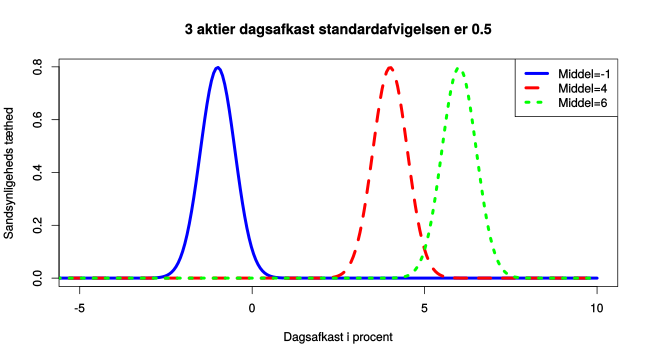
\includegraphics{_main_files/figure-latex/anova1-1.svg}

Herunder er en figur med dagsafkast for aktier, hvor variationen indenfor grupperne SSW er stor i forhold til variationen mellem grupperne SSA, derfor er middelværdierne ikke signifikant forskellige.

\includegraphics{_main_files/figure-latex/anova2-1.svg}

Herunder er et eksempel hvor forudsætningen om varianshomogenitet ikke er opfyldt, de 3 aktier har forskelligt variation.

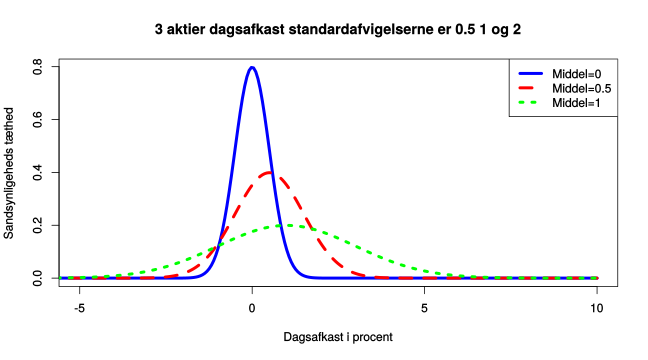
\includegraphics{_main_files/figure-latex/anova3-1.svg}

Et forsikringsselskab har udviklet 4 forskellige layouts til information om skadesdækning. Brugerne udsættes vilkårligt for et af de 4 layouts, selskabet registrerer tiderne for besøgene på hjemmesiderne for at afgøre hvilket design, der er optimalt mht. brugervenlighed og overskuelighed.

Hent datasættet Hjemmesidedesigns besøgstider i millisekunder, der viser de 359 observede besøgstider på de 4 hjemmesider.

Forsikringsselskabet ønsker at undersøge om der er forskel på besøgstiderne, vi opstiller hypoteserne:

\[H_0:\mu_{Design 1}=\mu_{Design 2}=\mu_{Design 3}=\mu_{Design 4}\]\[H_1:Ikke\ alle\ middelvæ\ rdier\ er\ ens\ for\ de\ 4\ designs.\]

Freestat output
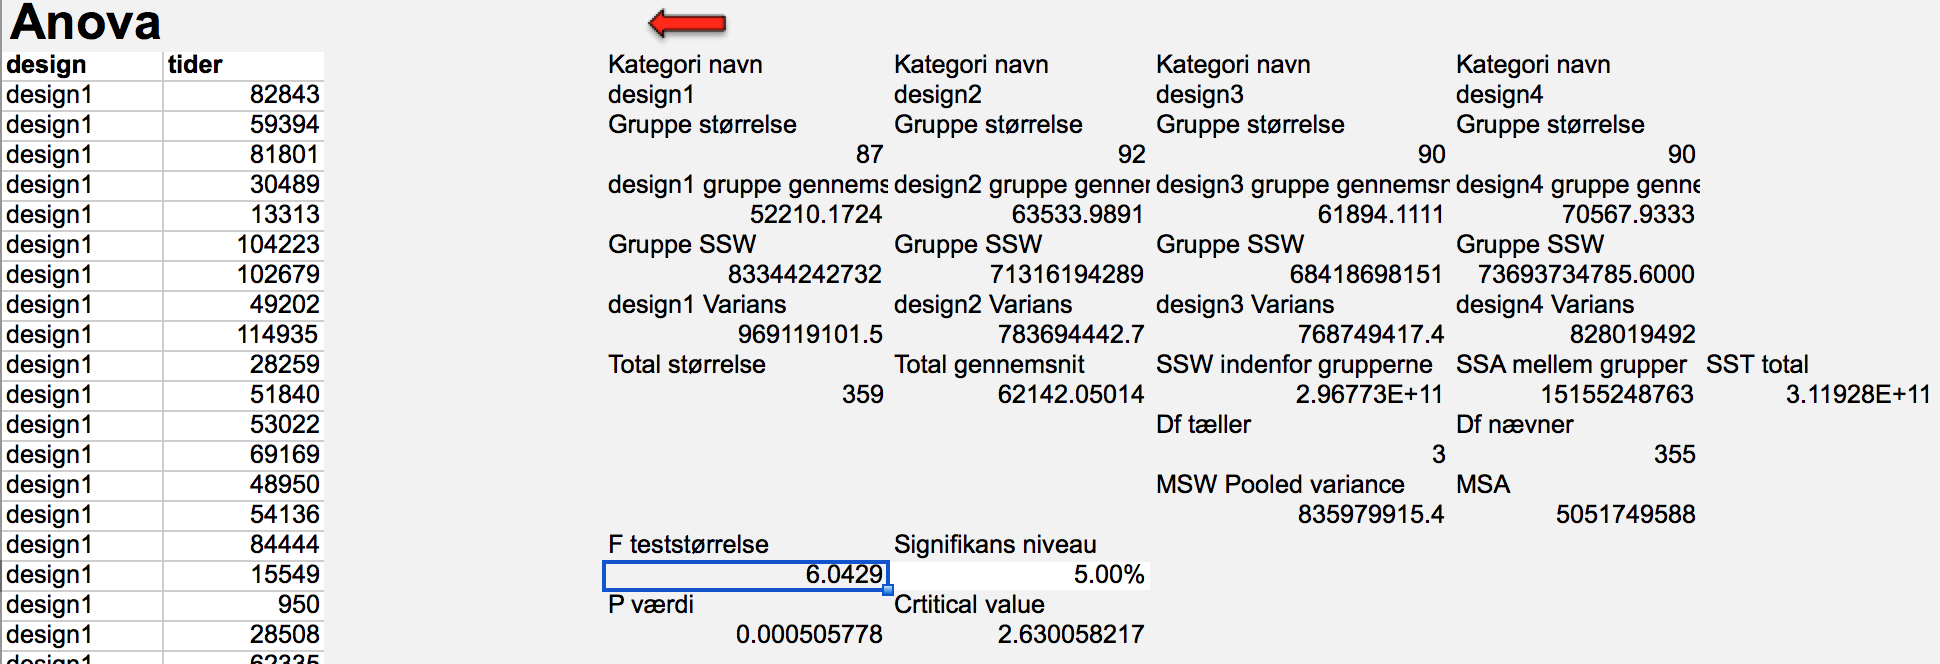
\includegraphics{img/anova1.png}

Vi får en F-teststørrelse på 6.0429, der resulterer i en p-værdi på 0.0005, hvilket er under signifikansniveauet på 0.05. Vi kan forkaster altså nulhypotesen om ens middelværdier.

Freestat output
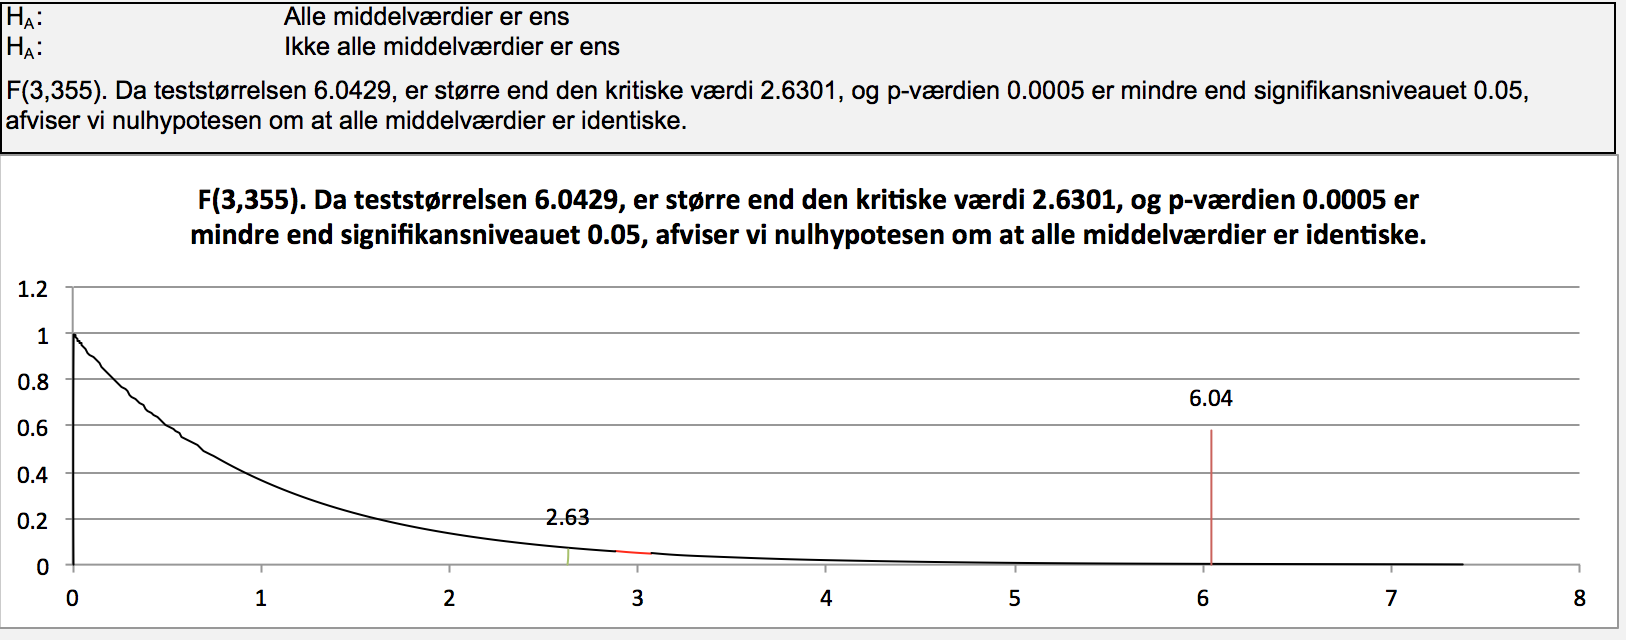
\includegraphics{img/anovaFtest.png}

Vi skal tjekke forudsætningen om varianshomogenitet

\[H_0:\sigma_{Design 1}=\sigma_{Design 2}=\sigma_{Design 3}=\sigma_{Design 4}\]\[H_1:Ikke\ alle\ varianser\ er\ ens\ for\ de\ 4\ designs.\]

Vi får en teststørrelse på 1.4742741. Chi i anden testet giver os en p-værdi på 0.6882205, hvilket er større end signifikanssandsynligheden på 0.05, vi kan ikke afvise nulhypotesen. Varianserne er ens, så forudsætningen er opfyldt.

Freestat output af Bartlett test for varianshomogenitet
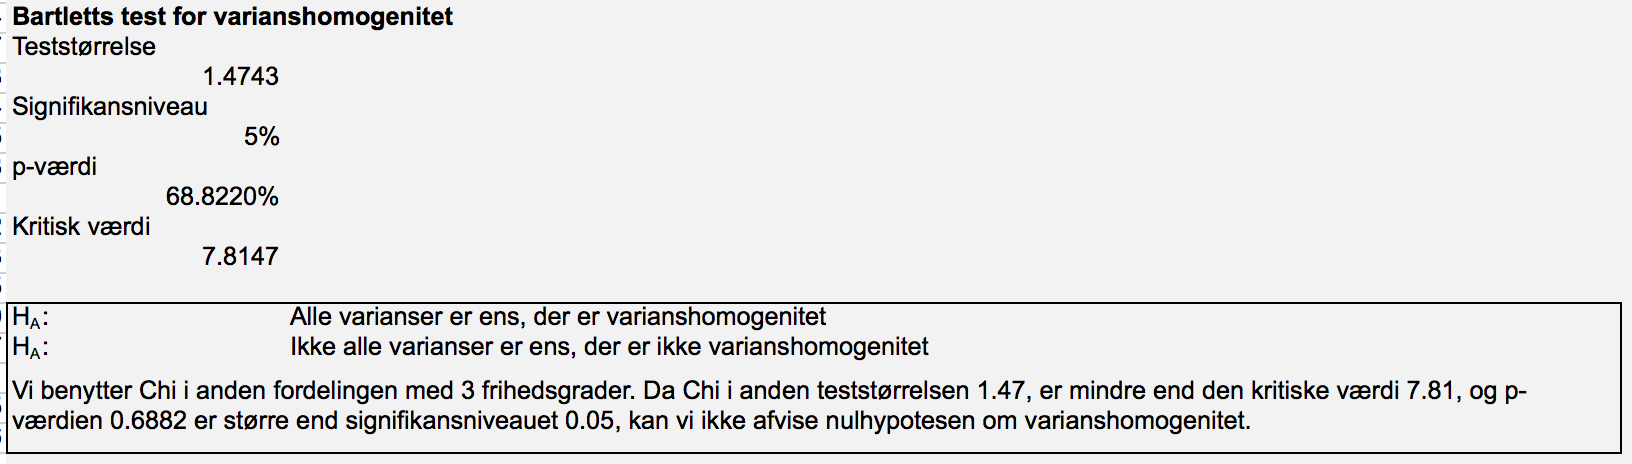
\includegraphics{img/Bartlett.png}

Normalitet

Herunder er 4 normalfraktildiagrammer, for de 4 designs, vi kan godt antage, stikprøverne stammer fra normalfordelte populationer.

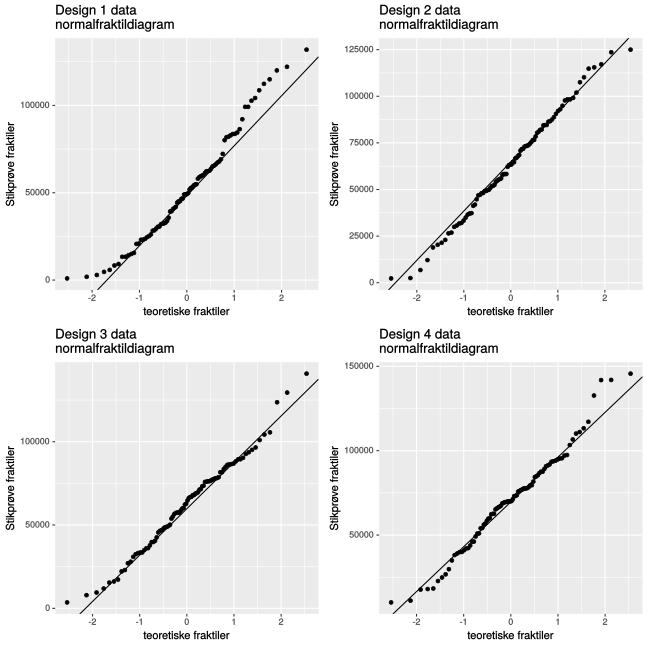
\includegraphics{_main_files/figure-latex/qqplots15_25-1.svg}

Tukey Kramer

Vi kan undersøge hvilke designs der har de største afvigelser ved at se på forskellene mellem stikprøvegennemsnittene, der er størst forskel mellem besøgstiderne for design 1 og design 4.

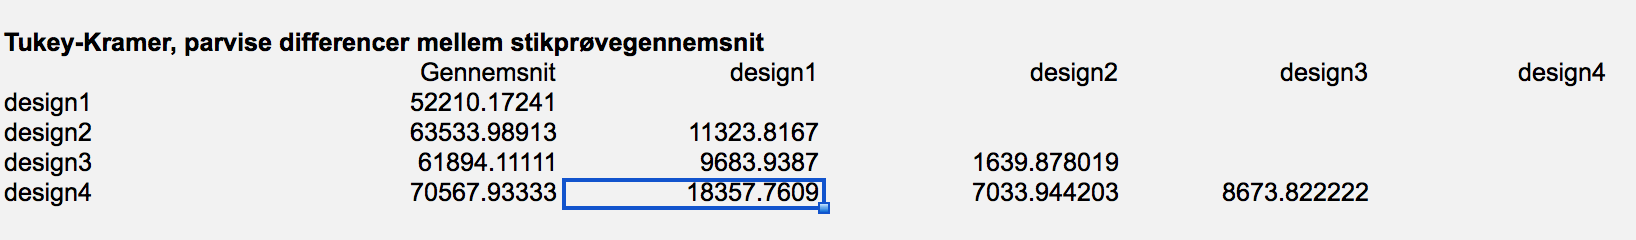
\includegraphics{img/Tukeykramer.png}

Vi kan grafisk sammenligne middelværdierne i boxplots, her ser vi ligeledes forskellen er størst mellem design 1 og design 4. Middelværdierne er markeret med orange prikker.

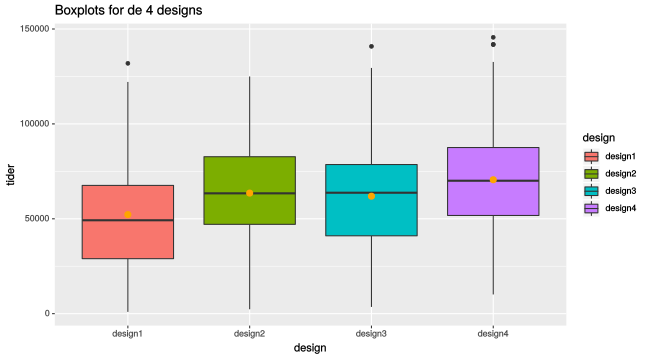
\includegraphics{_main_files/figure-latex/boxplots-1.svg}

Spørgsmål 3 banker afkast

Hent datasættet 3 Danske Banker Ugeafkast i procent
, i dette datasæt er de seneste 278 ugers afkast i procent for hhv. Danske Bank, Jyske Bank og Sydbank. Er der signifikant forskel på afkastene på de 3 bankaktier?

Svar 3 banker afkast
Vi opstiller hypoteserne for test af om middelværdierne er identiske:
\[H_0:\mu_{Danske Bank}=\mu_{Jyske Bank}=\mu_{Sydbank}\]\[H_1:Ikke\ alle\ middelvæ\ rdier\ er\ ens\ for\ de\ 3\ banker\]

Vi får variationen i grupperne SSW til 7878.1612 og variationen mellem grupperne SSA til 1.3759. Dette giver en F-teststørrelse på 0.0726 der resulterer i p-værdi på 0.93. Vi kan altså ikke forkaste altså nulhypotesen om ens middelværdier.

Vi kan da se at de absolutte forskelle mellem stikprøvegennemsnittene er relativt små:

\begin{longtable}[]{@{}ll@{}}
\toprule
Forskelle mellem Banker & Absolutte forskelle\tabularnewline
\midrule
\endhead
Danske Bank - Jyske Bank & 0.09\tabularnewline
Danske Bank - Sydbank & 0\tabularnewline
Jyske Bank - Sydbank & 0.08\tabularnewline
\bottomrule
\end{longtable}

Vi skal tjekke forudsætningen om varianshomogenitet

\[H_0:\sigma_{Danske Bank}=\sigma_{Jyske Bank}=\sigma_{Sydbank}\]\[H_1:Ikke\ alle\ varianser\ er\ ens\ for\ de\ 3\ banker.\]

Vi får en teststørrelse på 2.6184527. Chi i anden testet giver os en p-værdi på 0.2700289, hvilket er mindre end signifikanssandsynligheden på 0.05, vi afviser nulhypotesen. Varianserne er ikke ens, så forudsætningen er ikke opfyldt. Vi har således problemer med kvaliteten af analysen.

Normalitet

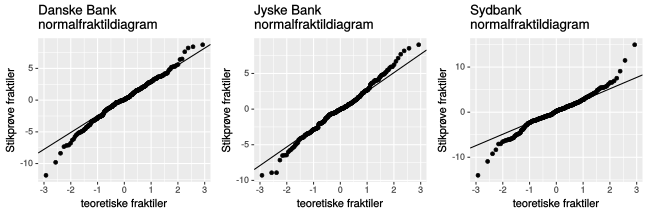
\includegraphics{_main_files/figure-latex/qqplotbank-1.svg}

Vi kan grafisk sammenligne middelværdierne for ugeafkastet for de 3 banker i boxplots , her ser vi der ikke er stor forskel på middelværdierne. Middelværdierne er markeret med orange prikker.

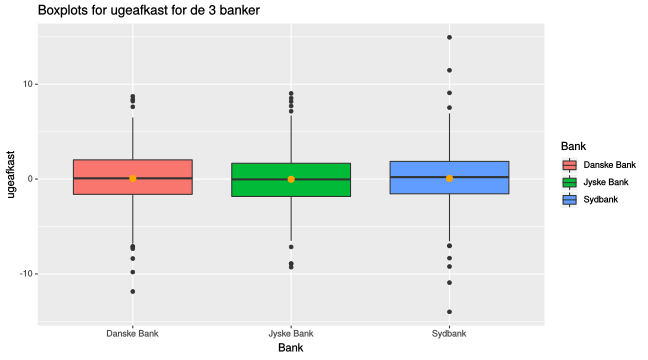
\includegraphics{_main_files/figure-latex/boxplotsbank-1.svg}

Spørgsmål IMDB

Hent IMDB data, der viser data for 759 film simpelt tilfældigt udtrukket af en database med 759 film. Vi ønsker at se om, der er forskel på vurderingen af de forskellige genrer action, komedie, drama, documentar, romance og short, undersøg dette vha. ANOVA test

Svar IMDB

Vi opstiller hypoteserne:

\[H_0:\mu_{action}=\mu_{komedie}=\mu_{drama}=\mu_{documentar}=\mu_{romance}=\mu_{short}\]\[H_1:Ikke\ alle\ middelvæ\ rdier\ er\ ens\ for\ de\ 5\ genrer.\]

Vi får en F-teststørrelse på 10.786, der resulterer i en meget lille p-værdi på 0, hvilket er klart under signifikansniveauet på 0.05. Vi kan forkaster altså nulhypotesen om ens middelværdier.

Vi skal tjekke forudsætningen om varianshomogenitet

\[H_0:\sigma_{action}=\sigma_{komedie}=\sigma_{drama}=\sigma_{documentar}=\sigma_{romance}=\sigma_{short}\]\[H_1:Ikke\ alle\ standardafvigelser\ er\ ens\ for\ de\ 5\ genrer.\]

Vi får en teststørrelse på 7.1306596. Chi i anden testet giver os en p-værdi på 0.2111029.

Normalitet

Herunder er 5 normalfraktildiagrammer, for de 5 genrer, dokumentar og short genrerne ser ikke normalfordelte ud. Hvilket kan give problemer med kvaliteten i vor analyse.

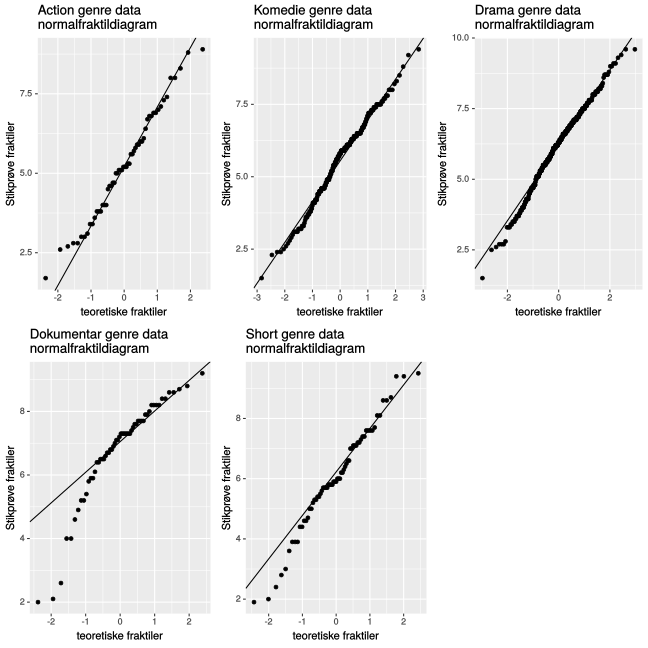
\includegraphics{_main_files/figure-latex/imdbqqplot-1.svg}

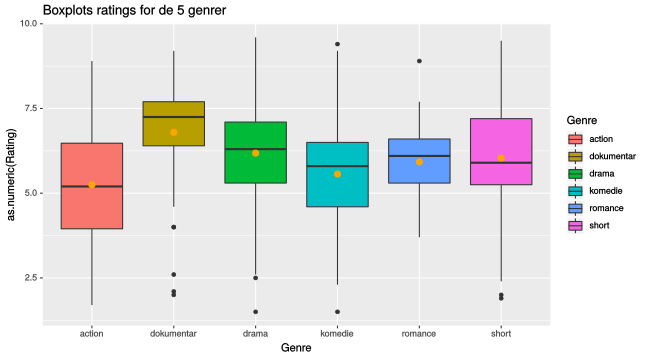
\includegraphics{_main_files/figure-latex/boxplotsimdb-1.svg}

Vi kan ud fra boxplots se at dokumentarfilm rates højt i modsætning til actionfilm. Vi kan i tabellen herunder se hvor de største forskelle er mellem genrerne.

\begin{longtable}[]{@{}ll@{}}
\toprule
Forskelle gennemsnit genrer & Absolutte forskelle\tabularnewline
\midrule
\endhead
Action - dokumentar & 1.5465517\tabularnewline
Action - drama & 0.9324561\tabularnewline
Action - komedie & 0.3148402\tabularnewline
Action - romance & 0.6735294\tabularnewline
Action - short & 0.788806\tabularnewline
Dokumentar - drama & 0.6140956\tabularnewline
Dokumentar - komedie & 1.2317115\tabularnewline
Dokumentar - romance & 0.8730223\tabularnewline
Dokumentar - short & 0.7577458\tabularnewline
Drama - komedie & 0.617616\tabularnewline
Drama - romance & 0.2589267\tabularnewline
Drama - short & 0.1436502\tabularnewline
Komedie - romance & 0.3586892\tabularnewline
Komedie - short & 0.4739658\tabularnewline
Romance - short & 0.1152766\tabularnewline
\bottomrule
\end{longtable}

\hypertarget{selvtest-2}{%
\section{Selvtest}\label{selvtest-2}}

Selvtest Anova analyse Realkredit med videoløsninger

\hypertarget{selvtest-3}{%
\section{Selvtest}\label{selvtest-3}}

Selvtest Anova analyse Aktier med videoløsninger

\hypertarget{cran-r}{%
\chapter{Cran R}\label{cran-r}}

\hypertarget{Sentry_noJS}{}
Sentry Page Protection

\hypertarget{Sentry_redirecting}{}
Please Wait\ldots{}

Vi bruger software programmet R da det er gratis og kan bruges til alt indenfor statistik, det er svært i begyndelsen, så sørg for at komme til timerne :O)

Der er et hav af videoer på youtube og hjælpesider fx.

\url{https://youtu.be/cX532N_XLIs?list=PLqzoL9-eJTNBDdKgJgJzaQcY6OXmsXAHU}

\url{https://youtu.be/UYclmg1_KLk?list=PLqzoL9-eJTNBDdKgJgJzaQcY6OXmsXAHU}

\url{https://youtu.be/2TcPAZOyV0U?list=PLqzoL9-eJTNBDdKgJgJzaQcY6OXmsXAHU}

\url{https://youtu.be/qPk0YEKhqB8?list=PLqzoL9-eJTNBDdKgJgJzaQcY6OXmsXAHU}

\url{https://youtu.be/3RWb5U3X-T8?list=PLqzoL9-eJTNBDdKgJgJzaQcY6OXmsXAHU}

\url{https://www.datacamp.com/courses/free-introduction-to-r}

\url{https://cran.r-project.org/doc/contrib/Paradis-rdebuts_en.pdf}

\url{http://dss.princeton.edu/training/RStudio101.pdf}

\url{https://youtu.be/uwlwNRbaKMI}

\hypertarget{r-video-tutorials}{%
\section{R video-tutorials}\label{r-video-tutorials}}

Herunder er 3 begynder videotutorials forsøg at gøre det samme som i videoerne. Du kan downloade scripts fra hver tutorial direkte under hver videovindue.

Hent r script klik her.

Hent r script klik her.

Hent r script klik her.

\hypertarget{faktoranalyse}{%
\chapter{Faktoranalyse}\label{faktoranalyse}}

\hypertarget{Sentry_noJS}{}
Sentry Page Protection

\hypertarget{Sentry_redirecting}{}
Please Wait\ldots{}

Faktoranalyse FA er ligesom, klyngeanalyse vi ser på senere, en strukturanalyse, der belyser hvilke sammenhænge der er i et datasæt. FA er en statistikmodel der navnlig bruges til at forenkle tolkningen af et datamateriale, der indeholder en stor mængde variable. FA bygger på et kæmpe antal udregninger med udgangspunkt i korrelationskoefficienter og er i praksis nærmest umulig at gennemføre uden brug af computersoftware. Før computerens opfindelse kunne en faktoranalyse nemt lægge beslag på en halv snes statistikere på fuld tid gennem flere måneder. Resultatet ville være identifikation få faktorer, skjult i et datamateriale.

Faktoranalysen kan fx. hjælpe med at vise sammenhænge mellem svar i spørgeskemaer, hvilket kan være en hjælp markedsføringsmæssigt, til at forstå hvilke svar samvarierer. En sådan gruppering af spørgsmål kan hjælpe med bedre at forstå kundernes ønsker og behov. Faktoranalyse FA er et godt værktøj til at forstå, hvad dine spørgeskemadata betyder, især når du har mange variable. Faktoranalysen forsøger at finde skjulte variable, som forklarer opførslen af dine observerede variable. FA har historiske rødder i psykometri, dvs målingen af mentale egenskaber.

I modsætning hertil søger man med Klyngeanalysen at finde sammenhænge mellem respondenterne/observationerne og altså ikke variablene, hvilket er et godt hjælpeværktøj i forbindelse med markedssegmentering.

Der findes 2 typer af FA Exploratory Factor Analysis (EFA) og Confirmatory Factor Analysis (CFA). EFA betyder, at du ikke rigtig ved, hvilke skjulte variable (eller faktorer) der findes, og hvor mange de er, så du forsøger at finde dem. CFA betyder, at du allerede har nogle gæt eller modeller på skjulte variable (eller faktorer), og vi vil kontrollere, om dette er korrekt. Vi benytter i det følgende EFA

\hypertarget{hvilke-faktorer-er-vigtige-nar-man-kber-en-ny-computer}{%
\section{Hvilke faktorer er vigtige når man køber en ny computer:}\label{hvilke-faktorer-er-vigtige-nar-man-kber-en-ny-computer}}

Lad os sige, man har indsamlet et spørgeskema for at undersøge, hvad der er vigtigt, når en forbruger bestemmer, hvilken computer der skal købes. Spørgeskemaet er udformet, som hvor vigtig er Pris for computerkøbet, vægt fra 1 til 7 hvor 7 er højest/vigtigst.

Dette datasæt er lille i forhold til, hvad der er realistisk, da vi blot forsøger at illustrere analysen. Normalt vil man have flere end 6 variable. For at sikre solide analyseresultater, vil man ligeledes have flere respondenter/observationer.

I noterne er input til R og output fra R, markeret i grå rammer. Output dvs. resultaterne R leverer er markeret med \#\# i hver linje. Input dvs. de kommandoer vi skal skrive ind i R er ikke markeret.

Rammen herunder er input til R, da linjerne ikke er markeret. Læs datasættet ind i R, dette kan du gøre ved at copy paste nedenstående kode, i den grå ramme, direkte ind i R enten i console eller et script.

Bemærk data.frame er en to-dimensionel data struktur, nedenstående betyder vore 6 variable nu er lagret i en dataframe.

\begin{Shaded}
\begin{Highlighting}[]
\NormalTok{Pris <-}\StringTok{ }\KeywordTok{c}\NormalTok{(}\DecValTok{6}\NormalTok{,}\DecValTok{7}\NormalTok{,}\DecValTok{6}\NormalTok{,}\DecValTok{5}\NormalTok{,}\DecValTok{7}\NormalTok{,}\DecValTok{6}\NormalTok{,}\DecValTok{5}\NormalTok{,}\DecValTok{6}\NormalTok{,}\DecValTok{3}\NormalTok{,}\DecValTok{1}\NormalTok{,}\DecValTok{2}\NormalTok{,}\DecValTok{5}\NormalTok{,}\DecValTok{2}\NormalTok{,}\DecValTok{3}\NormalTok{,}\DecValTok{1}\NormalTok{,}\DecValTok{2}\NormalTok{)}
\NormalTok{Software <-}\StringTok{ }\KeywordTok{c}\NormalTok{(}\DecValTok{5}\NormalTok{,}\DecValTok{3}\NormalTok{,}\DecValTok{4}\NormalTok{,}\DecValTok{7}\NormalTok{,}\DecValTok{7}\NormalTok{,}\DecValTok{4}\NormalTok{,}\DecValTok{7}\NormalTok{,}\DecValTok{5}\NormalTok{,}\DecValTok{5}\NormalTok{,}\DecValTok{3}\NormalTok{,}\DecValTok{6}\NormalTok{,}\DecValTok{7}\NormalTok{,}\DecValTok{4}\NormalTok{,}\DecValTok{5}\NormalTok{,}\DecValTok{6}\NormalTok{,}\DecValTok{3}\NormalTok{)}
\NormalTok{Æstetik <-}\StringTok{ }\KeywordTok{c}\NormalTok{(}\DecValTok{3}\NormalTok{,}\DecValTok{2}\NormalTok{,}\DecValTok{4}\NormalTok{,}\DecValTok{1}\NormalTok{,}\DecValTok{5}\NormalTok{,}\DecValTok{2}\NormalTok{,}\DecValTok{2}\NormalTok{,}\DecValTok{4}\NormalTok{,}\DecValTok{6}\NormalTok{,}\DecValTok{7}\NormalTok{,}\DecValTok{6}\NormalTok{,}\DecValTok{7}\NormalTok{,}\DecValTok{5}\NormalTok{,}\DecValTok{6}\NormalTok{,}\DecValTok{5}\NormalTok{,}\DecValTok{7}\NormalTok{)}
\NormalTok{Brand <-}\StringTok{ }\KeywordTok{c}\NormalTok{(}\DecValTok{4}\NormalTok{,}\DecValTok{2}\NormalTok{,}\DecValTok{5}\NormalTok{,}\DecValTok{3}\NormalTok{,}\DecValTok{5}\NormalTok{,}\DecValTok{3}\NormalTok{,}\DecValTok{1}\NormalTok{,}\DecValTok{4}\NormalTok{,}\DecValTok{7}\NormalTok{,}\DecValTok{5}\NormalTok{,}\DecValTok{7}\NormalTok{,}\DecValTok{6}\NormalTok{,}\DecValTok{6}\NormalTok{,}\DecValTok{5}\NormalTok{,}\DecValTok{5}\NormalTok{,}\DecValTok{7}\NormalTok{)}
\NormalTok{Venner <-}\StringTok{ }\KeywordTok{c}\NormalTok{(}\DecValTok{7}\NormalTok{,}\DecValTok{2}\NormalTok{,}\DecValTok{5}\NormalTok{,}\DecValTok{6}\NormalTok{,}\DecValTok{2}\NormalTok{,}\DecValTok{4}\NormalTok{,}\DecValTok{1}\NormalTok{,}\DecValTok{7}\NormalTok{,}\DecValTok{3}\NormalTok{,}\DecValTok{2}\NormalTok{,}\DecValTok{6}\NormalTok{,}\DecValTok{7}\NormalTok{,}\DecValTok{6}\NormalTok{,}\DecValTok{2}\NormalTok{,}\DecValTok{4}\NormalTok{,}\DecValTok{5}\NormalTok{)}
\NormalTok{Familie <-}\StringTok{ }\KeywordTok{c}\NormalTok{(}\DecValTok{6}\NormalTok{,}\DecValTok{3}\NormalTok{,}\DecValTok{4}\NormalTok{,}\DecValTok{7}\NormalTok{,}\DecValTok{1}\NormalTok{,}\DecValTok{5}\NormalTok{,}\DecValTok{4}\NormalTok{,}\DecValTok{5}\NormalTok{,}\DecValTok{4}\NormalTok{,}\DecValTok{4}\NormalTok{,}\DecValTok{5}\NormalTok{,}\DecValTok{7}\NormalTok{,}\DecValTok{2}\NormalTok{,}\DecValTok{3}\NormalTok{,}\DecValTok{5}\NormalTok{,}\DecValTok{6}\NormalTok{)}

\NormalTok{data <-}\StringTok{ }\KeywordTok{data.frame}\NormalTok{(Pris, Software, Æstetik, Brand, Venner, Familie)}
\end{Highlighting}
\end{Shaded}

\hypertarget{forudstninger-for-faktoranalysen.}{%
\section{Forudsætninger for faktoranalysen.}\label{forudstninger-for-faktoranalysen.}}

Nu skal vi undersøge om det er fornuftigt at foretage en faktoranalyse, dette kan vi undersøge ved enten Bartletts korrelationstest eller Kaiser-Meyer-Olkin KMO.

For at teste dette skal man installere og loade pakken psych, vi skal kun installere første gang. Bemærk install.packages(``psych'') er kommenteret ud nedenfor, så første gang skal du kommentere install.packages(``psych'') ud.

\begin{Shaded}
\begin{Highlighting}[]
\CommentTok{#install.packages("psych")}
\KeywordTok{library}\NormalTok{(}\StringTok{"psych"}\NormalTok{)}
\end{Highlighting}
\end{Shaded}

Du kan alternativt benytte pacman pakken, hvilket ofte er at foretrække. Hvis du indlæser nedenstående installeres og loades pakken psych:

\begin{Shaded}
\begin{Highlighting}[]
\ControlFlowTok{if}\NormalTok{ (}\OperatorTok{!}\KeywordTok{require}\NormalTok{(}\StringTok{"pacman"}\NormalTok{)) }\KeywordTok{install.packages}\NormalTok{(}\StringTok{"pacman"}\NormalTok{)}
\NormalTok{pacman}\OperatorTok{::}\KeywordTok{p_load}\NormalTok{(psych)}
\end{Highlighting}
\end{Shaded}

Nu hvor psych pakken er indlæst kan vi køre Bartletts test i R:

\begin{Shaded}
\begin{Highlighting}[]
\KeywordTok{cortest.bartlett}\NormalTok{(data)}
\end{Highlighting}
\end{Shaded}

\begin{verbatim}
## $chisq
## [1] 36.15696
## 
## $p.value
## [1] 0.00167791
## 
## $df
## [1] 15
\end{verbatim}

Nulhypotesen i Bartletts test er at variablene ikke er korrelerede dvs. alle korrelationskoefficienter \(\rho=0\),

\[H_0:Alle\ \rho=0\]
\[H_1:Ikke\ alle\ \rho=0  \]

Forkaster vi nulhypotesen, er der basis for at gennemføre faktoranalysen. Den lille p-værdi på 0.00167791, betyder vi gennemfører faktoranalysen.

Vi kan ligeledes køre Kaiser-Meyer-Olkin KMO testet fra pshych pakken:

\begin{Shaded}
\begin{Highlighting}[]
\KeywordTok{KMO}\NormalTok{(data)}
\end{Highlighting}
\end{Shaded}

\begin{verbatim}
## Kaiser-Meyer-Olkin factor adequacy
## Call: KMO(r = data)
## Overall MSA =  0.49
## MSA for each item = 
##     Pris Software  Æstetik    Brand   Venner  Familie 
##     0.71     0.70     0.57     0.49     0.30     0.37
\end{verbatim}

For KMO skal Overall MSA = 0.49, fortæller om egnethed af data til faktoranalyse. Skal være større end kritisk grænse på ca. 0.5, dette er ikke helt tilfældet her, men vi gennemfører alligevel faktoranalysen.

Vi kan se af korrelationsmatricen, at nogle variable er korrellerede og andre tilsyneladende ikke.

\begin{Shaded}
\begin{Highlighting}[]
\KeywordTok{cor}\NormalTok{(data)}
\end{Highlighting}
\end{Shaded}

\begin{verbatim}
##                 Pris   Software     Æstetik       Brand     Venner
## Pris      1.00000000  0.1856123 -0.63202219 -0.58026680 0.03082006
## Software  0.18561230  1.0000000 -0.14621516 -0.11858645 0.10096774
## Æstetik  -0.63202219 -0.1462152  1.00000000  0.85285436 0.03989799
## Brand    -0.58026680 -0.1185864  0.85285436  1.00000000 0.33316719
## Venner    0.03082006  0.1009677  0.03989799  0.33316719 1.00000000
## Familie  -0.06183118  0.1765724 -0.06977360  0.02662389 0.60727189
##              Familie
## Pris     -0.06183118
## Software  0.17657236
## Æstetik  -0.06977360
## Brand     0.02662389
## Venner    0.60727189
## Familie   1.00000000
\end{verbatim}

Så det ser ud til, at Pris har stærke negative sammenhænge med Æstetik og Brand.
Venner har en stærk positiv sammenhæng med Familie.

Det betyder, at vi kan forvente, at vi vil have to fælles faktorer, og en vil være relateret til pris, æstetik og brand, og den anden vil være relateret til ven og familie. Vi kan lave et corrplot, der grafisk illustrerer disse sammenhænge, store blå prikker er positiv korrelation, store røde negativ korrelation. Så vi skal installere corplott pakken, her bruger vi pacman til installationen.

\begin{Shaded}
\begin{Highlighting}[]
\NormalTok{pacman}\OperatorTok{::}\KeywordTok{p_load}\NormalTok{(corrplot)}
\KeywordTok{corrplot}\NormalTok{(}\KeywordTok{cor}\NormalTok{(data), }\DataTypeTok{order =} \StringTok{"hclust"}\NormalTok{, }\DataTypeTok{tl.col=}\StringTok{'black'}\NormalTok{, }\DataTypeTok{tl.cex=}\NormalTok{.}\DecValTok{5}\NormalTok{)}
\end{Highlighting}
\end{Shaded}

\includegraphics{_main_files/figure-latex/corrplot-1.svg}

\hypertarget{selve-faktoranalysen}{%
\section{Selve Faktoranalysen}\label{selve-faktoranalysen}}

Vi er nu klar til at teste om der er grundlag for at sammenlægge variable til faktorer. Dette tester vi i selve faktor analysen, ved hjælp af funktionen factanal.

Hvis vi samler alle spørgsmål til en samlet faktor, har vi følgende faktor analyse:

\begin{Shaded}
\begin{Highlighting}[]
\NormalTok{fa1 <-}\StringTok{ }\KeywordTok{factanal}\NormalTok{(data, }\DataTypeTok{factor=}\DecValTok{1}\NormalTok{)}
\NormalTok{fa1}
\end{Highlighting}
\end{Shaded}

\begin{verbatim}
## 
## Call:
## factanal(x = data, factors = 1)
## 
## Uniquenesses:
##     Pris Software  Æstetik    Brand   Venner  Familie 
##    0.567    0.977    0.126    0.167    0.974    1.000 
## 
## Loadings:
##          Factor1
## Pris     -0.658 
## Software -0.152 
## Æstetik   0.935 
## Brand     0.912 
## Venner    0.161 
## Familie         
## 
##                Factor1
## SS loadings      2.190
## Proportion Var   0.365
## 
## Test of the hypothesis that 1 factor is sufficient.
## The chi square statistic is 12.79 on 9 degrees of freedom.
## The p-value is 0.172
\end{verbatim}

\textbf{Uniqueness} angiver hvor meget af variationen i en variabel, der ikke er associeret med faktoren. Jo lavere Uniqueness, des større sammenhæng til faktorerne.

\textbf{Loadings} angiver hvordan hver variabel er vægtet for faktorerne, men også hvor stærk korrelationen er til hver faktor. Faktor 1 påvirkes således mest af Æstetik, Brand og Pris. Denne faktor kan ses af corrplottet hvor disse tre variable ses at påvirke hinanden, Pris er negativt korreleret med Æstetik og Brand.

\textbf{Proportion Var} er et vigtigt nøgletal, der angiver andelen af variationen i data, der er forklaret af den pågældende faktor. Her forklares alså kun 36.5\% af variationen i datasættet. Proportion Var findes som SS loadings divideret med antallet af variable dvs. her 6.

Lad os se på hvad der sker, hvis vi deler variablene op i 2 faktorer:

\begin{Shaded}
\begin{Highlighting}[]
\NormalTok{fa2 <-}\StringTok{ }\KeywordTok{factanal}\NormalTok{(data, }\DataTypeTok{factor=}\DecValTok{2}\NormalTok{)}
\NormalTok{fa2}
\end{Highlighting}
\end{Shaded}

\begin{verbatim}
## 
## Call:
## factanal(x = data, factors = 2)
## 
## Uniquenesses:
##     Pris Software  Æstetik    Brand   Venner  Familie 
##    0.559    0.960    0.126    0.080    0.005    0.609 
## 
## Loadings:
##          Factor1 Factor2
## Pris     -0.657         
## Software -0.161   0.119 
## Æstetik   0.933         
## Brand     0.928   0.242 
## Venner    0.100   0.992 
## Familie           0.620 
## 
##                Factor1 Factor2
## SS loadings      2.207   1.453
## Proportion Var   0.368   0.242
## Cumulative Var   0.368   0.610
## 
## Test of the hypothesis that 2 factors are sufficient.
## The chi square statistic is 2.16 on 4 degrees of freedom.
## The p-value is 0.706
\end{verbatim}

\textbf{Cumulative Var} 0.61 er summen af proportion var 0.368 og 0.242, og betyder at faktor 1 og faktor 2 forklarer 61\% af variationen i datamaterialet.

Faktor 2 forklares altså primært af Venner og Familie, dette stemmer godt overens med billedet vi så i corrplot.

Nu opdeler vi variablene i 3 faktorer.

\begin{Shaded}
\begin{Highlighting}[]
\NormalTok{fa3 <-}\StringTok{ }\KeywordTok{factanal}\NormalTok{(data, }\DataTypeTok{factor=}\DecValTok{3}\NormalTok{)}
\NormalTok{fa3}
\end{Highlighting}
\end{Shaded}

\begin{verbatim}
## 
## Call:
## factanal(x = data, factors = 3)
## 
## Uniquenesses:
##     Pris Software  Æstetik    Brand   Venner  Familie 
##    0.468    0.944    0.154    0.005    0.193    0.005 
## 
## Loadings:
##          Factor1 Factor2 Factor3
## Pris     -0.717           0.122 
## Software -0.146   0.172         
## Æstetik   0.908  -0.130         
## Brand     0.892  -0.116   0.430 
## Venner            0.440   0.781 
## Familie           0.970   0.228 
## 
##                Factor1 Factor2 Factor3
## SS loadings      2.161   1.198   0.872
## Proportion Var   0.360   0.200   0.145
## Cumulative Var   0.360   0.560   0.705
## 
## The degrees of freedom for the model is 0 and the fit was 0.0188
\end{verbatim}

Nu forklares 70.5\% af variationen i datamaterialet altså ud fra de 3 faktorer.

\hypertarget{hvor-mange-faktorer-br-benyttes}{%
\section{Hvor mange faktorer bør benyttes?}\label{hvor-mange-faktorer-br-benyttes}}

Der er ingen fast regel for hvor mange faktorer der bør benyttes. Der er flere forskelle metoder til bestemmelse af antallet af faktorer, vi viser herunder 2 metoder.

\hypertarget{eigenvalues-metoden}{%
\subsection{Eigenvalues metoden}\label{eigenvalues-metoden}}

Eigenvalues udtrykker hvor meget af datamaterialets samlede varians, der dækkes af den pågældende faktor. Eigenvalues er standardiserede således at summen giver antallet af variable, herunder ses at summen er 6, da der er 6 variable i datasættet. Vi ser hvor stor en del af variationen hver faktor forklarer, når der er 6 faktorer. Faktor 5 og faktor 6 bibringer meget lidt yderligere forklaring af variationen.

\begin{Shaded}
\begin{Highlighting}[]
\NormalTok{ev <-}\StringTok{ }\KeywordTok{eigen}\NormalTok{(}\KeywordTok{cor}\NormalTok{(data))}
\NormalTok{ev}\OperatorTok{$}\NormalTok{values}
\end{Highlighting}
\end{Shaded}

\begin{verbatim}
## [1] 2.45701130 1.68900056 0.89157047 0.60583326 0.27285334 0.08373107
\end{verbatim}

\begin{Shaded}
\begin{Highlighting}[]
\KeywordTok{sum}\NormalTok{(ev}\OperatorTok{$}\NormalTok{values)}
\end{Highlighting}
\end{Shaded}

\begin{verbatim}
## [1] 6
\end{verbatim}

\begin{Shaded}
\begin{Highlighting}[]
\NormalTok{ev}\OperatorTok{$}\NormalTok{values}\OperatorTok{/}\KeywordTok{sum}\NormalTok{(ev}\OperatorTok{$}\NormalTok{values)}
\end{Highlighting}
\end{Shaded}

\begin{verbatim}
## [1] 0.40950188 0.28150009 0.14859508 0.10097221 0.04547556 0.01395518
\end{verbatim}

Når vi benytter Eigenvalues metoden, bestemmes antallet af faktorer ud fra antallet af Eigenvalues større end 1, det er denne metode fx. SPSS benytter. Vi ser at kun 2 Eigenvalues er 2.45701130 og 1.68900056 er større end 1, vi får således kun 2 faktorer. Eigenvalues metoden er ofte lidt konservativ, således at vi får færre faktorer end med de øvrige metoder.

\hypertarget{screeplot-metoden}{%
\subsection{Screeplot metoden}\label{screeplot-metoden}}

Vi kan se på nedenstående screeplot, der hvor kurven flader ud, bibringer yderligere faktorer ikke synderlig megen yderligere forklaring til modellen. Man vil med screeplot kriteriet, vælge antallet af faktorer hvor kurven knækkker i tilfældet med 3 faktorer. Man vil ikke altid entydigt kunne afgøre hvor screeplot kurven knækker, her må man så afgøre dette bedst muligt.

\begin{Shaded}
\begin{Highlighting}[]
\KeywordTok{screeplot}\NormalTok{(}\KeywordTok{princomp}\NormalTok{(data),}\DataTypeTok{type=}\StringTok{"line"}\NormalTok{,}\DataTypeTok{npcs =} \DecValTok{6}\NormalTok{, }\DataTypeTok{main=}\StringTok{"Screeplot Computereksempel"}\NormalTok{)}
\end{Highlighting}
\end{Shaded}

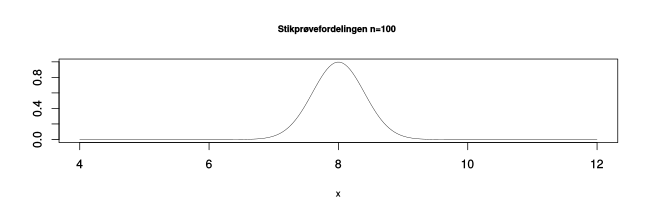
\includegraphics{_main_files/figure-latex/unnamed-chunk-13-1.svg}

Spørgsmål personality Stanford
Hent nu filen personality, hvor 240 Stanford studerende har svaret på i hvor høj grad de mener at besidde 32 forskellige personlighedstræk. 1 til 8 hvor 1 er mindst og 8 er mest. Foretag hvis en test viser dette er fordelagtigt en faktoranalyse.

Download personality fra filen her og importer den i R via File - Import Dataset.

Svar personality Stanford

\begin{Shaded}
\begin{Highlighting}[]
\NormalTok{pacman}\OperatorTok{::}\KeywordTok{p_load}\NormalTok{(psych)}
\KeywordTok{cortest.bartlett}\NormalTok{(personality)}
\end{Highlighting}
\end{Shaded}

\begin{verbatim}
## R was not square, finding R from data
\end{verbatim}

\begin{verbatim}
## $chisq
## [1] 4009.545
## 
## $p.value
## [1] 0
## 
## $df
## [1] 496
\end{verbatim}

\begin{Shaded}
\begin{Highlighting}[]
\KeywordTok{KMO}\NormalTok{(personality)}
\end{Highlighting}
\end{Shaded}

\begin{verbatim}
## Kaiser-Meyer-Olkin factor adequacy
## Call: KMO(r = personality)
## Overall MSA =  0.84
## MSA for each item = 
## distant talkatv carelss hardwrk anxious agreebl   tense    kind opposng 
##    0.88    0.86    0.82    0.87    0.82    0.73    0.84    0.81    0.79 
## relaxed disorgn outgoin approvn     shy discipl   harsh persevr friendl 
##    0.86    0.75    0.87    0.89    0.87    0.84    0.85    0.86    0.87 
## worryin respnsi contrar sociabl    lazy coopera   quiet organiz criticl 
##    0.81    0.86    0.83    0.90    0.89    0.83    0.87    0.78    0.87 
##     lax laidbck withdrw givinup easygon 
##    0.81    0.73    0.90    0.89    0.78
\end{verbatim}

Vi gennemfører klart analysen viser begge tests.

\begin{Shaded}
\begin{Highlighting}[]
\CommentTok{#cor(personality) korrelationsmatricen er udeladt af pladshensyn.}
\KeywordTok{corrplot}\NormalTok{(}\KeywordTok{cor}\NormalTok{(personality), }\DataTypeTok{order =} \StringTok{"hclust"}\NormalTok{, }\DataTypeTok{tl.col=}\StringTok{'black'}\NormalTok{, }\DataTypeTok{tl.cex=}\NormalTok{.}\DecValTok{5}\NormalTok{)}
\end{Highlighting}
\end{Shaded}

\includegraphics{_main_files/figure-latex/unnamed-chunk-16-1.svg}

\begin{Shaded}
\begin{Highlighting}[]
\KeywordTok{screeplot}\NormalTok{(}\KeywordTok{princomp}\NormalTok{(personality),}\DataTypeTok{type=}\StringTok{"line"}\NormalTok{, }\DataTypeTok{main=}\StringTok{"Screeplot personality"}\NormalTok{)}
\end{Highlighting}
\end{Shaded}

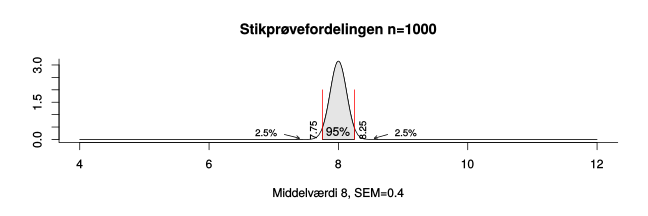
\includegraphics{_main_files/figure-latex/unnamed-chunk-17-1.svg}

\begin{Shaded}
\begin{Highlighting}[]
\NormalTok{evp <-}\StringTok{ }\KeywordTok{eigen}\NormalTok{(}\KeywordTok{cor}\NormalTok{(personality))}
\NormalTok{evp}\OperatorTok{$}\NormalTok{values}
\end{Highlighting}
\end{Shaded}

\begin{verbatim}
##  [1] 7.2407068 4.5250901 3.1240573 2.3335890 1.8783611 1.1940636 0.9268636
##  [8] 0.8553802 0.7968460 0.7128793 0.6936229 0.6396893 0.6277046 0.5399600
## [15] 0.5074253 0.4719721 0.4639916 0.4455816 0.4376430 0.4135706 0.3906941
## [22] 0.3696839 0.3273829 0.3014077 0.2940833 0.2800131 0.2522101 0.2349649
## [29] 0.2199461 0.2011492 0.1658493 0.1336176
\end{verbatim}

Vi benytter her 7 faktorer:

\begin{Shaded}
\begin{Highlighting}[]
\NormalTok{fapers7 <-}\StringTok{ }\KeywordTok{factanal}\NormalTok{(personality,}\DecValTok{7}\NormalTok{)}
\NormalTok{fapers7}
\end{Highlighting}
\end{Shaded}

\begin{verbatim}
## 
## Call:
## factanal(x = personality, factors = 7)
## 
## Uniquenesses:
## distant talkatv carelss hardwrk anxious agreebl   tense    kind opposng 
##   0.529   0.377   0.491   0.416   0.347   0.576   0.273   0.416   0.512 
## relaxed disorgn outgoin approvn     shy discipl   harsh persevr friendl 
##   0.390   0.181   0.251   0.640   0.387   0.478   0.517   0.560   0.377 
## worryin respnsi contrar sociabl    lazy coopera   quiet organiz criticl 
##   0.388   0.411   0.392   0.367   0.421   0.528   0.284   0.229   0.562 
##     lax laidbck withdrw givinup easygon 
##   0.663   0.248   0.362   0.557   0.549 
## 
## Loadings:
##         Factor1 Factor2 Factor3 Factor4 Factor5 Factor6 Factor7
## distant  0.586           0.121  -0.172   0.246   0.137         
## talkatv -0.760                           0.144   0.105         
## carelss         -0.280   0.137  -0.134   0.192   0.586   0.111 
## hardwrk -0.182   0.700   0.141                  -0.187         
## anxious  0.153           0.774           0.136                 
## agreebl                          0.577  -0.194           0.212 
## tense    0.150           0.787           0.208          -0.179 
## kind    -0.102   0.188           0.699  -0.118  -0.189         
## opposng                         -0.115   0.672                 
## relaxed         -0.104  -0.526   0.263                   0.491 
## disorgn         -0.340                           0.830         
## outgoin -0.834   0.107           0.166                   0.113 
## approvn -0.284   0.137           0.438  -0.142           0.214 
## shy      0.724  -0.240   0.153                                 
## discipl          0.698                          -0.164         
## harsh                           -0.265   0.619   0.132         
## persevr -0.134   0.598           0.216                         
## friendl -0.504   0.129           0.571  -0.131                 
## worryin  0.163           0.722           0.119          -0.216 
## respnsi          0.578           0.331          -0.343  -0.152 
## contrar                  0.159  -0.162   0.730   0.120         
## sociabl -0.733                   0.263                         
## lazy     0.167  -0.664   0.152           0.163   0.208   0.130 
## coopera          0.136  -0.123   0.603  -0.248                 
## quiet    0.789  -0.157   0.191   0.173                         
## organiz          0.433                          -0.753         
## criticl          0.112   0.124           0.614  -0.122         
## lax             -0.355           0.102           0.227   0.377 
## laidbck         -0.102  -0.288                   0.109   0.801 
## withdrw  0.720           0.172  -0.150   0.224   0.105         
## givinup  0.337  -0.438   0.280  -0.165   0.136   0.115         
## easygon -0.159  -0.116  -0.245   0.302                   0.508 
## 
##                Factor1 Factor2 Factor3 Factor4 Factor5 Factor6 Factor7
## SS loadings      4.501   3.076   2.494   2.403   2.221   2.068   1.560
## Proportion Var   0.141   0.096   0.078   0.075   0.069   0.065   0.049
## Cumulative Var   0.141   0.237   0.315   0.390   0.459   0.524   0.573
## 
## Test of the hypothesis that 7 factors are sufficient.
## The chi square statistic is 460.58 on 293 degrees of freedom.
## The p-value is 0.00000000137
\end{verbatim}

Vi benytter her 8 faktorer:

\begin{Shaded}
\begin{Highlighting}[]
\NormalTok{fapers8 <-}\StringTok{ }\KeywordTok{factanal}\NormalTok{(personality,}\DecValTok{8}\NormalTok{)}
\NormalTok{fapers8}
\end{Highlighting}
\end{Shaded}

\begin{verbatim}
## 
## Call:
## factanal(x = personality, factors = 8)
## 
## Uniquenesses:
## distant talkatv carelss hardwrk anxious agreebl   tense    kind opposng 
##   0.534   0.375   0.484   0.425   0.342   0.204   0.263   0.439   0.533 
## relaxed disorgn outgoin approvn     shy discipl   harsh persevr friendl 
##   0.417   0.170   0.257   0.649   0.364   0.490   0.468   0.497   0.333 
## worryin respnsi contrar sociabl    lazy coopera   quiet organiz criticl 
##   0.347   0.420   0.391   0.365   0.420   0.502   0.276   0.236   0.565 
##     lax laidbck withdrw givinup easygon 
##   0.682   0.005   0.367   0.550   0.580 
## 
## Loadings:
##         Factor1 Factor2 Factor3 Factor4 Factor5 Factor6 Factor7 Factor8
## distant  0.587           0.103  -0.118   0.262   0.134                 
## talkatv -0.761                           0.152   0.104                 
## carelss         -0.307   0.115           0.218   0.584          -0.108 
## hardwrk -0.182   0.694   0.139                  -0.188                 
## anxious  0.149           0.772           0.144                         
## agreebl                          0.795  -0.173           0.140  -0.327 
## tense    0.150           0.796           0.211          -0.152         
## kind    -0.118   0.227           0.615  -0.151  -0.182           0.238 
## opposng                  0.102  -0.116   0.654                         
## relaxed         -0.108  -0.535   0.276                   0.441         
## disorgn         -0.336                           0.836                 
## outgoin -0.836   0.107           0.147                                 
## approvn -0.294   0.129           0.445  -0.135           0.163         
## shy      0.729  -0.224   0.161                                   0.153 
## discipl          0.677                          -0.168          -0.105 
## harsh                           -0.178   0.658   0.124          -0.195 
## persevr -0.133   0.644           0.127                           0.206 
## friendl -0.517   0.170           0.471  -0.160                   0.326 
## worryin  0.164           0.744           0.101          -0.170   0.177 
## respnsi          0.599           0.285          -0.337  -0.117   0.105 
## contrar                  0.153  -0.152   0.732   0.118                 
## sociabl -0.737                   0.222                   0.104   0.123 
## lazy     0.166  -0.665   0.142           0.166   0.208   0.116         
## coopera -0.112   0.143  -0.130   0.614  -0.252                         
## quiet    0.789  -0.147   0.195   0.169                           0.109 
## organiz          0.434                          -0.748                 
## criticl          0.124   0.132           0.604  -0.119                 
## lax             -0.361           0.107           0.231   0.323         
## laidbck                 -0.277                   0.105   0.942         
## withdrw  0.721           0.152  -0.111   0.241   0.101                 
## givinup  0.337  -0.465   0.254  -0.106   0.161   0.108                 
## easygon -0.169  -0.117  -0.261   0.284                   0.467         
## 
##                Factor1 Factor2 Factor3 Factor4 Factor5 Factor6 Factor7
## SS loadings      4.549   3.181   2.531   2.325   2.287   2.052   1.583
## Proportion Var   0.142   0.099   0.079   0.073   0.071   0.064   0.049
## Cumulative Var   0.142   0.242   0.321   0.393   0.465   0.529   0.578
##                Factor8
## SS loadings      0.539
## Proportion Var   0.017
## Cumulative Var   0.595
## 
## Test of the hypothesis that 8 factors are sufficient.
## The chi square statistic is 398.53 on 268 degrees of freedom.
## The p-value is 0.000000379
\end{verbatim}

Spørgsmål Mediedata

Download filen om mediedata her. Importer denne i R, husk under importen at vælge det korrekte sheet, der indeholder data.

Datasættet omhandler danskernes medievaner, 324 danskere er blevet spurgt om deres medievaner. Datasættet indeholder følgende 11 variable.

\textbf{TV-kigning}
samlet Antal minutter pr. dag.

\textbf{Radiolytning}
Samlet Antal minutter pr. dag.

\textbf{Avislæsning}
Samlet Antal minutter pr. dag.

\textbf{TV-kigning}
Nyheder Antal minutter pr. dag. ``Nyheder'' omfatter ``Nyheder, politik og aktuelt''

\textbf{Radiolytning}
Nyheder Antal minutter pr. dag. ``Nyheder'' omfatter ``Nyheder, politik og aktuelt''

\textbf{Avislæsning}
Nyheder Antal minutter pr. dag. ``Nyheder'' omfatter ``Nyheder, politik og aktuelt''

\textbf{Internetforbrug}
0 Ingen internetadgang hjemme eller på arbejde
1 Bruger aldrig
2 Mindre end en gang om måneden
3 En gang om måneden
4 Flere gange om måneden
5 En gang om ugen
6 Flere gange om ugen
7 Hver dag

\textbf{Alder}
Alder i år

\textbf{Højest fuldførte uddannelse }
1 Folkeskole 6.-8. klasse
2 Folkeskole 9.-10. klasse
3 Gymnasielle uddannelser, studentereksamen, HF, HHX, HTX
4 Kort erhvervsudd. under 1-2 års varighed, F.eks AMU Arbejdsmarkedsudd., Basisår Erhvervsfaglige udd.
5 Faglig udd. (håndværk, handel, landbrug mv.), F.eks. Faglærte, Social- og sundhedsassistent-udd. og tilsvarende
6 Kort videreg. udd af op til 2-3 år, F.eks. Erhv.akademi, datamatiker, tandplejer, byggetekniker, installatør, HD
7 Mellemlang videreg.udd. 3-4 år. Prof.bachelorer, F.eks. Diploming, sygeplejerske, skolelærer, pædagog, journalist, HA
8 Universitetsbachelor. 1. del af kandidatuddannelse
9 Lang videregående uddannelse. Kandidatuddannelser af 5.-6. års varighed, F.eks. Cand.mag., cand.jur., cand.polyt. etc.
10 Forskeruddannelse. Ph.d., doktor

\textbf{Kvindedummy}
Dummy variabel kodet med kvinde=1, mand=0

\textbf{Hjemmeboendebørndummy}
Dummy variabel kodet med Ja=1, Nej=0

Gennemfør en faktor analyse på datasættet.

Spørgsmål Genderroles

Download filen genderroles her og importer den i R via File - Import Dataset.
Pas på variablene skal konverteres til dummy variable, hvor det giver mening. Man bør nok udelade variablen Region, ellers skal den ændres til et passende antal dummy variable.

Gennemfør en faktor analyse på datasættet.

Spørgsmål Valgfri datasæt
Find et valgfrit datasæt fx. på nettet, gennemfør en faktoranalyse på dette datasæt.

\hypertarget{klyngeanalyse}{%
\chapter{Klyngeanalyse}\label{klyngeanalyse}}

\hypertarget{Sentry_noJS}{}
Sentry Page Protection

\hypertarget{Sentry_redirecting}{}
Please Wait\ldots{}

Vi har et datasæt bestående af 32 bilmodeller med 11 variable:

\begin{enumerate}
\def\labelenumi{\arabic{enumi}.}
\tightlist
\item
  mpg Miles/(US) gallon
\item
  cyl Number of cylinders
\item
  disp Displacement (cu.in.)
\item
  hp Gross horsepower
\item
  drat Rear axle ratio
\item
  wt Weight (1000 lbs)
\item
  qsec 1/4 mile time
\item
  vs Engine (0 = V-shaped, 1 = straight)
\item
  am Transmission (0 = automatic, 1 = manual)
\item
  gear Number of forward gears
\item
  carb Number of carburetors
\end{enumerate}

Vi vil gerne gruppere de forskellige bilmodeller i forskellige grupper eller klynger udfra deres specifikationer. For at undersøge, om vi på baggrund af tekniske karakteristika, kan gruppere bilmodellerne, benytter vi klyngeanalyse. Bemærk i faktoranalysen grupperer vi variablene, i klyngeanalysen grupperer vi respondenterne eller observationerne, her altså bilerne.

Der findes overordnet 2 typer af klyngeudvælgelse:

\textbf{\emph{Ikke-hierarkisk, k-means metoden}} benyttes, hvis vi har store datasæt hvor der kræves mange observationer, man vælger på forhånd hvor mange klynger man vil have.

\textbf{\emph{Hierarkisk klyngedannelse, agglomerative metode}} hvor man starter med at hver respondent har sin egen klynge og man derefter sammenhober disse trin for trin kaldes den sammenhobede eller agglomerative metode. Vi benytter til bildatasættet den agglomerative metode, da vi ikke har en stort datasæt, er denne klart at foretrække.

\begin{Shaded}
\begin{Highlighting}[]
\NormalTok{pacman}\OperatorTok{::}\KeywordTok{p_load}\NormalTok{(}\StringTok{"datasets"}\NormalTok{)}\CommentTok{#Vi henter pakken datasets der indeholder en del datasæt}
\KeywordTok{head}\NormalTok{(mtcars) }\CommentTok{#Vi kan se starten af datasættet med Head kommandoen}
\end{Highlighting}
\end{Shaded}

\begin{verbatim}
##                    mpg cyl disp  hp drat    wt  qsec vs am gear carb
## Mazda RX4         21.0   6  160 110 3.90 2.620 16.46  0  1    4    4
## Mazda RX4 Wag     21.0   6  160 110 3.90 2.875 17.02  0  1    4    4
## Datsun 710        22.8   4  108  93 3.85 2.320 18.61  1  1    4    1
## Hornet 4 Drive    21.4   6  258 110 3.08 3.215 19.44  1  0    3    1
## Hornet Sportabout 18.7   8  360 175 3.15 3.440 17.02  0  0    3    2
## Valiant           18.1   6  225 105 2.76 3.460 20.22  1  0    3    1
\end{verbatim}

Vi kan se at når vi sammenligner forskellige variable ser det ud til at der er forskellige grupper. Nedenfor ser vi fx de 32 biler plottet i et diagram efter hestekræfter og miles per gallon. Bilerne er farvekodet med antal cylindre.

\begin{Shaded}
\begin{Highlighting}[]
\CommentTok{#Her angiver vi modelnavne for hver bil}
\CommentTok{#med label rownames vi bruger geom_text i stedet for point her.}
\NormalTok{pacman}\OperatorTok{::}\KeywordTok{p_load}\NormalTok{(}\StringTok{"ggplot2"}\NormalTok{)}
\KeywordTok{ggplot}\NormalTok{(mtcars, }\KeywordTok{aes}\NormalTok{(hp, mpg, }\DataTypeTok{color =}\NormalTok{ cyl)) }\OperatorTok{+}
\StringTok{  }\KeywordTok{geom_point}\NormalTok{() }\CommentTok{#Plot med kun punkter}
\end{Highlighting}
\end{Shaded}

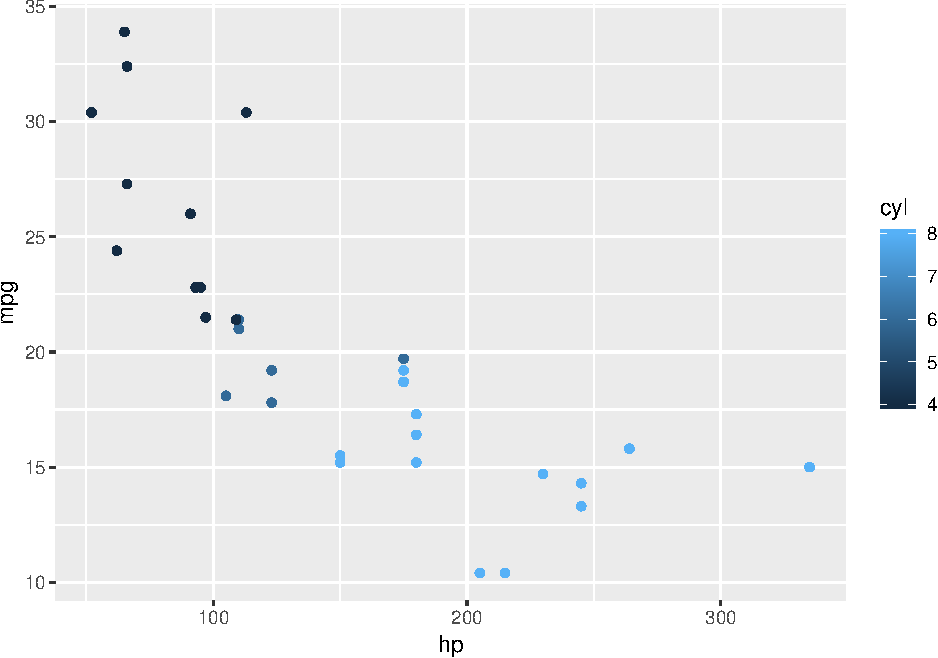
\includegraphics{_main_files/figure-latex/unnamed-chunk-22-1.pdf}

\begin{Shaded}
\begin{Highlighting}[]
\KeywordTok{ggplot}\NormalTok{(mtcars, }\KeywordTok{aes}\NormalTok{(hp, mpg, }\DataTypeTok{color =}\NormalTok{ cyl,}\DataTypeTok{label=}\KeywordTok{rownames}\NormalTok{(mtcars)))}\OperatorTok{+}
\StringTok{  }\KeywordTok{geom_text}\NormalTok{(}\DataTypeTok{size=}\DecValTok{3}\NormalTok{,}\DataTypeTok{check_overlap =} \OtherTok{TRUE}\NormalTok{)}
\end{Highlighting}
\end{Shaded}

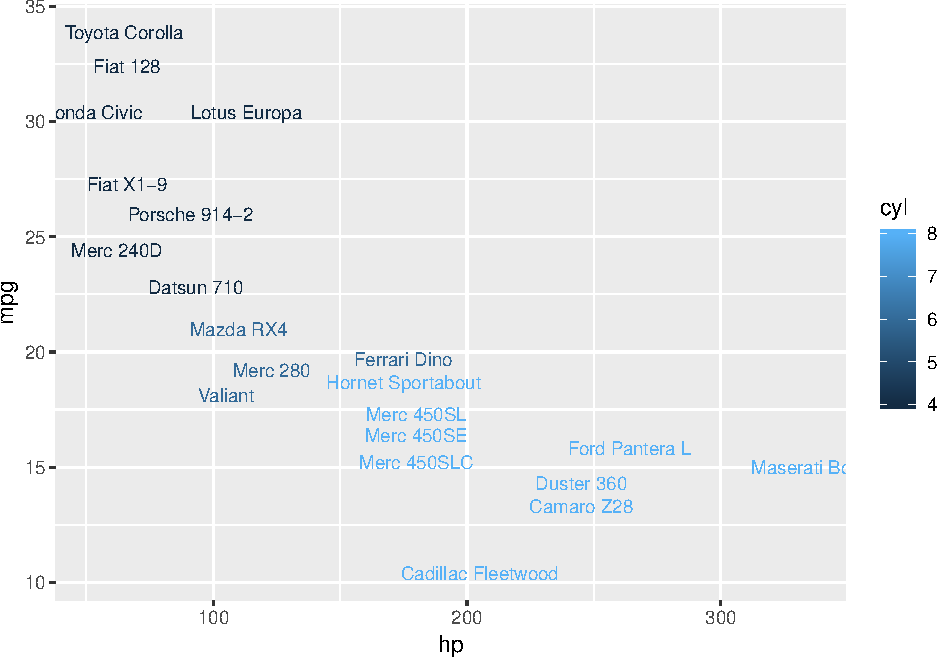
\includegraphics{_main_files/figure-latex/unnamed-chunk-22-2.pdf}

Vi kan benytte t til at transponere data matricen, så kan vi tegne et corrplot, det er meget mørkt da alle bilerne er positivt korrelerede, men man kan ane nogle sammenhænge. t(mtcars) betyder vi transponerer (vender) matricen, så ser vi i stedet på grupper af respondenter, som vi netop analyserer i klyngeanalysen. Hvis ikke vi vender matricen ser vi på korrelationsmatricen mellem de 11 variable i stedet, ligesom vi tidligere har gjort med faktoranalysen.

\begin{Shaded}
\begin{Highlighting}[]
\CommentTok{#korrelationsmatricen for transponeret mtcars data, hclust betyder vi ordner efter variable der passer sammen}
\NormalTok{pacman}\OperatorTok{::}\KeywordTok{p_load}\NormalTok{(corrplot)}
\KeywordTok{corrplot}\NormalTok{(}\KeywordTok{cor}\NormalTok{(}\KeywordTok{t}\NormalTok{(mtcars)), }\DataTypeTok{order =} \StringTok{"hclust"}\NormalTok{, }\DataTypeTok{tl.col=}\StringTok{'black'}\NormalTok{, }\DataTypeTok{tl.cex=}\NormalTok{.}\DecValTok{5}\NormalTok{)}
\end{Highlighting}
\end{Shaded}

\includegraphics{_main_files/figure-latex/unnamed-chunk-23-1.svg}

\begin{Shaded}
\begin{Highlighting}[]
\CommentTok{#Her er korrelationsmatricen ikke transponeret, hvilket svarer til en matrice baseret på variable som ved faktoranalysen vi tidligere så på.}
\KeywordTok{corrplot}\NormalTok{(}\KeywordTok{cor}\NormalTok{(mtcars), }\DataTypeTok{order =} \StringTok{"hclust"}\NormalTok{, }\DataTypeTok{tl.col=}\StringTok{'black'}\NormalTok{, }\DataTypeTok{tl.cex=}\NormalTok{.}\DecValTok{5}\NormalTok{)}
\end{Highlighting}
\end{Shaded}

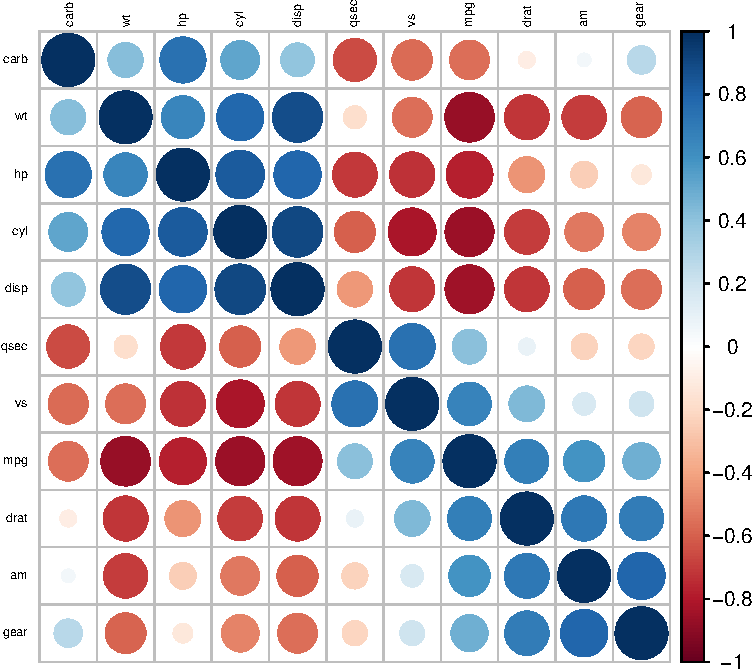
\includegraphics{_main_files/figure-latex/unnamed-chunk-24-1.pdf}

\hypertarget{hierakisk-klyngeanalyse-hclust-kommandoen}{%
\section{Hierakisk klyngeanalyse hclust kommandoen}\label{hierakisk-klyngeanalyse-hclust-kommandoen}}

Vi får nu R til at danne klynger vha. af hclust (hierarcical cluster) kommandoen, denne benytter default en metode der hedder complete til at finde ens klynger, der findes mange andre metoder. For at benytte hclust skal R først beregne afstandene mellem bilerne dette gøres med dist kommandoen. Algoritmen beregner afstandene mellem de forskellige bilmodeller vha. af den euklidiske metrik. Biler med kort afstand kommer i klynger sammen, biler med lang afstand kommer i forskellige klynger.

Nedenfor ses et udsnit af afstandende mellem hver af de 32 biler, det er en meget stor 32 \(\times\) 32 matrice, derfor har vi benyttet head for kun at vise noget af matricen. Fx er afstanden mellem to forskellige biler som en Mazda RX4 og en Lincoln Continental 318.05 hvilket er en stor afstand i forhold til fx. Mazda RX4 og Mazda RX4 Wag på kun 0.62. Bemærk hvordan supersportsvognen Maserati Bora har store afstande til de fleste af de øvrige biler, Maseratien var en komfortabel, rummeligere og kraftigere og tungere sportsvogn end fx. Ferrari Dino.

\begin{Shaded}
\begin{Highlighting}[]
\KeywordTok{head}\NormalTok{(}\KeywordTok{as.matrix}\NormalTok{(}\KeywordTok{dist}\NormalTok{(mtcars)))}
\end{Highlighting}
\end{Shaded}

\begin{verbatim}
##                     Mazda RX4 Mazda RX4 Wag Datsun 710 Hornet 4 Drive
## Mazda RX4           0.0000000     0.6153251   54.90861       98.11252
## Mazda RX4 Wag       0.6153251     0.0000000   54.89152       98.09589
## Datsun 710         54.9086059    54.8915169    0.00000      150.99352
## Hornet 4 Drive     98.1125212    98.0958939  150.99352        0.00000
## Hornet Sportabout 210.3374396   210.3358546  265.08316      121.02976
## Valiant            65.4717710    65.4392224  117.75470       33.55087
##                   Hornet Sportabout   Valiant Duster 360 Merc 240D
## Mazda RX4                  210.3374  65.47177  241.40765  50.15327
## Mazda RX4 Wag              210.3359  65.43922  241.40887  50.11461
## Datsun 710                 265.0832 117.75470  294.47902  49.65848
## Hornet 4 Drive             121.0298  33.55087  169.42996 121.27397
## Hornet Sportabout            0.0000 152.12414   70.17673 241.50697
## Valiant                    152.1241   0.00000  194.60945  89.59111
##                    Merc 230  Merc 280 Merc 280C Merc 450SE Merc 450SL
## Mazda RX4          25.46831  15.36419  15.67247  135.43070  135.40144
## Mazda RX4 Wag      25.32845  15.29569  15.58377  135.42548  135.39604
## Datsun 710         33.18038  66.93635  67.02614  189.19549  189.16317
## Hornet 4 Drive    118.24331  91.42240  91.46129   72.49643   72.43135
## Hornet Sportabout 233.49240 199.33450 199.34066   84.38885   84.36840
## Valiant            85.00796  60.29098  60.26557   90.69703   90.67697
##                   Merc 450SLC Cadillac Fleetwood Lincoln Continental
## Mazda RX4           135.47947           326.3396            318.0470
## Mazda RX4 Wag       135.47232           326.3355            318.0429
## Datsun 710          189.23454           381.0926            372.8012
## Hornet 4 Drive       72.57185           234.4404            227.9726
## Hornet Sportabout    84.43324           116.2804            108.0624
## Valiant              90.70930           266.6281            259.6304
##                   Chrysler Imperial  Fiat 128 Honda Civic Toyota Corolla
## Mazda RX4                 304.72034  93.26800   102.83076       100.6040
## Mazda RX4 Wag             304.71692  93.25310   102.82387       100.5888
## Datsun 710                359.30149  40.99338    52.77046        47.6535
## Hornet 4 Drive            218.15483 184.96897   191.55187       192.6714
## Hornet Sportabout          97.20491 302.03772   310.03246       309.5582
## Valiant                   248.77133 152.11533   158.96158       159.8303
##                   Toyota Corona Dodge Challenger AMC Javelin Camaro Z28
## Mazda RX4              42.30752        163.11508   149.60472  233.22288
## Mazda RX4 Wag          42.26592        163.11342   149.60145  233.22487
## Datsun 710             12.96547        217.77958   204.31889  286.00492
## Hornet 4 Drive        138.53047         72.44039    61.36019  163.66326
## Hornet Sportabout     252.33320         48.98389    61.42742   70.96653
## Valiant               105.28764        103.43107    91.04443  187.84638
##                   Pontiac Firebird Fiat X1-9 Porsche 914-2 Lotus Europa
## Mazda RX4                248.67803  92.50484      44.40337     65.73284
## Mazda RX4 Wag            248.67620  92.49400      44.40736     65.73626
## Datsun 710               303.35839  39.88151      13.13571     25.09486
## Hornet 4 Drive           156.22403 184.44712     139.15795    163.23674
## Hornet Sportabout         40.00525 301.56695     254.14526    272.35824
## Valiant                  188.52721 151.43794     106.05858    130.82482
##                   Ford Pantera L Ferrari Dino Maserati Bora Volvo 142E
## Mazda RX4               245.4247     66.76610      265.6454   39.18940
## Mazda RX4 Wag           245.4294     66.77642      265.6491   39.16260
## Datsun 710              297.2940     90.24155      309.7718   20.69394
## Hornet 4 Drive          180.1140    130.55230      229.3419  137.03633
## Hornet Sportabout        89.5934    215.06739      170.7094  248.00634
## Valiant                 203.0178    106.56948      242.4393  104.18637
\end{verbatim}

Vi gemmer hclust data i clusters variablen, vi så kan benytte til at tegne en oversigt over klyngerne.
Vi kan nu plotte en grafisk oversigt over bilerne. I nederste linje er den fineste inddeling, hvor samtlige biler er i deres egen klynge. Den blå linje med 3 skæringer i dendogrammet indikerer der er 3 klynger, den røde 4 klynger.

\begin{Shaded}
\begin{Highlighting}[]
\NormalTok{clusters <-}\StringTok{ }\KeywordTok{hclust}\NormalTok{(}\KeywordTok{dist}\NormalTok{(mtcars))}
\KeywordTok{plot}\NormalTok{(clusters,}\DataTypeTok{cex=}\FloatTok{0.5}\NormalTok{,}\DataTypeTok{main =} \StringTok{"Dendogram af mtcars"}\NormalTok{,}\DataTypeTok{xlab =} \StringTok{"Klyngetræ"}\NormalTok{,}\DataTypeTok{sub=}\StringTok{"Bilmodeller"}\NormalTok{)}
\KeywordTok{abline}\NormalTok{(}\DataTypeTok{h =} \DecValTok{190}\NormalTok{, }\DataTypeTok{col=}\StringTok{"red"}\NormalTok{) }\CommentTok{#Tegn rød vandret linje h betyder horisontal}
\KeywordTok{abline}\NormalTok{(}\DataTypeTok{h =} \DecValTok{230}\NormalTok{, }\DataTypeTok{col=}\StringTok{"blue"}\NormalTok{)}
\end{Highlighting}
\end{Shaded}

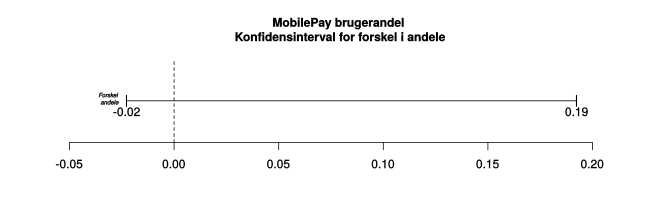
\includegraphics{_main_files/figure-latex/unnamed-chunk-26-1.svg}

Hvis vi ønsker at undersøge en indeling med et bestemt antal klynger, kan vi bruge cutree i R, til at undersøge klyngerne i en skæring med fx. 4 klynger nærmere. Her ser vi som nævnt, Maserati Bora skiller sig ud ved at have sin egen klynge. Nummeret ved hver af de 32 biler angiver hvilken klynge bilen tilhører.

\begin{Shaded}
\begin{Highlighting}[]
\NormalTok{clusterCut <-}\StringTok{ }\KeywordTok{cutree}\NormalTok{(clusters, }\DecValTok{4}\NormalTok{) }\CommentTok{#Opdeling i 4 klynger.}
\NormalTok{clusterCut}
\end{Highlighting}
\end{Shaded}

\begin{verbatim}
##           Mazda RX4       Mazda RX4 Wag          Datsun 710 
##                   1                   1                   1 
##      Hornet 4 Drive   Hornet Sportabout             Valiant 
##                   2                   3                   2 
##          Duster 360           Merc 240D            Merc 230 
##                   3                   1                   1 
##            Merc 280           Merc 280C          Merc 450SE 
##                   1                   1                   2 
##          Merc 450SL         Merc 450SLC  Cadillac Fleetwood 
##                   2                   2                   3 
## Lincoln Continental   Chrysler Imperial            Fiat 128 
##                   3                   3                   1 
##         Honda Civic      Toyota Corolla       Toyota Corona 
##                   1                   1                   1 
##    Dodge Challenger         AMC Javelin          Camaro Z28 
##                   2                   2                   3 
##    Pontiac Firebird           Fiat X1-9       Porsche 914-2 
##                   3                   1                   1 
##        Lotus Europa      Ford Pantera L        Ferrari Dino 
##                   1                   3                   1 
##       Maserati Bora          Volvo 142E 
##                   4                   1
\end{verbatim}

Vi kan benytte subset kommandoen til at se på hvilke variable der er i hver klynge, herunder ser vi på klynge 3.

\begin{Shaded}
\begin{Highlighting}[]
\KeywordTok{subset}\NormalTok{(clusterCut,clusterCut}\OperatorTok{==}\DecValTok{3}\NormalTok{)}
\end{Highlighting}
\end{Shaded}

\begin{verbatim}
##   Hornet Sportabout          Duster 360  Cadillac Fleetwood 
##                   3                   3                   3 
## Lincoln Continental   Chrysler Imperial          Camaro Z28 
##                   3                   3                   3 
##    Pontiac Firebird      Ford Pantera L 
##                   3                   3
\end{verbatim}

Vi kan ligeledes sammenligne klyngeinddelingen med de enkelte variable og se om disse passer sammen. Fx. passer hp meget fint med inddelingen i klynger.

\begin{Shaded}
\begin{Highlighting}[]
\KeywordTok{table}\NormalTok{(clusterCut, mtcars}\OperatorTok{$}\NormalTok{cyl)}
\end{Highlighting}
\end{Shaded}

\begin{verbatim}
##           
## clusterCut  4  6  8
##          1 11  5  0
##          2  0  2  5
##          3  0  0  8
##          4  0  0  1
\end{verbatim}

\begin{Shaded}
\begin{Highlighting}[]
\KeywordTok{table}\NormalTok{(clusterCut, mtcars}\OperatorTok{$}\NormalTok{mpg)}
\end{Highlighting}
\end{Shaded}

\begin{verbatim}
##           
## clusterCut 10.4 13.3 14.3 14.7 15 15.2 15.5 15.8 16.4 17.3 17.8 18.1 18.7
##          1    0    0    0    0  0    0    0    0    0    0    1    0    0
##          2    0    0    0    0  0    2    1    0    1    1    0    1    0
##          3    2    1    1    1  0    0    0    1    0    0    0    0    1
##          4    0    0    0    0  1    0    0    0    0    0    0    0    0
##           
## clusterCut 19.2 19.7 21 21.4 21.5 22.8 24.4 26 27.3 30.4 32.4 33.9
##          1    1    1  2    1    1    2    1  1    1    2    1    1
##          2    0    0  0    1    0    0    0  0    0    0    0    0
##          3    1    0  0    0    0    0    0  0    0    0    0    0
##          4    0    0  0    0    0    0    0  0    0    0    0    0
\end{verbatim}

\begin{Shaded}
\begin{Highlighting}[]
\KeywordTok{table}\NormalTok{(clusterCut, mtcars}\OperatorTok{$}\NormalTok{hp)}
\end{Highlighting}
\end{Shaded}

\begin{verbatim}
##           
## clusterCut 52 62 65 66 91 93 95 97 105 109 110 113 123 150 175 180 205 215
##          1  1  1  1  2  1  1  1  1   0   1   2   1   2   0   1   0   0   0
##          2  0  0  0  0  0  0  0  0   1   0   1   0   0   2   0   3   0   0
##          3  0  0  0  0  0  0  0  0   0   0   0   0   0   0   2   0   1   1
##          4  0  0  0  0  0  0  0  0   0   0   0   0   0   0   0   0   0   0
##           
## clusterCut 230 245 264 335
##          1   0   0   0   0
##          2   0   0   0   0
##          3   1   2   1   0
##          4   0   0   0   1
\end{verbatim}

\begin{Shaded}
\begin{Highlighting}[]
\KeywordTok{table}\NormalTok{(clusterCut, mtcars}\OperatorTok{$}\NormalTok{carb)}
\end{Highlighting}
\end{Shaded}

\begin{verbatim}
##           
## clusterCut 1 2 3 4 6 8
##          1 5 6 0 4 1 0
##          2 2 2 3 0 0 0
##          3 0 2 0 6 0 0
##          4 0 0 0 0 0 1
\end{verbatim}

\begin{Shaded}
\begin{Highlighting}[]
\KeywordTok{table}\NormalTok{(clusterCut, mtcars}\OperatorTok{$}\NormalTok{wt)}
\end{Highlighting}
\end{Shaded}

\begin{verbatim}
##           
## clusterCut 1.513 1.615 1.835 1.935 2.14 2.2 2.32 2.465 2.62 2.77 2.78
##          1     1     1     1     1    1   1    1     1    1    1    1
##          2     0     0     0     0    0   0    0     0    0    0    0
##          3     0     0     0     0    0   0    0     0    0    0    0
##          4     0     0     0     0    0   0    0     0    0    0    0
##           
## clusterCut 2.875 3.15 3.17 3.19 3.215 3.435 3.44 3.46 3.52 3.57 3.73 3.78
##          1     1    1    0    1     0     0    2    0    0    0    0    0
##          2     0    0    0    0     1     1    0    1    1    0    1    1
##          3     0    0    1    0     0     0    1    0    0    1    0    0
##          4     0    0    0    0     0     0    0    0    0    1    0    0
##           
## clusterCut 3.84 3.845 4.07 5.25 5.345 5.424
##          1    0     0    0    0     0     0
##          2    0     0    1    0     0     0
##          3    1     1    0    1     1     1
##          4    0     0    0    0     0     0
\end{verbatim}

Hvis dendogrammet virker lidt uoverskueligt, kan man vælge ape pakken for at lave mere fancy plots, her er rigtig mange muligheder.

\begin{Shaded}
\begin{Highlighting}[]
\CommentTok{#install.packages("ape")}
\KeywordTok{library}\NormalTok{(}\StringTok{"ape"}\NormalTok{)}
\NormalTok{colors =}\StringTok{ }\KeywordTok{c}\NormalTok{(}\StringTok{"red"}\NormalTok{, }\StringTok{"blue"}\NormalTok{, }\StringTok{"green"}\NormalTok{, }\StringTok{"pink"}\NormalTok{)}
\NormalTok{clus4 =}\StringTok{ }\KeywordTok{cutree}\NormalTok{(clusters, }\DecValTok{4}\NormalTok{)}
\KeywordTok{plot}\NormalTok{(}\KeywordTok{as.phylo}\NormalTok{(clusters), }\DataTypeTok{type =} \StringTok{"fan"}\NormalTok{, }\DataTypeTok{tip.color =}\NormalTok{ colors[clus4],}
     \DataTypeTok{label.offset =} \DecValTok{0}\NormalTok{, }\DataTypeTok{cex =} \FloatTok{0.5}\NormalTok{)}
\end{Highlighting}
\end{Shaded}

\includegraphics{_main_files/figure-latex/unnamed-chunk-30-1.svg}

Herunder er et plot, hvor farvekoden er baseret på klyngerne.

\begin{Shaded}
\begin{Highlighting}[]
\KeywordTok{ggplot}\NormalTok{(mtcars, }\KeywordTok{aes}\NormalTok{(hp, mpg)) }\OperatorTok{+}
\StringTok{  }\KeywordTok{geom_point}\NormalTok{(}\DataTypeTok{alpha =} \FloatTok{0.4}\NormalTok{, }\DataTypeTok{size =} \FloatTok{3.5}\NormalTok{) }\OperatorTok{+}\StringTok{ }\KeywordTok{geom_point}\NormalTok{(}\DataTypeTok{col =}\NormalTok{ clusterCut)}
\end{Highlighting}
\end{Shaded}

\includegraphics{_main_files/figure-latex/unnamed-chunk-31-1.svg}

\hypertarget{ikke-hierakisk-klyngeanalyse-kmeans-kommandoen}{%
\section{Ikke hierakisk klyngeanalyse kmeans kommandoen}\label{ikke-hierakisk-klyngeanalyse-kmeans-kommandoen}}

Vi kunne også have brugt kmeans metoden, her skal vi så angive hvor mange klynger, vi ønsker i analysen. Her benytter vi K-means og får 4 klynger med 7, 6, 9, 10 biler. I output fra R kan vi under Cluster means se gennemsnit, for de 4 klynger for alle 11 variable.

\begin{Shaded}
\begin{Highlighting}[]
\NormalTok{mtcarsCluster4 <-}\StringTok{ }\KeywordTok{kmeans}\NormalTok{(mtcars, }\DecValTok{4}\NormalTok{)}
\NormalTok{mtcarsCluster4}
\end{Highlighting}
\end{Shaded}

\begin{verbatim}
## K-means clustering with 4 clusters of sizes 10, 6, 7, 9
## 
## Cluster means:
##        mpg      cyl     disp       hp     drat       wt     qsec        vs
## 1 27.05000 4.000000 101.5700  81.4000 4.086000 2.199300 18.76100 0.9000000
## 2 16.83333 7.666667 284.5667 158.3333 3.033333 3.625000 17.76833 0.1666667
## 3 19.94286 5.714286 166.5714 120.1429 3.705714 3.107857 18.47143 0.5714286
## 4 14.64444 8.000000 388.2222 232.1111 3.343333 4.161556 16.40444 0.0000000
##          am     gear     carb
## 1 0.8000000 4.100000 1.500000
## 2 0.0000000 3.000000 2.333333
## 3 0.4285714 4.000000 3.571429
## 4 0.2222222 3.444444 4.000000
## 
## Clustering vector:
##           Mazda RX4       Mazda RX4 Wag          Datsun 710 
##                   3                   3                   1 
##      Hornet 4 Drive   Hornet Sportabout             Valiant 
##                   2                   4                   3 
##          Duster 360           Merc 240D            Merc 230 
##                   4                   1                   3 
##            Merc 280           Merc 280C          Merc 450SE 
##                   3                   3                   2 
##          Merc 450SL         Merc 450SLC  Cadillac Fleetwood 
##                   2                   2                   4 
## Lincoln Continental   Chrysler Imperial            Fiat 128 
##                   4                   4                   1 
##         Honda Civic      Toyota Corolla       Toyota Corona 
##                   1                   1                   1 
##    Dodge Challenger         AMC Javelin          Camaro Z28 
##                   2                   2                   4 
##    Pontiac Firebird           Fiat X1-9       Porsche 914-2 
##                   4                   1                   1 
##        Lotus Europa      Ford Pantera L        Ferrari Dino 
##                   1                   4                   3 
##       Maserati Bora          Volvo 142E 
##                   4                   1 
## 
## Within cluster sum of squares by cluster:
## [1] 10247.471  6355.581  8808.032 46659.317
##  (between_SS / total_SS =  88.4 %)
## 
## Available components:
## 
## [1] "cluster"      "centers"      "totss"        "withinss"    
## [5] "tot.withinss" "betweenss"    "size"         "iter"        
## [9] "ifault"
\end{verbatim}

Nedenfor ser vi på en tabel inddeling med 4 klynger med de 32 biler, sorteret efter antallet af cylindre.

\begin{Shaded}
\begin{Highlighting}[]
\KeywordTok{table}\NormalTok{(mtcarsCluster4}\OperatorTok{$}\NormalTok{cluster, mtcars}\OperatorTok{$}\NormalTok{cyl)}
\end{Highlighting}
\end{Shaded}

\begin{verbatim}
##    
##      4  6  8
##   1 10  0  0
##   2  0  1  5
##   3  1  6  0
##   4  0  0  9
\end{verbatim}

Nedenfor ser vi på en tabel inddeling med 3 klynger med de 32 biler, sorteret efter antallet af cylindre. Kører vi kmeans analysen igen, falder bilerne ikke nødvendigvis i samme klynger som tidligere, det skyldes algoritmen kan give forskellig optimale inddelinger.

\begin{Shaded}
\begin{Highlighting}[]
\NormalTok{mtcarsCluster3 <-}\StringTok{ }\KeywordTok{kmeans}\NormalTok{(mtcars, }\DecValTok{3}\NormalTok{)}
\KeywordTok{table}\NormalTok{(mtcarsCluster3}\OperatorTok{$}\NormalTok{cluster, mtcars}\OperatorTok{$}\NormalTok{cyl)}
\end{Highlighting}
\end{Shaded}

\begin{verbatim}
##    
##      4  6  8
##   1  0  7  0
##   2  0  0 14
##   3 11  0  0
\end{verbatim}

Vi kan lave et klyngeplot der viser forskellene på de 32 biler, herunder ses plottet med 3 klynger. Bemærk vi skal hente pakken \textbf{factoextra}, der indeholder plotfunktionen fviz\_cluster(). Vi har benyttet funktionen \textbf{scale()}, det er en rigtig god ide at benytte hvis, der er stor forskel på måleenhederne i en data.frame. Funktionen \textbf{scale()} bringer variablene i samme skale. Der er fx. stor forskel på enhederne i carb og disp, prøv at sammenligne nedenstående plot med et tilsvarende plot uden scale.

\begin{Shaded}
\begin{Highlighting}[]
\NormalTok{km3.res <-}\StringTok{ }\KeywordTok{kmeans}\NormalTok{(}\KeywordTok{scale}\NormalTok{(mtcars), }\DecValTok{3}\NormalTok{, }\DataTypeTok{nstart =} \DecValTok{25}\NormalTok{)}
\NormalTok{pacman}\OperatorTok{::}\KeywordTok{p_load}\NormalTok{(factoextra)}
\KeywordTok{fviz_cluster}\NormalTok{(km3.res, }\DataTypeTok{data =}\NormalTok{ mtcars, }\DataTypeTok{main =} \StringTok{"Klyngeplot biler opdelt i 3 klynger"}\NormalTok{,}\DataTypeTok{repel =} \OtherTok{TRUE}\NormalTok{)}
\end{Highlighting}
\end{Shaded}

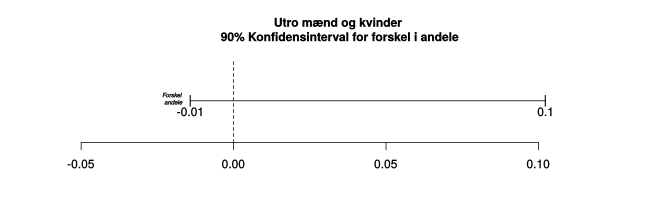
\includegraphics{_main_files/figure-latex/unnamed-chunk-35-1.svg}

Vi kan lave et klyngeplot der viser forskellene på de 32 biler, herunder ses plottet med 4 klynger.

\begin{Shaded}
\begin{Highlighting}[]
\NormalTok{km4.res <-}\StringTok{ }\KeywordTok{kmeans}\NormalTok{(}\KeywordTok{scale}\NormalTok{(mtcars), }\DecValTok{4}\NormalTok{, }\DataTypeTok{nstart =} \DecValTok{25}\NormalTok{)}
\KeywordTok{fviz_cluster}\NormalTok{(km4.res, }\DataTypeTok{data =}\NormalTok{ mtcars, }\DataTypeTok{main =} \StringTok{"Klyngeplot biler opdelt i 4 klynger"}\NormalTok{,}\DataTypeTok{repel =} \OtherTok{TRUE}\NormalTok{)}
\end{Highlighting}
\end{Shaded}

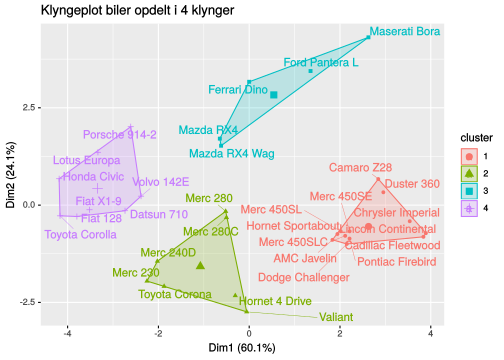
\includegraphics{_main_files/figure-latex/unnamed-chunk-36-1.svg}
Vi kan lave et klyngeplot der viser forskellene på de 32 biler, herunder ses plottet med 5 klynger.

\begin{Shaded}
\begin{Highlighting}[]
\NormalTok{km5.res <-}\StringTok{ }\KeywordTok{kmeans}\NormalTok{(}\KeywordTok{scale}\NormalTok{(mtcars), }\DecValTok{5}\NormalTok{, }\DataTypeTok{nstart =} \DecValTok{25}\NormalTok{)}
\KeywordTok{fviz_cluster}\NormalTok{(km5.res, }\DataTypeTok{data =}\NormalTok{ mtcars, }\DataTypeTok{main =} \StringTok{"Klyngeplot biler opdelt i 5 klynger"}\NormalTok{,}\DataTypeTok{repel =} \OtherTok{TRUE}\NormalTok{)}
\end{Highlighting}
\end{Shaded}

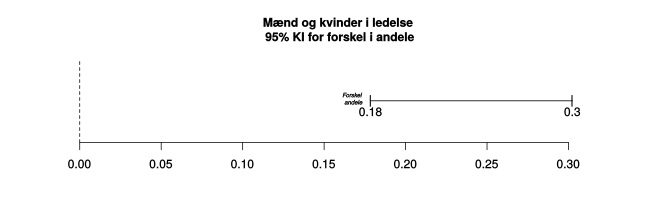
\includegraphics{_main_files/figure-latex/unnamed-chunk-37-1.svg}

\hypertarget{validering-med-anova}{%
\section{Validering med ANOVA}\label{validering-med-anova}}

Skal man undersøge om grupperne/klyngerne er forskellige med hensyn til de forskellige variable, kan man benytte Anova, hvor klyngerne er den uafhængige variabel. Man skal da gerne nå frem til at klyngegennemsnittede er signifikant forskellige mht. flere af variablene der indgår i analysen.

Spørgsmål US arrestationer samt urbaniseringsgrad

Lav en klyngeanalyse for datasæt med 50 observationer for amerikanske stater på 4 variable, data stammer fra World Almanac and Book of facts 1975. (Crime rates).

\begin{enumerate}
\def\labelenumi{\arabic{enumi}.}
\tightlist
\item
  Mord, antal arrestationer (pr 100,000)
\item
  Overfald, antal arrestationer (pr 100,000)
\item
  Urbaniseringsgrad andel af bybefolkning.
\item
  Voldtægt, antal arrestationer (pr 100,000)
\end{enumerate}

\begin{Shaded}
\begin{Highlighting}[]
\NormalTok{pacman}\OperatorTok{::}\KeywordTok{p_load}\NormalTok{(datasets)}
\NormalTok{arrest <-}\StringTok{ }\NormalTok{USArrests}
\KeywordTok{head}\NormalTok{(arrest)}
\end{Highlighting}
\end{Shaded}

\begin{verbatim}
##            Murder Assault UrbanPop Rape
## Alabama      13.2     236       58 21.2
## Alaska       10.0     263       48 44.5
## Arizona       8.1     294       80 31.0
## Arkansas      8.8     190       50 19.5
## California    9.0     276       91 40.6
## Colorado      7.9     204       78 38.7
\end{verbatim}

Undersøg om der kan dannes klynger og hvorledes disse kan karakteriseres. Illustrer grafisk og kommenter på karakteristika for klyngerne.

Svar US arrestationer samt urbaniseringsgrad kort version

Spørgsmål GDP

Download filen om GDP og GDP per capita her. Importer denne i R. Sørg for at få navnene for de enkelte lande som label, dette kan du fx. gøre ved nedenstående kommandoer:

Hvad betyder:
GDP{[}1:50,{]}
og
GDP{[},1{]}

\begin{Shaded}
\begin{Highlighting}[]
\NormalTok{GDP <-}\StringTok{ }\NormalTok{GDP[}\DecValTok{1}\OperatorTok{:}\DecValTok{50}\NormalTok{,]}
\KeywordTok{row.names}\NormalTok{(GDP) <-}\StringTok{ }\KeywordTok{as.matrix}\NormalTok{(GDP[,}\DecValTok{1}\NormalTok{])}

\KeywordTok{plot}\NormalTok{(clusters,}\DataTypeTok{cex=}\FloatTok{0.5}\NormalTok{,}\DataTypeTok{main =} \StringTok{"GDP"}\NormalTok{,}\DataTypeTok{xlab =} \StringTok{"Klyngetræ"}\NormalTok{,}\DataTypeTok{sub=}\StringTok{"GDP"}\NormalTok{)}
\end{Highlighting}
\end{Shaded}

Undersøg om der kan dannes klynger og hvorledes disse kan karakteriseres, der er rigtig mange observationer dvs. lande, se i stedet på deldatasæt der giver mening. Illustrer grafisk og kommenter på karakteristika for klyngerne.

Spørgsmål Forbes 100 US

Download filen om de 100 rigeste i USA her. Filen er tilrettet, dvs. binære kvalitative variable er kodet om til dummy variable.

Undersøg om der kan dannes klynger og hvorledes disse kan karakteriseres. Illustrer grafisk og kommenter på karakteristika for klyngerne.

Bemærk det er godt at sætte navnene på de velhavende som rækkenavne i din data.frame, for at det er nemmere at få et overblik i klyngetræ diagrammet, dette kan du fx. gøre som nedenfor:

\begin{Shaded}
\begin{Highlighting}[]
\KeywordTok{row.names}\NormalTok{(Forbes100) <-}\StringTok{ }\KeywordTok{as.matrix}\NormalTok{(Forbes100[,}\DecValTok{1}\NormalTok{])}
\NormalTok{clusters <-}\StringTok{ }\KeywordTok{hclust}\NormalTok{(}\KeywordTok{dist}\NormalTok{(Forbes100))}
\KeywordTok{plot}\NormalTok{(clusters,}\DataTypeTok{cex=}\FloatTok{0.5}\NormalTok{,}\DataTypeTok{main =} \StringTok{"US 100 Rigeste"}\NormalTok{,}\DataTypeTok{xlab =} \StringTok{"Klyngetræ"}\NormalTok{,}\DataTypeTok{sub=}\StringTok{"US top 100"}\NormalTok{)}
\end{Highlighting}
\end{Shaded}

Spørgsmål Valgfri datasæt
Find et valgfrit datasæt fx. på nettet, gennemfør en klyngeanalyse på dette datasæt.

\hypertarget{tidsrkker-og-arima}{%
\chapter{Tidsrækker og ARIMA}\label{tidsrkker-og-arima}}

\hypertarget{Sentry_noJS}{}
Sentry Page Protection

\hypertarget{Sentry_redirecting}{}
Please Wait\ldots{}

Gennemgangen af tidsrækkeanalyse bygger meget på praktisk anvendelighed (dvs. vi vil gerne kunne forudsige kursudviklingen), vi vil springe let hen over teorien der kan være tung og er meget omfattende. Nedenstående links giver dog en indføring i den teoretiske del, som vi her ikke berører.

\url{http://ucanalytics.com/blogs/arima-models-manufacturing-case-study-example-part-3/}

\url{http://ucanalytics.com/blogs/step-by-step-graphic-guide-to-forecasting-through-arima-modeling-in-r-manufacturing-case-study-example/}

Her er en gennemgang af forskellige typer af tidsrækker man kan opleve.

\url{https://people.duke.edu/~rnau/411arim.htm\#arima010}

Video om ARIMA
\url{https://youtu.be/Aw77aMLj9uM}

En tidsrække er observationer, der er observeret over tid, fx. lukkekursen på Novo i 2018, kan vi beskrive som en tidsrække. Hvor vi både registrerer dato og lukkekursen. ARIMA er et avanceret analyseværktøj til at beskrive tidsrækker. Vi vil i de følgende kaptiler, med eksempler beskrive hvordan de enkelte elementer i ARIMA rent praktisk fungerer.

\textbf{\emph{AR}} står for AutoRegressive
\textbf{\emph{I}} står for Integrated
\textbf{\emph{MA}} står for Moving Average

Lad i de følgende afsnit se på nogle simple eksempler for trinvis, at kunne beskrive hvorledes modellen fungerer.

\hypertarget{arima000}{%
\section{ARIMA(0,0,0)}\label{arima000}}

Nedenfor har vi aktiekurser for 50 dage for en fiktiv aktie, vi vil nu undersøge om disse kan bruges til at forudsige noget om fremtidige aktiekurser. For at gøre dette, skal man enten importere Excelfilen, eller copy paste data fra rammen nedenfor.

Hent ARIMA1.xlsx Excel filen her. Importer ARIMA1.xlsx til R via menuen File - Import Dataset - Excel. Nu skal datasættet rettes til en tidsserie med ts() kommandoen.

\begin{Shaded}
\begin{Highlighting}[]
\NormalTok{ARIMA1 <-}\StringTok{ }\KeywordTok{ts}\NormalTok{(ARIMA1)}
\end{Highlighting}
\end{Shaded}

Vi kan nu plotte vore data i R.

\begin{Shaded}
\begin{Highlighting}[]
\KeywordTok{plot.ts}\NormalTok{(ARIMA1, }\DataTypeTok{xlab=}\StringTok{'Tid'}\NormalTok{, }\DataTypeTok{ylab =} \StringTok{'Kursdata'}\NormalTok{)}
\end{Highlighting}
\end{Shaded}

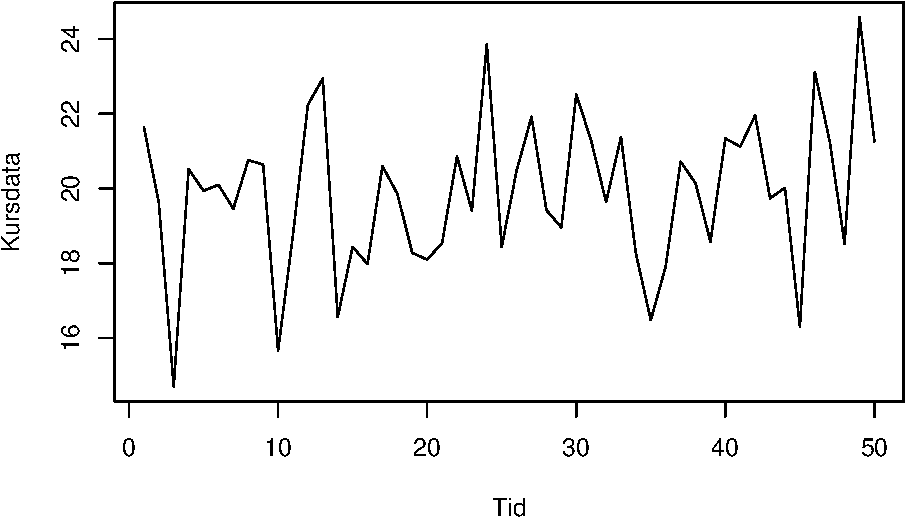
\includegraphics{_main_files/figure-latex/unnamed-chunk-43-1.pdf}

Det er svært at se nogen tydelig udvikling i kursen.

Vi benytter auto.arima til at undersøge om der er en systematik i tidsserien, for at bruge denne funktion skal vi hente og loade pakken forecast med fx. pacman:

Funktionen auto.arima i R er en fantastisk funktion, der automatisk finder den ARIMA model, der passer bedst på observationerne.

\begin{Shaded}
\begin{Highlighting}[]
\KeywordTok{auto.arima}\NormalTok{(ARIMA1)}
\end{Highlighting}
\end{Shaded}

\begin{verbatim}
## Series: ARIMA1 
## ARIMA(0,0,0) with non-zero mean 
## 
## Coefficients:
##          mean
##       19.8964
## s.e.   0.2872
## 
## sigma^2 estimated as 4.209:  log likelihood=-106.37
## AIC=216.74   AICc=217   BIC=220.57
\end{verbatim}

Output ARIMA(0,0,0) with non-zero mean, fortæller os at data er ligesom hvid støj. Den bedste forudsigelse af aktieprisen, vi kan komme med er gennemsnittet af alle kurserne. Vi kan altså ikke forudsige prisen vha. vore fine værktøjer.

Akaike Information Criterion (AIC) , og Bayesian Information Criterion (BIC) benyttes til at vælge ARIMA modellen med mindst AIC og BIC værdier. auto.arima finder den bedste model automatisk.

Her er ligningen for aktiekursen, den bedste forudsigelse af den fremtidige kurs er den gennemsnitlige kurs der tidligere er observeret.

\[\hat{Y_t}=19.90\]

Variablen \(\hat{Y}_t\), kaldet Y hat t angiver vort estimat (gæt) på aktiekursen på tidspunkt \(t=1,2,3,...\). Der er således så lidt systematik i Data at her er tale om en ARIMA(0,0,0) model. Vi ser også at der står ``ARIMA(0,0,0) with non-zero mean'' i output fra R.

\hypertarget{arima100-eller-ar1-autoregression}{%
\section{ARIMA(1,0,0) eller AR(1) autoregression}\label{arima100-eller-ar1-autoregression}}

En ARIMA(1,0,0) model kan skrives som:

\[\hat{Y_t}=c + \phi Y_{t-1}\]

Vi kan forklare \(\hat{Y_t}\) er værdien for tidsrækken på tidspunkt \(t\), ud fra en konstant \(c\) plus en faktor \(\phi\), der ganges på værdien for tidsrækken på tidspunkt \(t-1\). For at bestemme c skal vi kende tidsrækkens sande middelværdi \(\mu\) og \(\phi\), disse værdier kan R beregne for os. Vi kan så beregne konstanten \(c=(1-\phi)\cdot \mu\). Det betyder så at vi kan estimere fremtidige værdier tidsrækken.

Vi har nu et eksempel hvor den sande middelværdi for tidsrækken er \(\mu=100\) og \(\phi=0.5\) for en ARIMA(1,0,0) model. Så kan vi beregne \(c=(1-\phi)\cdot \mu=(1-0.5)\cdot 100=50\) er middelværdien estimeret ved den gennemsnitlige kurs. Ligningen for modellen kan så skrives som:

\[\hat{Y_t}=c + \phi Y_{t-1} \Leftrightarrow \hat{Y_t}=50 + 0.5 Y_{t-1}\]

\(\phi\) fortæller, hvis kursen dagen før var 80 gennemsnitskursen er 100, vil kursen imorgen \(t=1\) ifølge modellen være forudsagt som:
\[50+0.5\cdot 80=90\]
Dagen efter \(t=2\) vil kursen så være forudsagt til:
\[50+0.5\cdot 90=95\]
Om 3 dage dvs. \(t=3\) vil kursen så være forudsagt til:
\[50+0.5\cdot 95=97.5\]
Om 4 dage dvs. \(t=4\) vil kursen så være forudsagt til:
\[50+0.5\cdot 97.5=98.75\]

Osv..

Vi siger at forudsagte værdier konvergerer mod (dvs. nærmer sig) \(\mu=100\).

AR i ARIMA, står for autoregression, selv-regression mod middelværdien, i eksemplet så vi hvordan værdien nærmer sig 100, hvis vi forudsiger flere dages kurser kan vi se dette.

\(\phi\) må kun antage værdier mellem og ikke lig med -1 og 1, hvilket betyder den er stationær, altså nærmer sig den sande middelværdi \(\mu\).

Hvad vil der ske hvis \(\mu=100\) og \(\phi=-0.5\) for en ARIMA(1,0,0) model (husk \(c=(1-\phi)\cdot\mu\) når man skal bestemme modellen)?

Hent ARIMA2.xlsx Excel filen her. Importer ARIMA2.xlsx til R via menuen File - Import Dataset - Excel. Nu skal datasættet rettes til en tidsserie med ts() kommandoen.

\begin{Shaded}
\begin{Highlighting}[]
\NormalTok{ARIMA2 <-}\StringTok{ }\KeywordTok{ts}\NormalTok{(ARIMA2)}
\end{Highlighting}
\end{Shaded}

\begin{Shaded}
\begin{Highlighting}[]
\NormalTok{aaa2 <-}\StringTok{ }\KeywordTok{auto.arima}\NormalTok{(ARIMA2)}
\NormalTok{aaa2}
\end{Highlighting}
\end{Shaded}

\begin{verbatim}
## Series: ARIMA2 
## ARIMA(1,0,0) with non-zero mean 
## 
## Coefficients:
##          ar1      mean
##       0.3664  103.2372
## s.e.  0.1301    2.4492
## 
## sigma^2 estimated as 128.3:  log likelihood=-191.36
## AIC=388.73   AICc=389.25   BIC=394.46
\end{verbatim}

Her afslører auto.arima 1. ordens autoregression dvs.

Modellen kan skrives som.

\[\hat{Y_t}=c + \phi Y_{t-1}\Leftrightarrow \hat{Y_t}=(1-0.3664)\cdot 103.2372 + 0.3664Y_{t-1}\Leftrightarrow \hat{Y_t}=65.4125 + 0.3664Y_{t-1}\]

Vi ser nu igen på vores eksempel med ARIMA2, vi kan nu i R forudsige aktiekursen 12 perioder frem med predict:

\begin{Shaded}
\begin{Highlighting}[]
\KeywordTok{predict}\NormalTok{(}\KeywordTok{auto.arima}\NormalTok{(ARIMA2), }\DataTypeTok{n.ahead =} \DecValTok{12}\NormalTok{)}\OperatorTok{$}\NormalTok{pred}
\end{Highlighting}
\end{Shaded}

\begin{verbatim}
## Time Series:
## Start = 51 
## End = 62 
## Frequency = 1 
##  [1] 105.3673 104.0177 103.5232 103.3420 103.2756 103.2513 103.2424
##  [8] 103.2391 103.2379 103.2375 103.2373 103.2373
\end{verbatim}

Spørgsmål ARIMA(1,0,0)
Hent ARIMA22.xlsx Excel filen her. Importer ARIMA22.xlsx til R via menuen File - Import Dataset - Excel. Bestem for den fremtidige aktiekurs 15 perioder frem, udregn direkte fx. vha. Excel og tjek dit resultat i R.

Svar ARIMA(1,0,0)

\begin{Shaded}
\begin{Highlighting}[]
\NormalTok{ARIMA22 <-}\StringTok{ }\KeywordTok{ts}\NormalTok{(ARIMA22)}
\NormalTok{aaa22 <-}\StringTok{ }\KeywordTok{auto.arima}\NormalTok{(ARIMA22)}
\NormalTok{aaa22}
\end{Highlighting}
\end{Shaded}

\begin{verbatim}
## Series: ARIMA22 
## ARIMA(1,0,0) with non-zero mean 
## 
## Coefficients:
##          ar1      mean
##       0.2286  215.4871
## s.e.  0.1371    2.3978
## 
## sigma^2 estimated as 180.3:  log likelihood=-199.82
## AIC=405.63   AICc=406.15   BIC=411.37
\end{verbatim}

\begin{Shaded}
\begin{Highlighting}[]
\KeywordTok{predict}\NormalTok{(}\KeywordTok{auto.arima}\NormalTok{(ARIMA22), }\DataTypeTok{n.ahead =} \DecValTok{15}\NormalTok{)}\OperatorTok{$}\NormalTok{pred}
\end{Highlighting}
\end{Shaded}

\begin{verbatim}
## Time Series:
## Start = 51 
## End = 65 
## Frequency = 1 
##  [1] 216.7592 215.7779 215.5536 215.5023 215.4905 215.4878 215.4872
##  [8] 215.4871 215.4871 215.4871 215.4871 215.4871 215.4871 215.4871
## [15] 215.4871
\end{verbatim}

Spørgsmål ARIMA(1,0,0)
Hent ARIMA23.xlsx Excel filen her. Importer ARIMA23.xlsx til R via menuen File - Import Dataset - Excel. Bestem for den fremtidige aktiekurs 15 perioder frem, udregn direkte fx. vha. Excel og tjek dit resultat i R.

\hypertarget{arima010-eller-i1-random-walk-with-a-drift}{%
\section{ARIMA(0,1,0) eller I(1) Random Walk with a drift}\label{arima010-eller-i1-random-walk-with-a-drift}}

Hvis en serie er ikke-stationær, er den simpleste model en random walk:

\[\hat{Y_t}-Y_{t-1}=\mu\Leftrightarrow \hat{Y_t}=Y_{t-1}+\mu\]
Dette betyder at Y stiger konstant med \(\mu\) i hver periode. Drift betyder at tidsrækken stiger konstant.

Forestiller man sig en ARIMA(0,1,0) med drift 10 og en kurs på tidspunkt t-1 på 120, vil vi forudsige en kurs på 130 ved tid t og 140 ved tid t+1 osv. Vi kan opskrive modellen som:
\[\hat{Y_t}-Y_{t-1}=10\Leftrightarrow \hat{Y_t}=Y_{t-1}+10\]

Hent ARIMA3.xlsx Excel filen her. Importer ARIMA3.xlsx til R via menuen File - Import Dataset - Excel. Nu skal datasættet rettes til en tidsserie med ts() kommandoen.

\begin{Shaded}
\begin{Highlighting}[]
\KeywordTok{ts.plot}\NormalTok{(ARIMA3)}
\end{Highlighting}
\end{Shaded}

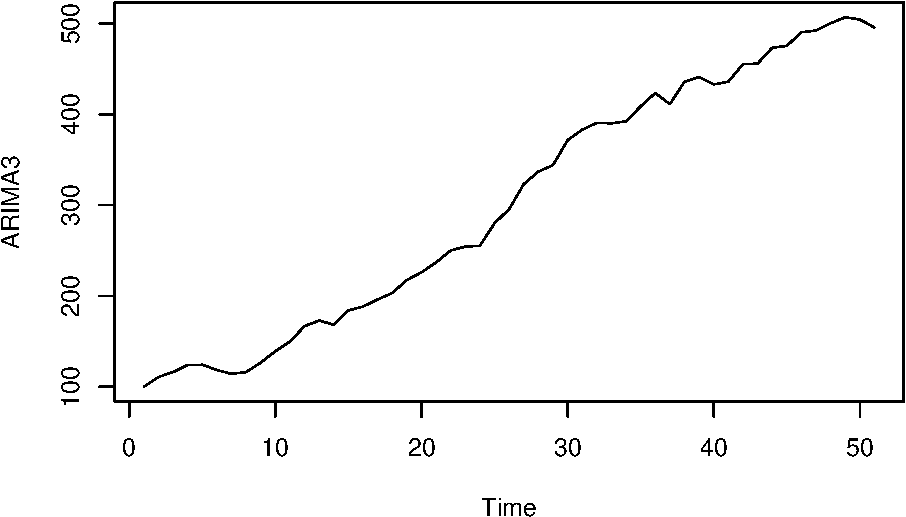
\includegraphics{_main_files/figure-latex/unnamed-chunk-54-1.pdf}

\begin{Shaded}
\begin{Highlighting}[]
\KeywordTok{auto.arima}\NormalTok{(ARIMA3)}
\end{Highlighting}
\end{Shaded}

\begin{verbatim}
## Series: ARIMA3 
## ARIMA(0,1,0) with drift 
## 
## Coefficients:
##        drift
##       7.9149
## s.e.  1.2790
## 
## sigma^2 estimated as 83.46:  log likelihood=-181.05
## AIC=366.1   AICc=366.36   BIC=369.93
\end{verbatim}

Modellen ovenfor kan skrives som:
\[\hat{Y_t}-Y_{t-1}=\mu\Leftrightarrow \hat{Y_t}-Y_{t-1}=7.9\Leftrightarrow \hat{Y_t}=Y_{t-1}+7.9\]
Vi indsætter drift i stedet for \(\mu\), tolningen er at modellen forudsiger at aktiekursen stiger med 7.9 fra periode til periode.

Hvis vi har en ren random walk model uden drift dvs. med \(\mu=0\) ARIMA(0,1,0) for en aktiekurs , forventer vi at kursen til tid t vil være den samme som til tid t-1. Denne kan skrives som:

\[\hat{Y_t}-Y_{t-1}=0\]

\hypertarget{arima001-eller-ma1-moving-average}{%
\section{ARIMA(0,0,1) eller MA(1) Moving average}\label{arima001-eller-ma1-moving-average}}

Vi kan i stedet for at bruge tidligere aktiekurser til at forudsige aktiekursen i stedet benytte tidligere målefejl residualer til at forudsige kursen.

Modellen kan skrives som:

\[\hat{Y_t}=\mu+\theta_1 e_{t-1}\]
Hvis vi forestiller os \(\mu=50\) \(\theta_1=0.5\) kursen til tid t-1 var 120 forudsigelsen til tid t-1 var 100, så målefejlen residualen til tid t-1 er \(e_{t-1}\) er faktisk kurs minus forudsagt kurs altså 120-100=20. Nu kan vi forudsige kursen til tid t som:
\[\hat{Y_t}=\mu+\theta_1 e_{t-1}\Leftrightarrow \hat{Y_t}=50+0.5\cdot20=60\]

Hent ARIMA4.xlsx Excel filen her. Importer ARIMA4.xlsx til R via menuen File - Import Dataset - Excel. Nu skal datasættet rettes til en tidsserie med ts() kommandoen.

\begin{Shaded}
\begin{Highlighting}[]
\KeywordTok{ts.plot}\NormalTok{(ARIMA4)}
\end{Highlighting}
\end{Shaded}

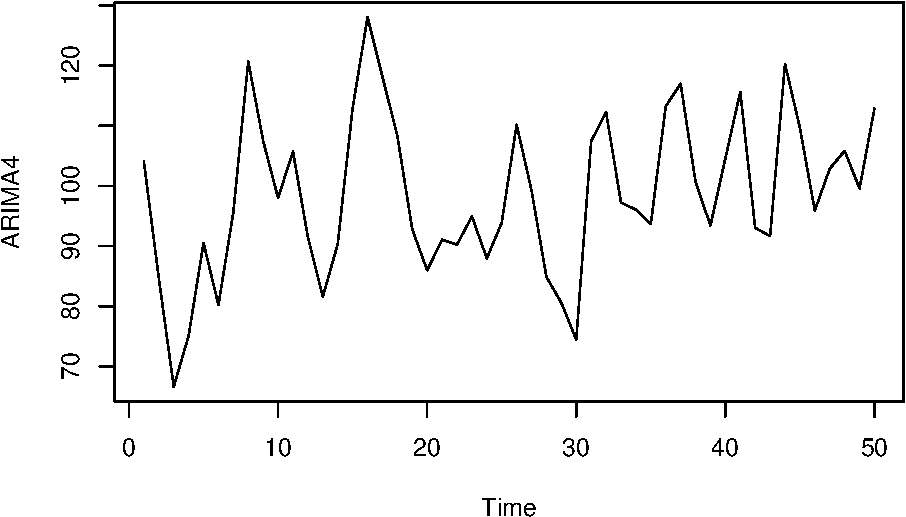
\includegraphics{_main_files/figure-latex/unnamed-chunk-56-1.pdf}

\begin{Shaded}
\begin{Highlighting}[]
\KeywordTok{auto.arima}\NormalTok{(ARIMA4)}
\end{Highlighting}
\end{Shaded}

\begin{verbatim}
## Series: ARIMA4 
## ARIMA(0,0,1) with non-zero mean 
## 
## Coefficients:
##          ma1     mean
##       0.9053  99.0176
## s.e.  0.0664   2.5588
## 
## sigma^2 estimated as 95.68:  log likelihood=-184.81
## AIC=375.62   AICc=376.14   BIC=381.35
\end{verbatim}

Vi kan nu forudsige aktiekursen 12 perioder frem med predict:

\begin{Shaded}
\begin{Highlighting}[]
\KeywordTok{predict}\NormalTok{(}\KeywordTok{auto.arima}\NormalTok{(ARIMA4), }\DataTypeTok{n.ahead =} \DecValTok{12}\NormalTok{)}\OperatorTok{$}\NormalTok{pred}
\end{Highlighting}
\end{Shaded}

\begin{verbatim}
## Time Series:
## Start = 51 
## End = 62 
## Frequency = 1 
##  [1] 113.64960  99.01756  99.01756  99.01756  99.01756  99.01756  99.01756
##  [8]  99.01756  99.01756  99.01756  99.01756  99.01756
\end{verbatim}

Hvorfor svarer den forudsagte værdi til mean i en ren ARIMA(0,0,1) eller MA(1) model? (Vink hvad er definitionen på en residual)

\hypertarget{plots-med-forskellige-modeller}{%
\section{Plots med forskellige modeller}\label{plots-med-forskellige-modeller}}

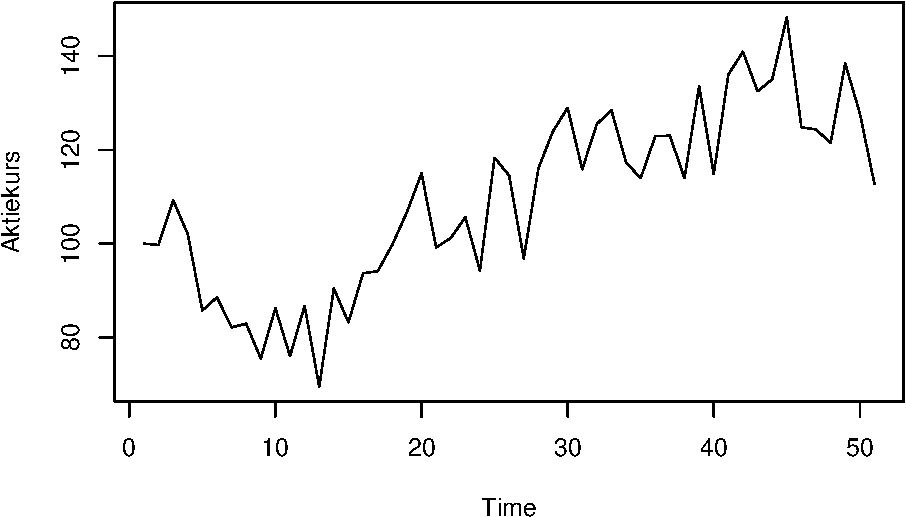
\includegraphics{_main_files/figure-latex/unnamed-chunk-58-1.pdf}

\begin{verbatim}
## Series: ap1 
## ARIMA(0,1,1) 
## 
## Coefficients:
##           ma1
##       -0.5239
## s.e.   0.1078
## 
## sigma^2 estimated as 105.2:  log likelihood=-187.01
## AIC=378.02   AICc=378.27   BIC=381.84
\end{verbatim}

Kursen svinger omkring middelværdien.

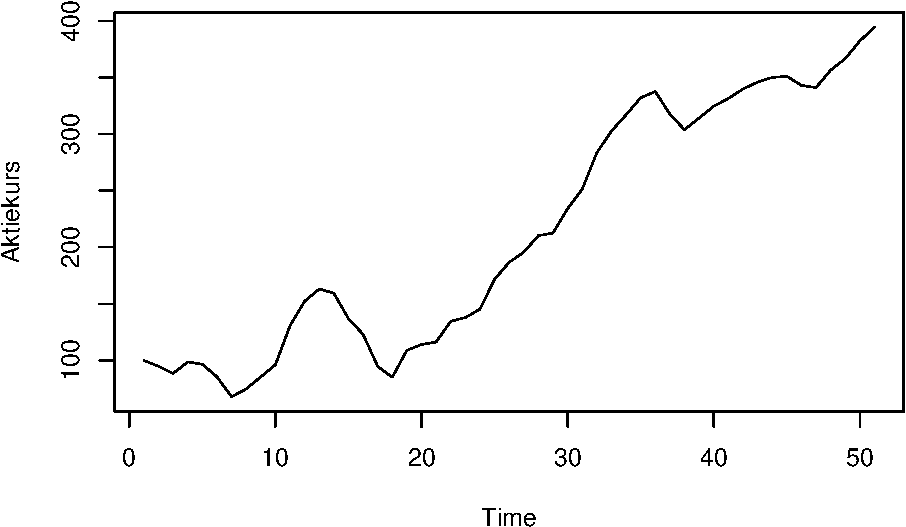
\includegraphics{_main_files/figure-latex/unnamed-chunk-59-1.pdf}

\begin{verbatim}
## Series: ap2 
## ARIMA(0,1,1) with drift 
## 
## Coefficients:
##          ma1   drift
##       0.5923  5.8685
## s.e.  0.1159  2.5505
## 
## sigma^2 estimated as 135.6:  log likelihood=-192.89
## AIC=391.77   AICc=392.3   BIC=397.51
\end{verbatim}

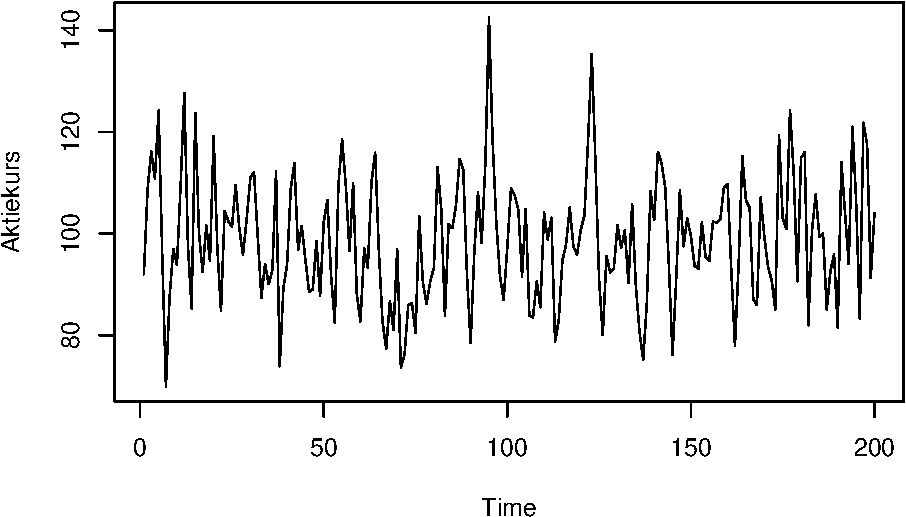
\includegraphics{_main_files/figure-latex/unnamed-chunk-60-1.pdf}

\begin{verbatim}
## Series: ap3 
## ARIMA(0,0,2) with non-zero mean 
## 
## Coefficients:
##          ma1      ma2     mean
##       0.4496  -0.1509  98.8406
## s.e.  0.0684   0.0679   1.0279
## 
## sigma^2 estimated as 127.4:  log likelihood=-767.16
## AIC=1542.32   AICc=1542.53   BIC=1555.51
\end{verbatim}

Vi kan også grafisk vise hvordan kursen vil udvikle sig med 80\% og 95\% konfidensbælter.

\begin{Shaded}
\begin{Highlighting}[]
\KeywordTok{forecast}\NormalTok{(}\KeywordTok{auto.arima}\NormalTok{(ap3))}
\end{Highlighting}
\end{Shaded}

\begin{verbatim}
##     Point Forecast    Lo 80    Hi 80    Lo 95    Hi 95
## 201      103.26827 88.80584 117.7307 81.14990 125.3867
## 202       97.61752 81.76051 113.4745 73.36631 121.8687
## 203       98.84056 82.83401 114.8471 74.36065 123.3205
## 204       98.84056 82.83401 114.8471 74.36065 123.3205
## 205       98.84056 82.83401 114.8471 74.36065 123.3205
## 206       98.84056 82.83401 114.8471 74.36065 123.3205
## 207       98.84056 82.83401 114.8471 74.36065 123.3205
## 208       98.84056 82.83401 114.8471 74.36065 123.3205
## 209       98.84056 82.83401 114.8471 74.36065 123.3205
## 210       98.84056 82.83401 114.8471 74.36065 123.3205
\end{verbatim}

\begin{Shaded}
\begin{Highlighting}[]
\KeywordTok{plot}\NormalTok{(}\KeywordTok{forecast}\NormalTok{(}\KeywordTok{auto.arima}\NormalTok{(ap3)))}
\end{Highlighting}
\end{Shaded}

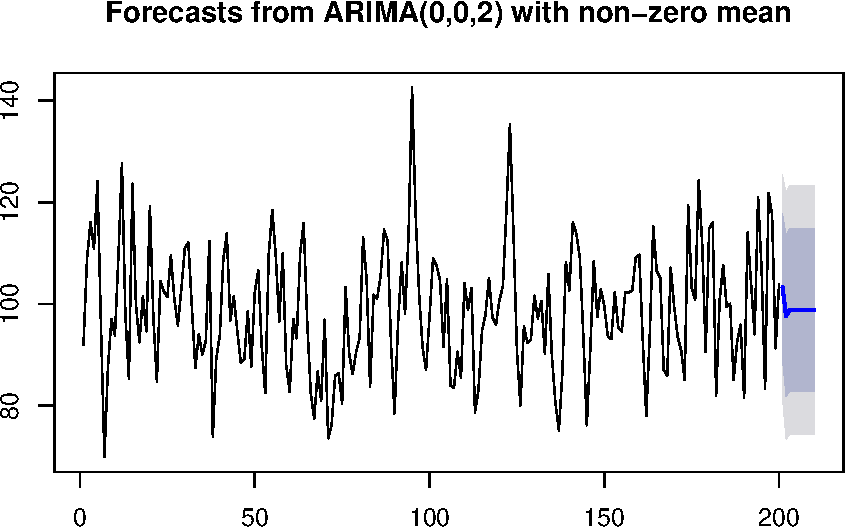
\includegraphics{_main_files/figure-latex/unnamed-chunk-61-1.pdf}

\hypertarget{arima-af-hjere-orden}{%
\section{ARIMA af højere orden}\label{arima-af-hjere-orden}}

Arima modeller kan afhænge af flere tidligere perioder, fx kan ligningen for ARIMA(2,0,0) eller AR(2), opskrives som:

\[\hat{Y_t}=c + \phi Y_{t-1}+ \phi_2 Y_{t-2}\]
Modellen afhænger altså af 2 tidligere perioder (lags) og ikke en. Man betegner dette som en model med lag 2.

Arima modeller kan indeholde flere forskellige elementer med lag som fx. ARIMA(0,2,1).

\hypertarget{arima-og-ssonalitet}{%
\section{ARIMA og sæsonalitet}\label{arima-og-ssonalitet}}

Hvis fx. en aktie handles lavere om fredagen kan ARIMA modellerne korrigere for dette ved sæsonkorrektion. I sæsonkorrigerede modeller vises dette som en ekstra vektor med 3 tal for hhv. sæsonkorrigeret AR eller SAR, sæsonkorrigeret I eller SI og sæsonkorrigeret MA eller SMA. En model som ARIMA(1,0,0)(1,0,0) har altså udover AR også en sæsonkomponent.

\hypertarget{arima-eksempler}{%
\section{ARIMA eksempler}\label{arima-eksempler}}

\hypertarget{traktorer}{%
\subsection{Traktorer}\label{traktorer}}

Hent følgende data for traktor salg, med følgende kommandoer i R.

\begin{Shaded}
\begin{Highlighting}[]
\NormalTok{data =}\StringTok{ }\KeywordTok{read.csv}\NormalTok{(}\StringTok{'http://ucanalytics.com/blogs/wp-content/uploads/2015/06/Tractor-Sales.csv'}\NormalTok{)}
\NormalTok{data =}\StringTok{ }\KeywordTok{ts}\NormalTok{(data[,}\DecValTok{2}\NormalTok{],}\DataTypeTok{start =} \KeywordTok{c}\NormalTok{(}\DecValTok{2003}\NormalTok{,}\DecValTok{1}\NormalTok{),}\DataTypeTok{frequency =} \DecValTok{12}\NormalTok{)}
\end{Highlighting}
\end{Shaded}

Vi ser salget er voksende over tid, der er ligeledes en sæsonkomponent.

\begin{Shaded}
\begin{Highlighting}[]
\KeywordTok{plot}\NormalTok{(data, }\DataTypeTok{xlab=}\StringTok{'Years'}\NormalTok{, }\DataTypeTok{ylab =} \StringTok{'Tractor Sales'}\NormalTok{)}
\end{Highlighting}
\end{Shaded}

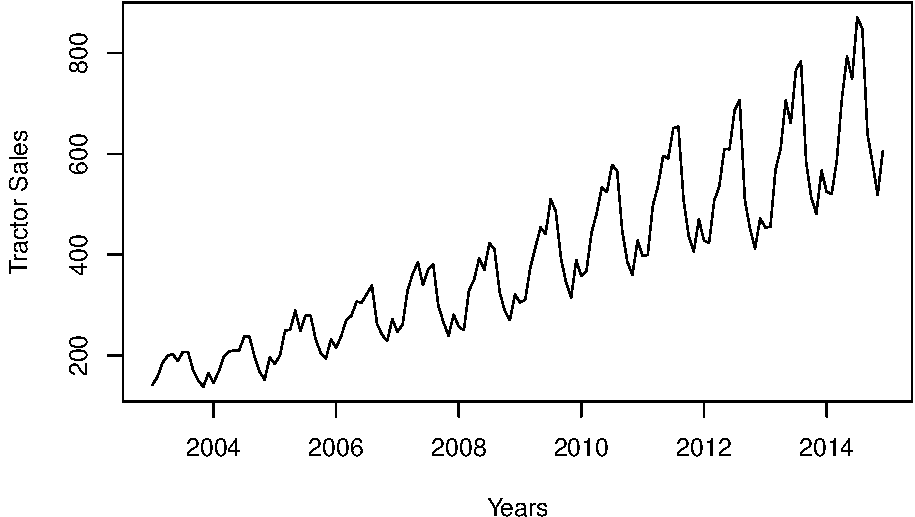
\includegraphics{_main_files/figure-latex/unnamed-chunk-63-1.pdf}

Differens tranformer data for at generere stationære data mht. middel (fjern trend)

\begin{Shaded}
\begin{Highlighting}[]
\KeywordTok{plot}\NormalTok{(}\KeywordTok{diff}\NormalTok{(data),}\DataTypeTok{ylab=}\StringTok{'Differenced Tractor Sales'}\NormalTok{)}
\end{Highlighting}
\end{Shaded}

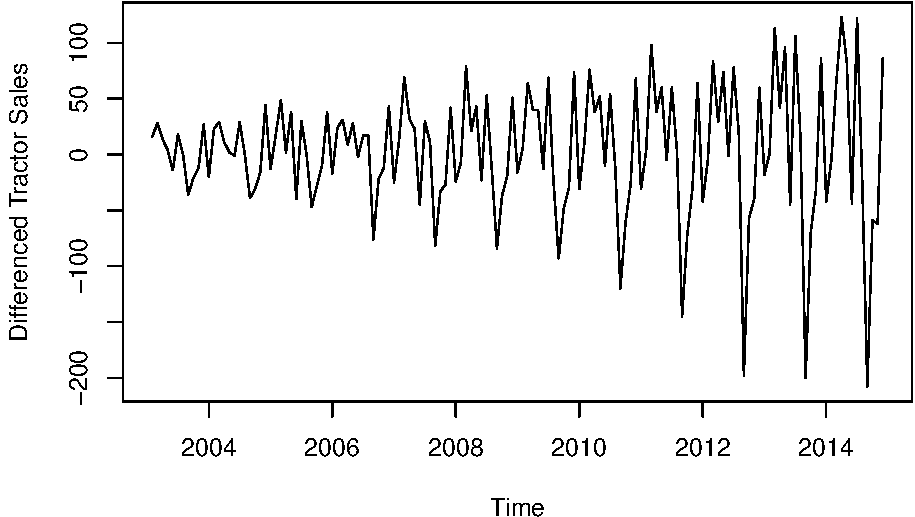
\includegraphics{_main_files/figure-latex/unnamed-chunk-64-1.pdf}

log transformer data for at sikre stationaritet mht. varians.

\begin{Shaded}
\begin{Highlighting}[]
\KeywordTok{plot}\NormalTok{(}\KeywordTok{log10}\NormalTok{(data),}\DataTypeTok{ylab=}\StringTok{'Log (Tractor Sales)'}\NormalTok{)}
\end{Highlighting}
\end{Shaded}

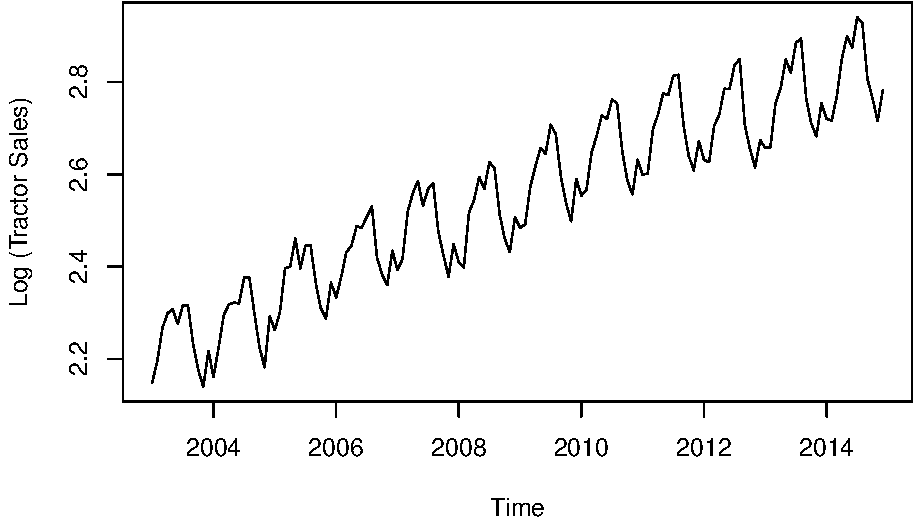
\includegraphics{_main_files/figure-latex/unnamed-chunk-65-1.pdf}

Eventuel Differens og log transformation af data for at sikre stationaritet både mht. middel og varians.

\begin{Shaded}
\begin{Highlighting}[]
\KeywordTok{plot}\NormalTok{(}\KeywordTok{diff}\NormalTok{(}\KeywordTok{log10}\NormalTok{(data)),}\DataTypeTok{ylab=}\StringTok{'Differenced Log (Tractor Sales)'}\NormalTok{)}
\end{Highlighting}
\end{Shaded}

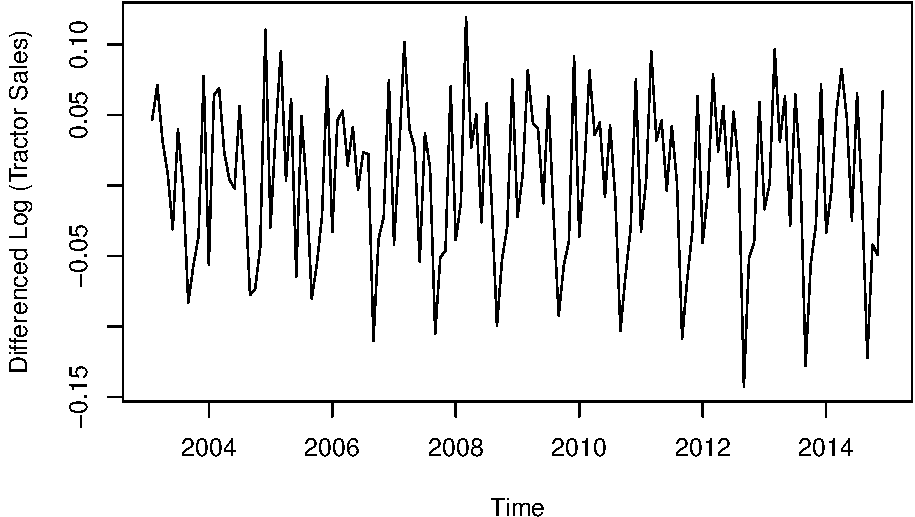
\includegraphics{_main_files/figure-latex/unnamed-chunk-66-1.pdf}

Find bedste model med auto.arima, når der er stationaritet.

Akaike Information Criterion (AIC) , og Bayesian Information Criterion (BIC), vælg ARIMA modellen med mindst AIC and BIC værdier. auto.arima finder den bedste model automatisk.

\begin{Shaded}
\begin{Highlighting}[]
\KeywordTok{require}\NormalTok{(forecast)}
\NormalTok{ARIMAfit =}\StringTok{ }\KeywordTok{auto.arima}\NormalTok{(}\KeywordTok{log10}\NormalTok{(data), }\DataTypeTok{approximation=}\OtherTok{FALSE}\NormalTok{,}\DataTypeTok{trace=}\OtherTok{FALSE}\NormalTok{)}
\NormalTok{ARIMAfit}
\end{Highlighting}
\end{Shaded}

\begin{verbatim}
## Series: log10(data) 
## ARIMA(0,1,1)(0,1,1)[12] 
## 
## Coefficients:
##           ma1     sma1
##       -0.4047  -0.5529
## s.e.   0.0885   0.0734
## 
## sigma^2 estimated as 0.0002571:  log likelihood=354.4
## AIC=-702.79   AICc=-702.6   BIC=-694.17
\end{verbatim}

Nu kan vi forudsige kommende traktor salg med modellen

\begin{Shaded}
\begin{Highlighting}[]
\KeywordTok{par}\NormalTok{(}\DataTypeTok{mfrow =} \KeywordTok{c}\NormalTok{(}\DecValTok{1}\NormalTok{,}\DecValTok{1}\NormalTok{))}
\NormalTok{pred =}\StringTok{ }\KeywordTok{predict}\NormalTok{(ARIMAfit, }\DataTypeTok{n.ahead =} \DecValTok{36}\NormalTok{)}
\NormalTok{salg <-}\StringTok{ }\DecValTok{10}\OperatorTok{^}\NormalTok{pred}\OperatorTok{$}\NormalTok{pred}
\NormalTok{salg}
\end{Highlighting}
\end{Shaded}

\begin{verbatim}
##            Jan       Feb       Mar       Apr       May       Jun       Jul
## 2015  567.7645  566.4765  670.8226  758.9138  855.9482  817.2827  938.7239
## 2016  625.2464  623.8280  738.7384  835.7481  942.6065  900.0265 1033.7626
## 2017  688.5479  686.9859  813.5300  920.3613 1038.0383  991.1474 1138.4233
##            Aug       Sep       Oct       Nov       Dec
## 2015  934.5120  703.5005  626.9879  571.9988  668.5363
## 2016 1029.1243  774.7246  690.4657  629.9094  736.2206
## 2017 1133.3154  853.1596  760.3701  693.6830  810.7573
\end{verbatim}

\begin{Shaded}
\begin{Highlighting}[]
\KeywordTok{plot}\NormalTok{(data,}\DataTypeTok{type=}\StringTok{'l'}\NormalTok{,}\DataTypeTok{xlim=}\KeywordTok{c}\NormalTok{(}\DecValTok{2003}\NormalTok{,}\DecValTok{2018}\NormalTok{),}\DataTypeTok{ylim=}\KeywordTok{c}\NormalTok{(}\DecValTok{1}\NormalTok{,}\DecValTok{1600}\NormalTok{),}\DataTypeTok{xlab =} \StringTok{'Year'}\NormalTok{,}\DataTypeTok{ylab =} \StringTok{'Tractor Salg'}\NormalTok{)}
\KeywordTok{lines}\NormalTok{(}\DecValTok{10}\OperatorTok{^}\NormalTok{(pred}\OperatorTok{$}\NormalTok{pred),}\DataTypeTok{col=}\StringTok{'blue'}\NormalTok{)}
\KeywordTok{lines}\NormalTok{(}\DecValTok{10}\OperatorTok{^}\NormalTok{(pred}\OperatorTok{$}\NormalTok{pred}\OperatorTok{+}\DecValTok{2}\OperatorTok{*}\NormalTok{pred}\OperatorTok{$}\NormalTok{se),}\DataTypeTok{col=}\StringTok{'orange'}\NormalTok{)}
\KeywordTok{lines}\NormalTok{(}\DecValTok{10}\OperatorTok{^}\NormalTok{(pred}\OperatorTok{$}\NormalTok{pred}\DecValTok{-2}\OperatorTok{*}\NormalTok{pred}\OperatorTok{$}\NormalTok{se),}\DataTypeTok{col=}\StringTok{'orange'}\NormalTok{)}
\end{Highlighting}
\end{Shaded}

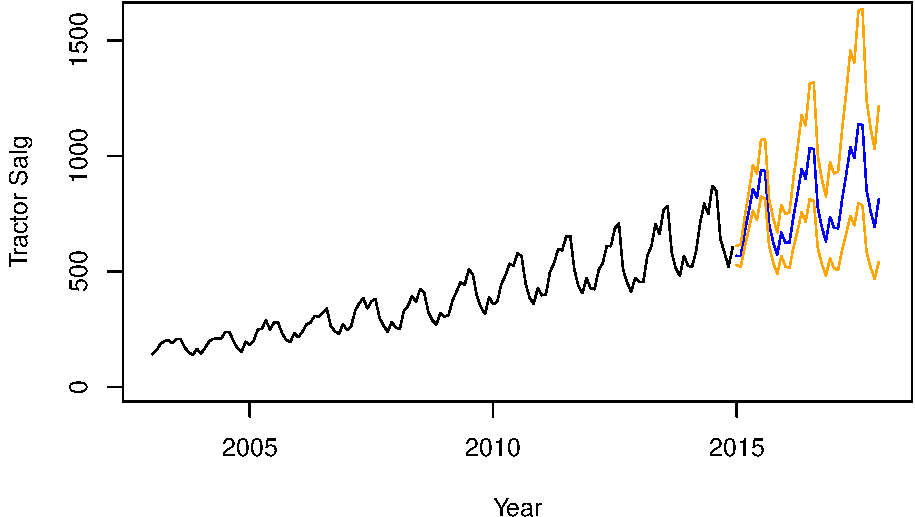
\includegraphics{_main_files/figure-latex/unnamed-chunk-68-1.pdf}

\hypertarget{detail-debet-card-forbrug-pa-island-millioner-isk.}{%
\subsection{Detail debet card forbrug på Island (millioner ISK).}\label{detail-debet-card-forbrug-pa-island-millioner-isk.}}

\begin{Shaded}
\begin{Highlighting}[]
\CommentTok{#Hent fpp pakken og load den}
\KeywordTok{plot}\NormalTok{(debitcards)}
\end{Highlighting}
\end{Shaded}

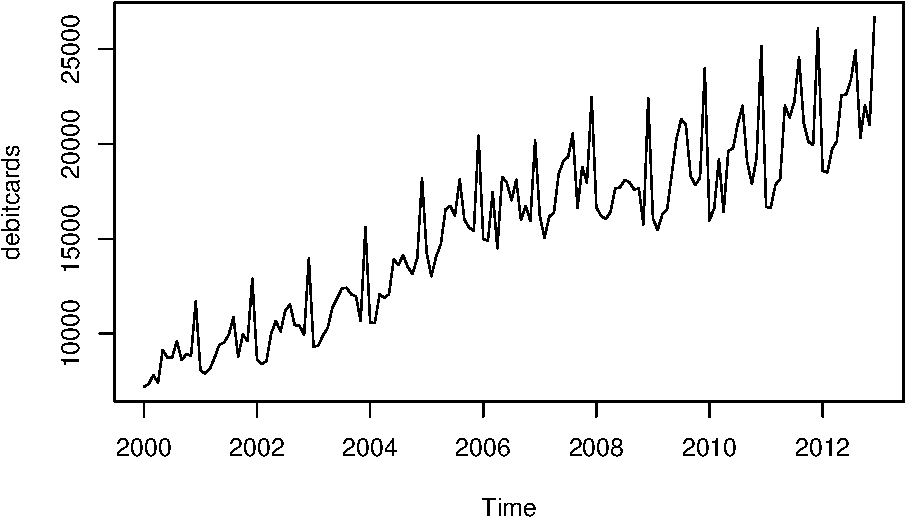
\includegraphics{_main_files/figure-latex/unnamed-chunk-70-1.pdf}

\begin{Shaded}
\begin{Highlighting}[]
\NormalTok{dldebitcards <-}\StringTok{ }\KeywordTok{diff}\NormalTok{(}\KeywordTok{log10}\NormalTok{(debitcards))}
\KeywordTok{plot}\NormalTok{(dldebitcards,}\DataTypeTok{ylab=}\StringTok{"Differenced Log (debitcards)"}\NormalTok{)}
\end{Highlighting}
\end{Shaded}

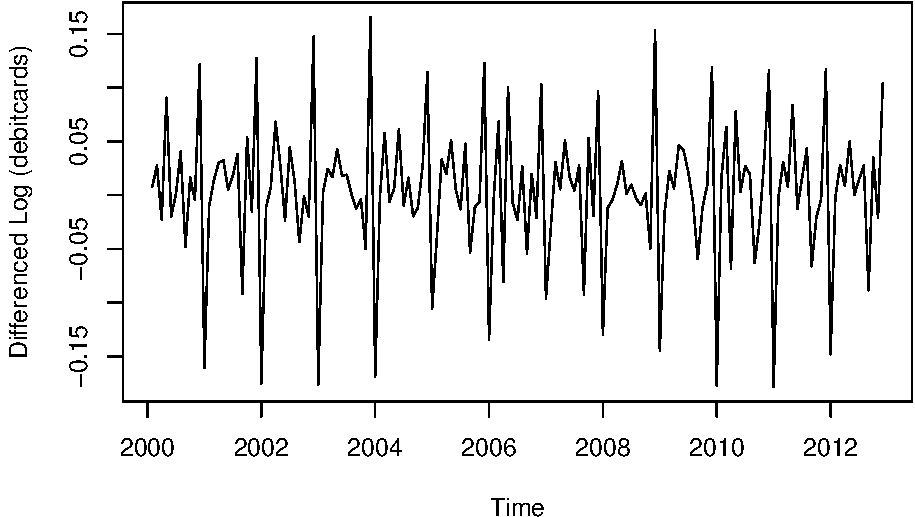
\includegraphics{_main_files/figure-latex/unnamed-chunk-71-1.pdf}

\begin{Shaded}
\begin{Highlighting}[]
\KeywordTok{require}\NormalTok{(forecast)}
\NormalTok{ARIMAfit =}\StringTok{ }\KeywordTok{auto.arima}\NormalTok{(}\KeywordTok{log10}\NormalTok{(debitcards), }\DataTypeTok{approximation=}\OtherTok{FALSE}\NormalTok{,}\DataTypeTok{trace=}\OtherTok{FALSE}\NormalTok{)}
\NormalTok{ARIMAfit}
\end{Highlighting}
\end{Shaded}

\begin{verbatim}
## Series: log10(debitcards) 
## ARIMA(2,1,0)(0,1,1)[12] 
## 
## Coefficients:
##           ar1      ar2     sma1
##       -0.7167  -0.4372  -0.8352
## s.e.   0.0761   0.0763   0.1085
## 
## sigma^2 estimated as 0.0004402:  log likelihood=343.95
## AIC=-679.9   AICc=-679.61   BIC=-668.05
\end{verbatim}

Nu kan vi forudsige kommende debetkort omsætning med modellen

\begin{Shaded}
\begin{Highlighting}[]
\KeywordTok{par}\NormalTok{(}\DataTypeTok{mfrow =} \KeywordTok{c}\NormalTok{(}\DecValTok{1}\NormalTok{,}\DecValTok{1}\NormalTok{))}
\NormalTok{pred =}\StringTok{ }\KeywordTok{predict}\NormalTok{(ARIMAfit, }\DataTypeTok{n.ahead =} \DecValTok{36}\NormalTok{)}
\KeywordTok{plot}\NormalTok{(debitcards,}\DataTypeTok{type=}\StringTok{'l'}\NormalTok{,}\DataTypeTok{xlim=}\KeywordTok{c}\NormalTok{(}\DecValTok{2000}\NormalTok{,}\DecValTok{2016}\NormalTok{),}\DataTypeTok{ylim=}\KeywordTok{c}\NormalTok{(}\DecValTok{1}\NormalTok{,}\DecValTok{40000}\NormalTok{),}\DataTypeTok{xlab =} \StringTok{'Year'}\NormalTok{,}\DataTypeTok{ylab =} \StringTok{'Debetcard usage'}\NormalTok{)}
\KeywordTok{lines}\NormalTok{(}\DecValTok{10}\OperatorTok{^}\NormalTok{(pred}\OperatorTok{$}\NormalTok{pred),}\DataTypeTok{col=}\StringTok{'blue'}\NormalTok{)}
\KeywordTok{lines}\NormalTok{(}\DecValTok{10}\OperatorTok{^}\NormalTok{(pred}\OperatorTok{$}\NormalTok{pred}\OperatorTok{+}\DecValTok{2}\OperatorTok{*}\NormalTok{pred}\OperatorTok{$}\NormalTok{se),}\DataTypeTok{col=}\StringTok{'orange'}\NormalTok{)}
\KeywordTok{lines}\NormalTok{(}\DecValTok{10}\OperatorTok{^}\NormalTok{(pred}\OperatorTok{$}\NormalTok{pred}\DecValTok{-2}\OperatorTok{*}\NormalTok{pred}\OperatorTok{$}\NormalTok{se),}\DataTypeTok{col=}\StringTok{'orange'}\NormalTok{)}
\end{Highlighting}
\end{Shaded}

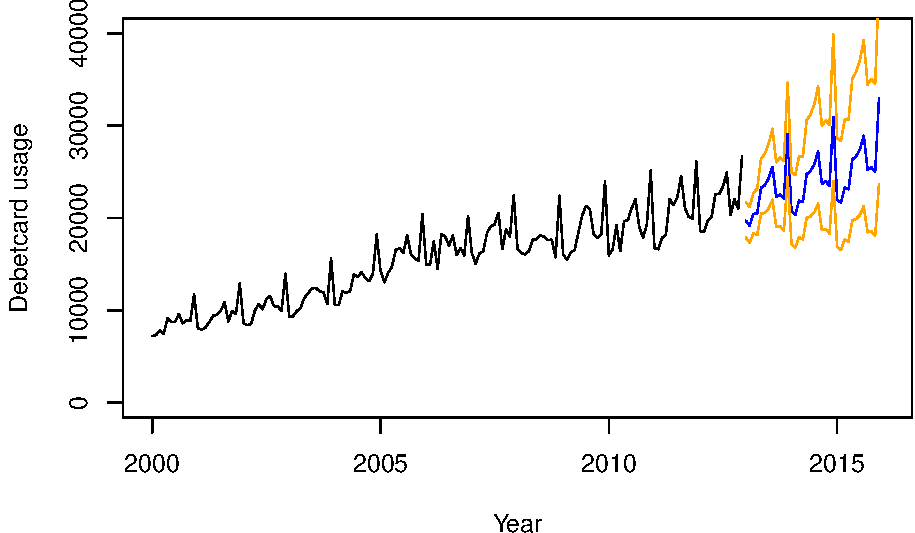
\includegraphics{_main_files/figure-latex/unnamed-chunk-73-1.pdf}

Forudsagt brug af debetkort bliver:

\begin{Shaded}
\begin{Highlighting}[]
\DecValTok{10}\OperatorTok{^}\NormalTok{(pred}\OperatorTok{$}\NormalTok{pred)}
\end{Highlighting}
\end{Shaded}

\begin{verbatim}
##           Jan      Feb      Mar      Apr      May      Jun      Jul
## 2013 19717.77 19162.87 20436.29 20506.84 23262.14 23545.62 24292.86
## 2014 20701.39 20352.57 21886.85 21721.53 24745.18 25091.09 25806.49
## 2015 22017.60 21649.95 23281.85 23104.56 26321.98 26689.74 27450.29
##           Aug      Sep      Oct      Nov      Dec
## 2013 25544.16 22267.47 22543.80 22081.63 29090.93
## 2014 27175.65 23697.15 23970.40 23490.36 30947.83
## 2015 28907.08 25206.87 25497.43 24986.92 32919.46
\end{verbatim}

\hypertarget{forecast-aktiekurser}{%
\section{Forecast Aktiekurser}\label{forecast-aktiekurser}}

Man kan hente online aktiekurser med quantmod pakken installer denne med fx. pacman, vi skal også bruge pakken forecast som vi ligeledes henter. Vi henter nedenfor Google justeret lukkekurs til dato det er 6 søjle i GOOG matricen nedenfor. Vi kan se forecaste aktiekursen vha.

\begin{Shaded}
\begin{Highlighting}[]
\NormalTok{pacman}\OperatorTok{::}\KeywordTok{p_load}\NormalTok{(quantmod, forecast)}
\KeywordTok{getSymbols}\NormalTok{(}\StringTok{"GOOG"}\NormalTok{,}\DataTypeTok{from =} \StringTok{"2017-01-01"}\NormalTok{, }\DataTypeTok{to =} \KeywordTok{Sys.Date}\NormalTok{(),}\DataTypeTok{getSymbols.warning4.0=}\OtherTok{FALSE}\NormalTok{)}
\end{Highlighting}
\end{Shaded}

\begin{verbatim}
## [1] "GOOG"
\end{verbatim}

\begin{Shaded}
\begin{Highlighting}[]
\KeywordTok{plot}\NormalTok{(GOOG[,}\DecValTok{6}\NormalTok{],}\DataTypeTok{main =} \StringTok{"Google adj. close"}\NormalTok{)}
\end{Highlighting}
\end{Shaded}

\includegraphics{_main_files/figure-latex/unnamed-chunk-76-1.pdf}

\begin{Shaded}
\begin{Highlighting}[]
\NormalTok{agoog <-}\StringTok{ }\KeywordTok{auto.arima}\NormalTok{(GOOG[,}\DecValTok{6}\NormalTok{])}
\NormalTok{agoog}
\end{Highlighting}
\end{Shaded}

\begin{verbatim}
## Series: GOOG[, 6] 
## ARIMA(0,1,0) 
## 
## sigma^2 estimated as 227.3:  log likelihood=-2400.69
## AIC=4803.39   AICc=4803.4   BIC=4807.75
\end{verbatim}

\begin{Shaded}
\begin{Highlighting}[]
\NormalTok{fagoog <-}\StringTok{ }\KeywordTok{forecast}\NormalTok{(agoog)}
\NormalTok{fagoog}
\end{Highlighting}
\end{Shaded}

\begin{verbatim}
##     Point Forecast    Lo 80    Hi 80    Lo 95    Hi 95
## 583        1272.18 1252.860 1291.500 1242.633 1301.727
## 584        1272.18 1244.857 1299.503 1230.394 1313.966
## 585        1272.18 1238.717 1305.643 1221.003 1323.358
## 586        1272.18 1233.540 1310.820 1213.085 1331.275
## 587        1272.18 1228.979 1315.381 1206.110 1338.250
## 588        1272.18 1224.856 1319.504 1199.804 1344.556
## 589        1272.18 1221.064 1323.296 1194.005 1350.355
## 590        1272.18 1217.535 1326.825 1188.608 1355.753
## 591        1272.18 1214.220 1330.140 1183.538 1360.822
## 592        1272.18 1211.085 1333.275 1178.743 1365.617
\end{verbatim}

\begin{Shaded}
\begin{Highlighting}[]
\KeywordTok{plot}\NormalTok{(fagoog,}\DataTypeTok{main =} \StringTok{"Google adj. close"}\NormalTok{)}
\end{Highlighting}
\end{Shaded}

\includegraphics{_main_files/figure-latex/unnamed-chunk-77-1.pdf}

\begin{Shaded}
\begin{Highlighting}[]
\KeywordTok{getSymbols}\NormalTok{(}\StringTok{"GS"}\NormalTok{,}\DataTypeTok{from =} \StringTok{"2017-01-01"}\NormalTok{, }\DataTypeTok{to =} \KeywordTok{Sys.Date}\NormalTok{(),}\DataTypeTok{getSymbols.warning4.0=}\OtherTok{FALSE}\NormalTok{)}
\end{Highlighting}
\end{Shaded}

\begin{verbatim}
## [1] "GS"
\end{verbatim}

\begin{Shaded}
\begin{Highlighting}[]
\KeywordTok{plot}\NormalTok{(GS[,}\DecValTok{6}\NormalTok{],}\DataTypeTok{main =} \StringTok{"Goldman Sachs adj. close"}\NormalTok{)}
\end{Highlighting}
\end{Shaded}

\includegraphics{_main_files/figure-latex/unnamed-chunk-78-1.pdf}

\begin{Shaded}
\begin{Highlighting}[]
\NormalTok{ags <-}\StringTok{ }\KeywordTok{auto.arima}\NormalTok{(GS[,}\DecValTok{6}\NormalTok{])}
\NormalTok{ags}
\end{Highlighting}
\end{Shaded}

\begin{verbatim}
## Series: GS[, 6] 
## ARIMA(0,1,0) 
## 
## sigma^2 estimated as 10.68:  log likelihood=-1512.31
## AIC=3026.62   AICc=3026.62   BIC=3030.98
\end{verbatim}

\begin{Shaded}
\begin{Highlighting}[]
\NormalTok{fags <-}\StringTok{ }\KeywordTok{forecast}\NormalTok{(ags)}
\NormalTok{fags}
\end{Highlighting}
\end{Shaded}

\begin{verbatim}
##     Point Forecast    Lo 80    Hi 80    Lo 95    Hi 95
## 583         203.08 198.8926 207.2674 196.6759 209.4841
## 584         203.08 197.1581 209.0019 194.0233 212.1367
## 585         203.08 195.8272 210.3328 191.9879 214.1722
## 586         203.08 194.7052 211.4548 190.2719 215.8881
## 587         203.08 193.7167 212.4433 188.7601 217.3999
## 588         203.08 192.8230 213.3370 187.3933 218.7667
## 589         203.08 192.0012 214.1588 186.1365 220.0235
## 590         203.08 191.2363 214.9237 184.9666 221.1934
## 591         203.08 190.5178 215.6422 183.8678 222.2922
## 592         203.08 189.8383 216.3217 182.8286 223.3314
\end{verbatim}

\begin{Shaded}
\begin{Highlighting}[]
\KeywordTok{plot}\NormalTok{(fags,}\DataTypeTok{main =} \StringTok{"Goldman Sachs adj. close"}\NormalTok{)}
\end{Highlighting}
\end{Shaded}

\includegraphics{_main_files/figure-latex/unnamed-chunk-78-2.pdf}

\begin{Shaded}
\begin{Highlighting}[]
\KeywordTok{getSymbols}\NormalTok{(}\StringTok{"DANSKE.CO"}\NormalTok{,}\DataTypeTok{from =} \StringTok{"2017-01-01"}\NormalTok{, }\DataTypeTok{to =} \KeywordTok{Sys.Date}\NormalTok{(),}\DataTypeTok{getSymbols.warning4.0=}\OtherTok{FALSE}\NormalTok{)}
\end{Highlighting}
\end{Shaded}

\begin{verbatim}
## [1] "DANSKE.CO"
\end{verbatim}

\begin{Shaded}
\begin{Highlighting}[]
\KeywordTok{plot}\NormalTok{(DANSKE.CO[,}\DecValTok{6}\NormalTok{],}\DataTypeTok{main =} \StringTok{"Danske Bank adj. close"}\NormalTok{)}
\end{Highlighting}
\end{Shaded}

\includegraphics{_main_files/figure-latex/unnamed-chunk-79-1.pdf}

\begin{Shaded}
\begin{Highlighting}[]
\NormalTok{addb <-}\StringTok{ }\KeywordTok{auto.arima}\NormalTok{(DANSKE.CO[,}\DecValTok{6}\NormalTok{])}
\NormalTok{addb}
\end{Highlighting}
\end{Shaded}

\begin{verbatim}
## Series: DANSKE.CO[, 6] 
## ARIMA(1,2,2) 
## 
## Coefficients:
##           ar1      ma1      ma2
##       -0.2609  -0.8131  -0.1748
## s.e.   0.3035   0.3082   0.3057
## 
## sigma^2 estimated as 6.441:  log likelihood=-1356.64
## AIC=2721.28   AICc=2721.35   BIC=2738.71
\end{verbatim}

\begin{Shaded}
\begin{Highlighting}[]
\NormalTok{faddb <-}\StringTok{ }\KeywordTok{forecast}\NormalTok{(addb)}
\NormalTok{faddb}
\end{Highlighting}
\end{Shaded}

\begin{verbatim}
##     Point Forecast    Lo 80    Hi 80    Lo 95    Hi 95
## 580       128.2108 124.9582 131.4633 123.2364 133.1851
## 581       128.1523 123.7194 132.5851 121.3728 134.9317
## 582       128.0335 122.6163 133.4508 119.7486 136.3185
## 583       127.9306 121.6758 134.1853 118.3648 137.4963
## 584       127.8235 120.8147 134.8323 117.1044 138.5425
## 585       127.7174 120.0158 135.4190 115.9388 139.4960
## 586       127.6111 119.2620 135.9603 114.8422 140.3800
## 587       127.5049 118.5437 136.4661 113.7999 141.2098
## 588       127.3986 117.8539 136.9433 112.8013 141.9960
## 589       127.2924 117.1877 137.3971 111.8385 142.7462
\end{verbatim}

\begin{Shaded}
\begin{Highlighting}[]
\KeywordTok{plot}\NormalTok{(faddb,}\DataTypeTok{main =} \StringTok{"Danske Bank adj. close"}\NormalTok{)}
\end{Highlighting}
\end{Shaded}

\includegraphics{_main_files/figure-latex/unnamed-chunk-79-2.pdf}

\begin{Shaded}
\begin{Highlighting}[]
\KeywordTok{getSymbols}\NormalTok{(}\StringTok{"BRK-A"}\NormalTok{,}\DataTypeTok{from =} \StringTok{"2000-01-01"}\NormalTok{, }\DataTypeTok{to =} \KeywordTok{Sys.Date}\NormalTok{(),}\DataTypeTok{getSymbols.warning4.0=}\OtherTok{FALSE}\NormalTok{)}
\end{Highlighting}
\end{Shaded}

\begin{verbatim}
## [1] "BRK-A"
\end{verbatim}

\begin{Shaded}
\begin{Highlighting}[]
\KeywordTok{plot}\NormalTok{(}\StringTok{`}\DataTypeTok{BRK-A}\StringTok{`}\NormalTok{[,}\DecValTok{6}\NormalTok{],}\DataTypeTok{main =} \StringTok{"Berkshire adj. close"}\NormalTok{)}
\end{Highlighting}
\end{Shaded}

\includegraphics{_main_files/figure-latex/unnamed-chunk-80-1.pdf}

\begin{Shaded}
\begin{Highlighting}[]
\NormalTok{aberkshire <-}\StringTok{ }\KeywordTok{auto.arima}\NormalTok{(}\StringTok{`}\DataTypeTok{BRK-A}\StringTok{`}\NormalTok{[,}\DecValTok{6}\NormalTok{])}
\NormalTok{aberkshire}
\end{Highlighting}
\end{Shaded}

\begin{verbatim}
## Series: `BRK-A`[, 6] 
## ARIMA(3,1,4) with drift 
## 
## Coefficients:
##          ar1      ar2     ar3      ma1     ma2      ma3      ma4    drift
##       0.9581  -0.8520  0.4078  -0.9895  0.8649  -0.4151  -0.0742  53.6558
## s.e.  0.4050   0.7223  0.4820   0.4055  0.7413   0.5257   0.0519  20.8218
## 
## sigma^2 estimated as 3341081:  log likelihood=-43377.2
## AIC=86772.4   AICc=86772.44   BIC=86830.8
\end{verbatim}

\begin{Shaded}
\begin{Highlighting}[]
\NormalTok{faberkshire <-}\StringTok{ }\KeywordTok{forecast}\NormalTok{(aberkshire)}
\NormalTok{faberkshire}
\end{Highlighting}
\end{Shaded}

\begin{verbatim}
##      Point Forecast    Lo 80    Hi 80    Lo 95    Hi 95
## 4860       320636.1 318293.6 322978.6 317053.6 324218.6
## 4861       320499.4 317238.1 323760.7 315511.7 325487.1
## 4862       320499.6 316549.4 324449.8 314458.3 326540.9
## 4863       320307.1 315767.9 324846.3 313365.0 327249.2
## 4864       320092.8 315102.5 325083.1 312460.8 327724.8
## 4865       320077.6 314739.7 325415.6 311914.0 328241.3
## 4866       320193.3 314538.8 325847.9 311545.4 328841.2
## 4867       320255.7 314283.1 326228.3 311121.4 329390.0
## 4868       320236.8 313960.0 326513.7 310637.2 329836.4
## 4869       320238.8 313687.5 326790.2 310219.5 330258.2
\end{verbatim}

\begin{Shaded}
\begin{Highlighting}[]
\KeywordTok{plot}\NormalTok{(faberkshire,}\DataTypeTok{main =} \StringTok{"Berkshire adj. close"}\NormalTok{)}
\end{Highlighting}
\end{Shaded}

\includegraphics{_main_files/figure-latex/unnamed-chunk-80-2.pdf}

\hypertarget{aktieafkast}{%
\section{Aktieafkast}\label{aktieafkast}}

I Quantmod pakken ligger også mulighed for at beregne fx. dagligt, ugentligt afkast, dette gør vi vha. funktionen ``periodReturn''.

\begin{Shaded}
\begin{Highlighting}[]
\KeywordTok{getSymbols}\NormalTok{(}\StringTok{"AAPL"}\NormalTok{,}\DataTypeTok{src=}\StringTok{'yahoo'}\NormalTok{)}
\end{Highlighting}
\end{Shaded}

\begin{verbatim}
## [1] "AAPL"
\end{verbatim}

\begin{Shaded}
\begin{Highlighting}[]
\NormalTok{apple <-}\StringTok{ }\KeywordTok{periodReturn}\NormalTok{(}\StringTok{`}\DataTypeTok{AAPL}\StringTok{`}\NormalTok{,}\DataTypeTok{period=}\StringTok{'yearly'}\NormalTok{,}\DataTypeTok{subset=}\StringTok{'2003::'}\NormalTok{)  }\CommentTok{# Årligt Afkast 2003 til i dag}
\KeywordTok{plot}\NormalTok{(apple, }\DataTypeTok{main =} \StringTok{"Apple årligt afkast siden 2007"}\NormalTok{)}
\end{Highlighting}
\end{Shaded}

\includegraphics{_main_files/figure-latex/unnamed-chunk-81-1.pdf}

\begin{Shaded}
\begin{Highlighting}[]
\KeywordTok{auto.arima}\NormalTok{(apple)}
\end{Highlighting}
\end{Shaded}

\begin{verbatim}
## Series: apple 
## ARIMA(1,0,0) with non-zero mean 
## 
## Coefficients:
##           ar1    mean
##       -0.5894  0.3165
## s.e.   0.2455  0.0783
## 
## sigma^2 estimated as 0.2222:  log likelihood=-7.8
## AIC=21.59   AICc=24.26   BIC=23.29
\end{verbatim}

\begin{Shaded}
\begin{Highlighting}[]
\KeywordTok{getSymbols}\NormalTok{(}\StringTok{"BRK-A"}\NormalTok{,}\DataTypeTok{src=}\StringTok{'yahoo'}\NormalTok{)}
\end{Highlighting}
\end{Shaded}

\begin{verbatim}
## [1] "BRK-A"
\end{verbatim}

\begin{Shaded}
\begin{Highlighting}[]
\NormalTok{berkshire <-}\StringTok{ }\KeywordTok{periodReturn}\NormalTok{(}\StringTok{`}\DataTypeTok{BRK-A}\StringTok{`}\NormalTok{,}\DataTypeTok{period=}\StringTok{'yearly'}\NormalTok{,}\DataTypeTok{subset=}\StringTok{'2003::'}\NormalTok{)}
\KeywordTok{plot}\NormalTok{(berkshire, }\DataTypeTok{main =} \StringTok{"Berkshire årligt afkast siden 2007"}\NormalTok{)}
\end{Highlighting}
\end{Shaded}

\includegraphics{_main_files/figure-latex/unnamed-chunk-82-1.pdf}

\begin{Shaded}
\begin{Highlighting}[]
\KeywordTok{auto.arima}\NormalTok{(berkshire)}
\end{Highlighting}
\end{Shaded}

\begin{verbatim}
## Series: berkshire 
## ARIMA(0,0,0) with non-zero mean 
## 
## Coefficients:
##         mean
##       0.1023
## s.e.  0.0501
## 
## sigma^2 estimated as 0.0353:  log likelihood=3.81
## AIC=-3.62   AICc=-2.42   BIC=-2.49
\end{verbatim}

\hypertarget{arima-opsamling-video}{%
\subsection{ARIMA opsamling video}\label{arima-opsamling-video}}

\hypertarget{deskriptiv-statistik}{%
\chapter{Deskriptiv statistik}\label{deskriptiv-statistik}}

\hypertarget{videoer-teori}{%
\section{Videoer teori}\label{videoer-teori}}

\hypertarget{introduktion}{%
\subsubsection{Introduktion}\label{introduktion}}

\hypertarget{data}{%
\subsubsection{Data}\label{data}}

\hypertarget{deskriptiv-statistik-1}{%
\subsubsection{Deskriptiv statistik}\label{deskriptiv-statistik-1}}

\hypertarget{fraktiler}{%
\subsubsection{Fraktiler}\label{fraktiler}}

\hypertarget{skvhed}{%
\subsubsection{Skævhed}\label{skvhed}}

\hypertarget{kurtosis}{%
\subsubsection{Kurtosis}\label{kurtosis}}

\hypertarget{sandsynligheder}{%
\subsubsection{Sandsynligheder}\label{sandsynligheder}}

\hypertarget{normalfordelingen}{%
\subsubsection{Normalfordelingen}\label{normalfordelingen}}

\hypertarget{konfidensintervaller-normalfordelingen}{%
\subsubsection{Konfidensintervaller normalfordelingen}\label{konfidensintervaller-normalfordelingen}}

\hypertarget{normalfraktildiagram}{%
\subsubsection{Normalfraktildiagram}\label{normalfraktildiagram}}

\hypertarget{stikprvefordelingen}{%
\subsubsection{Stikprøvefordelingen}\label{stikprvefordelingen}}

\hypertarget{stikprvefordelingen-2}{%
\subsubsection{Stikprøvefordelingen 2}\label{stikprvefordelingen-2}}

\hypertarget{parameter-estimat}{%
\subsubsection{Parameter-estimat}\label{parameter-estimat}}

\hypertarget{t-fordelingen}{%
\subsubsection{t-fordelingen}\label{t-fordelingen}}

\hypertarget{konfidensinterval-middelvrdien}{%
\subsubsection{Konfidensinterval middelværdien}\label{konfidensinterval-middelvrdien}}

\hypertarget{fejlmargin}{%
\subsubsection{Fejlmargin}\label{fejlmargin}}

\hypertarget{hypotesetest-middelvrdi}{%
\subsubsection{Hypotesetest middelværdi}\label{hypotesetest-middelvrdi}}

\hypertarget{liner-regression}{%
\subsubsection{Lineær regression}\label{liner-regression}}

\hypertarget{liner-regression-forudstninger}{%
\subsubsection{Lineær regression forudsætninger}\label{liner-regression-forudstninger}}

\hypertarget{goodness-of-fit-test-1}{%
\subsubsection{Goodness of fit test}\label{goodness-of-fit-test-1}}

\hypertarget{chi-i-anden-test-1}{%
\subsection{Chi i anden test}\label{chi-i-anden-test-1}}

\hypertarget{chi-i-anden-test-2}{%
\subsection{Chi i anden test 2}\label{chi-i-anden-test-2}}

\hypertarget{anova-1}{%
\subsection{Anova}\label{anova-1}}

\hypertarget{freestat-fin}{%
\section{Freestat FIN}\label{freestat-fin}}

\hypertarget{mindmap-hypoteser}{%
\subsubsection{Mindmap hypoteser}\label{mindmap-hypoteser}}

\hypertarget{beskrivende-statistik-freestat}{%
\subsubsection{Beskrivende statistik Freestat}\label{beskrivende-statistik-freestat}}

\hypertarget{middelvrdi-standardafvigelse-ki}{%
\subsubsection{Middelværdi standardafvigelse KI}\label{middelvrdi-standardafvigelse-ki}}

\hypertarget{middelvrdi-test}{%
\subsubsection{Middelværdi test}\label{middelvrdi-test}}

\hypertarget{middelvrdi-fejlmargin}{%
\subsubsection{Middelværdi fejlmargin}\label{middelvrdi-fejlmargin}}

\hypertarget{standardafvigelse-test}{%
\subsubsection{Standardafvigelse test}\label{standardafvigelse-test}}

\hypertarget{andel-test-og-ki}{%
\subsubsection{1 Andel test og KI}\label{andel-test-og-ki}}

\hypertarget{andel-fejlmargin-og-fpc}{%
\subsubsection{1 Andel fejlmargin og FPC}\label{andel-fejlmargin-og-fpc}}

\hypertarget{fpc-endelig-populations-korrektion-og-z-test}{%
\subsubsection{FPC endelig populations korrektion og z-test}\label{fpc-endelig-populations-korrektion-og-z-test}}

\hypertarget{andel-test-og-ki-1}{%
\subsubsection{1 Andel test og KI}\label{andel-test-og-ki-1}}

\hypertarget{andel-fejlmargin-og-fpc-1}{%
\subsubsection{1 Andel fejlmargin og FPC}\label{andel-fejlmargin-og-fpc-1}}

\hypertarget{andele}{%
\subsubsection{2 Andele}\label{andele}}

\hypertarget{middelvrdier}{%
\subsubsection{2 Middelværdier}\label{middelvrdier}}

\hypertarget{parret-t-test}{%
\subsubsection{Parret t-test}\label{parret-t-test}}

\hypertarget{korrelation}{%
\subsubsection{Korrelation}\label{korrelation}}

\hypertarget{simpel-liner-regression}{%
\subsubsection{Simpel lineær regression}\label{simpel-liner-regression}}

\hypertarget{simpel-liner-regression-pi-og-ki}{%
\subsubsection{Simpel lineær regression PI og KI}\label{simpel-liner-regression-pi-og-ki}}

\hypertarget{multipel-liner-regression}{%
\subsubsection{Multipel lineær regression}\label{multipel-liner-regression}}

\hypertarget{dummy-variable}{%
\subsubsection{Dummy variable}\label{dummy-variable}}

\hypertarget{multipel-liner-regression-forudsagt-vrdi}{%
\subsubsection{Multipel lineær regression forudsagt værdi}\label{multipel-liner-regression-forudsagt-vrdi}}

\hypertarget{anova-variansanalyse}{%
\subsubsection{ANOVA variansanalyse}\label{anova-variansanalyse}}

\hypertarget{eksamensvideoer}{%
\section{Eksamensvideoer}\label{eksamensvideoer}}

\begin{center}\rule{0.5\linewidth}{\linethickness}\end{center}

\begin{center}\rule{0.5\linewidth}{\linethickness}\end{center}

\begin{center}\rule{0.5\linewidth}{\linethickness}\end{center}

\hypertarget{eksamen-statistik-2-timer-2017-9-5}{%
\subsubsection{Eksamen statistik 2 timer 2017 9 5}\label{eksamen-statistik-2-timer-2017-9-5}}

\href{https://www.dropbox.com/s/3gd6mcocowe8glq/2017\%209\%20Statistik\%20Fin.pdf?dl=1}{2017 9 5 Opgave}
\href{https://www.dropbox.com/s/y4p8j90wjbzhtb3/2017\%209\%20statistik\%20Data\%202.RE.xlsx?dl=1}{2017 9 5 Data}
\href{https://www.dropbox.com/s/wruqocv7g0fvkob/2017\%209\%20Statistik\%20Fin\%20opg\%201\%20og\%203\%20l\%C3\%B8sning\%20skabelon\%20Freestat\%20.docx?dl=1}{2017 9 5 Løsningsforslag}

\hypertarget{opgave-1-1-normalfraktildiagram}{%
\paragraph{Opgave 1 1 Normalfraktildiagram}\label{opgave-1-1-normalfraktildiagram}}

\hypertarget{opgave-1-2-test-middel}{%
\paragraph{Opgave 1 2 Test middel}\label{opgave-1-2-test-middel}}

\hypertarget{opgave-1-3-varianshomogenitet}{%
\paragraph{Opgave 1 3 Varianshomogenitet}\label{opgave-1-3-varianshomogenitet}}

\hypertarget{opgave-1-4-test-af-2-middelvrdier}{%
\paragraph{Opgave 1 4 Test af 2 middelværdier}\label{opgave-1-4-test-af-2-middelvrdier}}

\hypertarget{opgave-1-5-konfidensinterval-for-forskellen-af-middelvrdier}{%
\paragraph{Opgave 1 5 Konfidensinterval for forskellen af middelværdier}\label{opgave-1-5-konfidensinterval-for-forskellen-af-middelvrdier}}

\hypertarget{opgave-3-1-test-af-andel}{%
\paragraph{Opgave 3 1 Test af andel}\label{opgave-3-1-test-af-andel}}

\hypertarget{opgave-3-2-konfidensinterval-for-middelvrdi}{%
\paragraph{Opgave 3 2 Konfidensinterval for middelværdi}\label{opgave-3-2-konfidensinterval-for-middelvrdi}}

\begin{center}\rule{0.5\linewidth}{\linethickness}\end{center}

\begin{center}\rule{0.5\linewidth}{\linethickness}\end{center}

\begin{center}\rule{0.5\linewidth}{\linethickness}\end{center}

\begin{center}\rule{0.5\linewidth}{\linethickness}\end{center}

\begin{center}\rule{0.5\linewidth}{\linethickness}\end{center}

\begin{center}\rule{0.5\linewidth}{\linethickness}\end{center}

\hypertarget{eksamen-statistik-2-timer-2016-8-10}{%
\subsubsection{Eksamen statistik 2 timer 2016 8 10}\label{eksamen-statistik-2-timer-2016-8-10}}

\href{https://drive.google.com/uc?export=download\&id=0B1E7VnhxsDMlTy1NVjFBMDRLZFk}{2016 8 10 Opgave}
\href{https://drive.google.com/uc?export=download\&id=0B1E7VnhxsDMlcVdQUVFjUEp2SUE}{2016 8 10 Data}
\href{https://drive.google.com/uc?export=download\&id=0B1E7VnhxsDMlQnNjMk9XZDZKWUU}{2016 8 10 Løsningsforslag}

\hypertarget{opgave-1-liner-regression}{%
\paragraph{Opgave 1 Lineær regression}\label{opgave-1-liner-regression}}

\hypertarget{opgave-2-andele}{%
\paragraph{Opgave 2 Andele}\label{opgave-2-andele}}

\hypertarget{opgave-3-middelvrdier}{%
\paragraph{Opgave 3 Middelværdier}\label{opgave-3-middelvrdier}}

\hypertarget{opgave-4-teori-ki-punktestimat-testniveau}{%
\paragraph{Opgave 4 Teori KI, punktestimat, testniveau}\label{opgave-4-teori-ki-punktestimat-testniveau}}

\begin{center}\rule{0.5\linewidth}{\linethickness}\end{center}

\begin{center}\rule{0.5\linewidth}{\linethickness}\end{center}

\begin{center}\rule{0.5\linewidth}{\linethickness}\end{center}

\begin{center}\rule{0.5\linewidth}{\linethickness}\end{center}

\begin{center}\rule{0.5\linewidth}{\linethickness}\end{center}

\begin{center}\rule{0.5\linewidth}{\linethickness}\end{center}

\hypertarget{eksamen-statistik-2-timer-2015-8-7}{%
\subsubsection{Eksamen statistik 2 timer 2015 8 7}\label{eksamen-statistik-2-timer-2015-8-7}}

\href{https://www.dropbox.com/s/dwbpp3ykq17tbvb/2015\%208\%207\%201.reeksamen.pdf?dl=1}{2015 8 7 Opgave}
\href{https://www.dropbox.com/s/45d1xkhjp3c0owh/2015\%208\%207\%20Data.xlsx?dl=1}{2015 8 7 Data}
\href{https://www.dropbox.com/s/9nhbc21yth3si6o/2015\%208\%207\%20Freestat\%20skabelon\%20l\%C3\%B8sning.docx?dl=1}{2015 8 7 Løsningsforslag}

\hypertarget{opgave-1.1}{%
\paragraph{Opgave 1.1}\label{opgave-1.1}}

\hypertarget{opgave-1.2}{%
\paragraph{Opgave 1.2}\label{opgave-1.2}}

\hypertarget{opgave-1.3}{%
\paragraph{Opgave 1.3}\label{opgave-1.3}}

\hypertarget{opgave-1.4}{%
\paragraph{Opgave 1.4}\label{opgave-1.4}}

\hypertarget{opgave-1.5}{%
\paragraph{Opgave 1.5}\label{opgave-1.5}}

\hypertarget{opgave-2.1-og-2.2}{%
\paragraph{Opgave 2.1 og 2.2}\label{opgave-2.1-og-2.2}}

\hypertarget{opgave-2.3}{%
\paragraph{Opgave 2.3}\label{opgave-2.3}}

\hypertarget{opgave-3.1}{%
\paragraph{Opgave 3.1}\label{opgave-3.1}}

\hypertarget{opgave-3.2}{%
\paragraph{Opgave 3.2}\label{opgave-3.2}}

\hypertarget{opgave-3.3}{%
\paragraph{Opgave 3.3}\label{opgave-3.3}}

\begin{center}\rule{0.5\linewidth}{\linethickness}\end{center}

\begin{center}\rule{0.5\linewidth}{\linethickness}\end{center}

\begin{center}\rule{0.5\linewidth}{\linethickness}\end{center}

\begin{center}\rule{0.5\linewidth}{\linethickness}\end{center}

\begin{center}\rule{0.5\linewidth}{\linethickness}\end{center}

\begin{center}\rule{0.5\linewidth}{\linethickness}\end{center}

\hypertarget{eksamen-statistik-2-timer-2015-3-4}{%
\subsubsection{Eksamen statistik 2 timer 2015 3 4}\label{eksamen-statistik-2-timer-2015-3-4}}

\href{https://drive.google.com/file/d/0B1E7VnhxsDMlLVBMek5kWEhRZlU/view?usp=sharing}{2015 3 4 Opgave}
\href{https://drive.google.com/file/d/0B1E7VnhxsDMlX0p3Qk8wWlNxM28/view?usp=sharing}{2015 3 4 Data}
\href{https://drive.google.com/file/d/0B1E7VnhxsDMlWXNWTW55Sk94RDA/view?usp=sharing}{2015 3 4 Løsningsforslag}

\hypertarget{opgave-1-liner-regression-1}{%
\paragraph{Opgave 1 lineær regression}\label{opgave-1-liner-regression-1}}

\hypertarget{opgave-2-test-af-2-middelvrdier}{%
\paragraph{Opgave 2 Test af 2 middelværdier}\label{opgave-2-test-af-2-middelvrdier}}

\hypertarget{opgave-3-ki-andel-og-middel-test-af-middel}{%
\paragraph{Opgave 3 KI andel og middel, test af middel}\label{opgave-3-ki-andel-og-middel-test-af-middel}}

\hypertarget{opgave-4-2-andele}{%
\paragraph{Opgave 4 2 Andele}\label{opgave-4-2-andele}}

\hypertarget{eksamensvideoer-au-smartlearning}{%
\section{Eksamensvideoer AU Smartlearning}\label{eksamensvideoer-au-smartlearning}}

\begin{center}\rule{0.5\linewidth}{\linethickness}\end{center}

\begin{center}\rule{0.5\linewidth}{\linethickness}\end{center}

\begin{center}\rule{0.5\linewidth}{\linethickness}\end{center}

\hypertarget{konverter-eksamensopgaven-til-word}{%
\subsubsection{Konverter eksamensopgaven til Word}\label{konverter-eksamensopgaven-til-word}}

\begin{center}\rule{0.5\linewidth}{\linethickness}\end{center}

\begin{center}\rule{0.5\linewidth}{\linethickness}\end{center}

\begin{center}\rule{0.5\linewidth}{\linethickness}\end{center}

\hypertarget{eksamen-statistik-au-smartlearning-4-timer-2017-6}{%
\subsubsection{Eksamen statistik AU Smartlearning 4 timer 2017 6}\label{eksamen-statistik-au-smartlearning-4-timer-2017-6}}

\href{https://www.dropbox.com/s/dlgt1hnh6wu4aja/Statistik\%20eksamensopgave\%20juni\%202017\%20opgave\%202.pdf?dl=1}{2017 6 Eksamensopgave}
\href{https://www.dropbox.com/s/s0fl0lg2i2zk2hh/Eksamen\%202017\%20juni\%20opgave\%202\%20L\%C3\%98SNING.docx?dl=1}{2017 6 Løsningsforslag}

\hypertarget{opgave-2.1-normalfraktildiagram}{%
\paragraph{Opgave 2.1 Normalfraktildiagram}\label{opgave-2.1-normalfraktildiagram}}

\hypertarget{opgave-2.2-test-varians}{%
\paragraph{Opgave 2.2 Test varians}\label{opgave-2.2-test-varians}}

\hypertarget{opgave-2.3-test-middel}{%
\paragraph{Opgave 2.3 Test Middel}\label{opgave-2.3-test-middel}}

\hypertarget{opgave-2.4-test-ens-varianser}{%
\paragraph{Opgave 2.4 Test ens varianser}\label{opgave-2.4-test-ens-varianser}}

\hypertarget{opgave-2.5-test-to-middelvrdier}{%
\paragraph{Opgave 2.5 Test to middelværdier}\label{opgave-2.5-test-to-middelvrdier}}

\hypertarget{opgave-2.6-sandsynlighed-normalfordelingen}{%
\paragraph{Opgave 2.6 Sandsynlighed normalfordelingen}\label{opgave-2.6-sandsynlighed-normalfordelingen}}

\hypertarget{opgave-2.7-sandsynlighed-normalfordelingen}{%
\paragraph{Opgave 2.7 Sandsynlighed normalfordelingen}\label{opgave-2.7-sandsynlighed-normalfordelingen}}

\begin{center}\rule{0.5\linewidth}{\linethickness}\end{center}

\begin{center}\rule{0.5\linewidth}{\linethickness}\end{center}

\begin{center}\rule{0.5\linewidth}{\linethickness}\end{center}

\hypertarget{eksamen-statistik-4-timer-2016-1}{%
\subsubsection{Eksamen statistik 4 timer 2016 1}\label{eksamen-statistik-4-timer-2016-1}}

\href{https://www.dropbox.com/s/t1h9o0xnutneavu/AU\%20Statistik\%20eksamensopgave\%20-\%20januar\%202016.pdf?dl=1}{2016 1 Opgave}

\href{https://www.dropbox.com/s/vk2igqyofts6fes/AU\%20Statistik\%20eksamensopgave\%20-\%20januar\%202016\%20l\%C3\%B8sningsforslag.docx?dl=1}{2016 1 Løsningsforslag}

\hypertarget{au-januar-2016-opgave-1.1}{%
\paragraph{AU januar 2016 Opgave 1.1}\label{au-januar-2016-opgave-1.1}}

\hypertarget{au-januar-2016-opgave-1.2}{%
\paragraph{AU januar 2016 Opgave 1.2}\label{au-januar-2016-opgave-1.2}}

\hypertarget{au-januar-2016-opgave-1.3}{%
\paragraph{AU januar 2016 Opgave 1.3}\label{au-januar-2016-opgave-1.3}}

\hypertarget{au-januar-2016-opgave-1.4}{%
\paragraph{AU januar 2016 Opgave 1.4}\label{au-januar-2016-opgave-1.4}}

\hypertarget{au-januar-2016-opgave-1.5}{%
\paragraph{AU januar 2016 Opgave 1.5}\label{au-januar-2016-opgave-1.5}}

\hypertarget{au-januar-2016-opgave-2.1-og-2.2}{%
\paragraph{AU januar 2016 Opgave 2.1 og 2.2}\label{au-januar-2016-opgave-2.1-og-2.2}}

\hypertarget{au-januar-2016-opgave-3.1}{%
\paragraph{AU januar 2016 Opgave 3.1}\label{au-januar-2016-opgave-3.1}}

\hypertarget{au-januar-2016-opgave-3.2}{%
\paragraph{AU januar 2016 Opgave 3.2}\label{au-januar-2016-opgave-3.2}}

\hypertarget{au-januar-2016-opgave-3.3}{%
\paragraph{AU januar 2016 Opgave 3.3}\label{au-januar-2016-opgave-3.3}}

\hypertarget{au-januar-2016-opgave-3.4}{%
\paragraph{AU januar 2016 Opgave 3.4}\label{au-januar-2016-opgave-3.4}}

\hypertarget{au-januar-2016-opgave-4.1-og-4.2}{%
\paragraph{AU januar 2016 Opgave 4.1 og 4.2}\label{au-januar-2016-opgave-4.1-og-4.2}}

\begin{center}\rule{0.5\linewidth}{\linethickness}\end{center}

\begin{center}\rule{0.5\linewidth}{\linethickness}\end{center}

\begin{center}\rule{0.5\linewidth}{\linethickness}\end{center}

\hypertarget{eksamen-statistik-4-timer-2015-6}{%
\subsubsection{Eksamen statistik 4 timer 2015 6}\label{eksamen-statistik-4-timer-2015-6}}

\href{https://www.dropbox.com/s/lpyp894as98ho11/Smartlearning\%20AU\%202015\%206.pdf?dl=1}{2015 6 Opgave}
\href{https://www.dropbox.com/s/kf4avnc43qpz20d/2015\%206\%20AU\%20SMART\%20Vejledende.docx?dl=1}{2015 6 Løsningsforslag}

\hypertarget{opgave-1.1-eksamen-au-statistik-4-timer-2015-6}{%
\paragraph{Opgave 1.1 Eksamen AU statistik 4 timer 2015 6}\label{opgave-1.1-eksamen-au-statistik-4-timer-2015-6}}

\hypertarget{opgave-1.2-eksamen-au-statistik-4-timer-2015-6}{%
\paragraph{Opgave 1.2 Eksamen AU statistik 4 timer 2015 6}\label{opgave-1.2-eksamen-au-statistik-4-timer-2015-6}}

\hypertarget{opgave-1.3-eksamen-au-statistik-4-timer-2015-6}{%
\paragraph{Opgave 1.3 Eksamen AU statistik 4 timer 2015 6}\label{opgave-1.3-eksamen-au-statistik-4-timer-2015-6}}

\hypertarget{opgave-1.4-eksamen-au-statistik-4-timer-2015-6}{%
\paragraph{Opgave 1.4 Eksamen AU statistik 4 timer 2015 6}\label{opgave-1.4-eksamen-au-statistik-4-timer-2015-6}}

\hypertarget{opgave-1.5-eksamen-au-statistik-4-timer-2015-6}{%
\paragraph{Opgave 1.5 Eksamen AU statistik 4 timer 2015 6}\label{opgave-1.5-eksamen-au-statistik-4-timer-2015-6}}

\hypertarget{opgave-1.6-eksamen-au-statistik-4-timer-2015-6}{%
\paragraph{Opgave 1.6 Eksamen AU statistik 4 timer 2015 6}\label{opgave-1.6-eksamen-au-statistik-4-timer-2015-6}}

\hypertarget{opgave-1.7-eksamen-au-statistik-4-timer-2015-6}{%
\paragraph{Opgave 1.7 Eksamen AU statistik 4 timer 2015 6}\label{opgave-1.7-eksamen-au-statistik-4-timer-2015-6}}

\hypertarget{opgave-2.1-eksamen-au-statistik-4-timer-2015-6}{%
\paragraph{Opgave 2.1 Eksamen AU statistik 4 timer 2015 6}\label{opgave-2.1-eksamen-au-statistik-4-timer-2015-6}}

\hypertarget{opgave-2.2-og-2.3-eksamen-au-statistik-4-timer-2015-6}{%
\paragraph{Opgave 2.2 og 2.3 Eksamen AU statistik 4 timer 2015 6}\label{opgave-2.2-og-2.3-eksamen-au-statistik-4-timer-2015-6}}

\hypertarget{opgave-3.1-eksamen-au-statistik-4-timer-2015-6}{%
\paragraph{Opgave 3.1 Eksamen AU statistik 4 timer 2015 6}\label{opgave-3.1-eksamen-au-statistik-4-timer-2015-6}}

\hypertarget{opgave-3.2-og-3.3-eksamen-au-statistik-4-timer-2015-6}{%
\paragraph{Opgave 3.2 og 3.3 Eksamen AU statistik 4 timer 2015 6}\label{opgave-3.2-og-3.3-eksamen-au-statistik-4-timer-2015-6}}

\hypertarget{opgave-3.4-eksamen-au-statistik-4-timer-2015-6}{%
\paragraph{Opgave 3.4 Eksamen AU statistik 4 timer 2015 6}\label{opgave-3.4-eksamen-au-statistik-4-timer-2015-6}}

\hypertarget{opgave-4.1-eksamen-au-statistik-4-timer-2015-6}{%
\paragraph{Opgave 4.1 Eksamen AU statistik 4 timer 2015 6}\label{opgave-4.1-eksamen-au-statistik-4-timer-2015-6}}

\hypertarget{opgave-4.2-eksamen-au-statistik-4-timer-2015-6}{%
\paragraph{Opgave 4.2 Eksamen AU statistik 4 timer 2015 6}\label{opgave-4.2-eksamen-au-statistik-4-timer-2015-6}}

\hypertarget{opgave-4.3-eksamen-au-statistik-4-timer-2015-6}{%
\paragraph{Opgave 4.3 Eksamen AU statistik 4 timer 2015 6}\label{opgave-4.3-eksamen-au-statistik-4-timer-2015-6}}

\bibliography{book.bib,packages.bib}


\end{document}
